% !TeX spellcheck = <none>
\documentclass[12pt,a4paper]{article}	
%\documentclass[14pt,a4paper]{report}
\usepackage{cmap}   % с этим нужно производить компиляцию pdflatex тогда русский текст начнет копироватся из пдф
\usepackage[russian]{babel}
\usepackage{graphicx}
\usepackage[T2A]{fontenc}
\usepackage[utf8x]{inputenc} % к верхнему поменяла кодировку
\usepackage{amsmath}
\usepackage{amssymb}
\usepackage{color}
\usepackage[14pt]{extsizes}
\usepackage{enumitem}
\usepackage{cite}
%\usepackage{bibtex}
\usepackage{subcaption} % для подписи подфигур

\usepackage{amsmath}
\usepackage{textcomp}
\usepackage{physics}

%\usepackage{xcolor}
%\usepackage{multirow}
%\usepackage{newtxtext}
%\usepackage{newtxmath}
%\usepackage{natbib}
\usepackage[pdftex,unicode=true,colorlinks,filecolor=black,citecolor=black,linkcolor=black]{hyperref}
\usepackage{indentfirst}
\linespread{1.5}				% Межстрочный интервал выбран полуторным
\usepackage[left=2.5cm,
right=1.0cm,vmargin=2.0cm]{geometry} % Отступы по краям листа
\emergencystretch=25pt

\usepackage{verbatim}
\renewcommand{\thesubfigure}{\asbuk{subfigure}}

% ---------------- Главы ----------------
%\newcommand{\mychapter}[2]{%
%	\begin{center}
%		\clearpage
%		
%		\refstepcounter{section}      % <-- создаёт уникальный anchor
%		\phantomsection
%		
%		\section*{Глава #1. #2}
%		\addcontentsline{toc}{section}{Глава #1. #2}
%		
%		\setcounter{subsection}{0}
%		\renewcommand{\thesubsection}{#1.\arabic{subsection}}
%		
%	%	\setcounter{equation}{0}
%	%	\renewcommand{\theequation}{#1.\arabic{equation}}
%		
%	%	\setcounter{figure}{0}
%	%	\renewcommand{\thefigure}{#1.\arabic{figure}}
		
%		\setcounter{table}{0}
%		\renewcommand{\thetable}{#1.\arabic{table}}
%	\end{center}
%}

\newcommand{\mychapter}[3]{%
	\clearpage
	\refstepcounter{section}
	\phantomsection
	\label{#3}
	
	\begin{center}
		\section*{Глава #1. #2}
	\end{center}
	\addcontentsline{toc}{section}{Глава #1. #2}
	
	\setcounter{subsection}{0}
	\renewcommand{\thesubsection}{#1.\arabic{subsection}}
	
	\setcounter{table}{0}
	\renewcommand{\thetable}{#1.\arabic{table}}
}

\begin{document}
	

\begin{center}
	\thispagestyle{empty}
	\small <<ИНСТИТУТ МЕХАНИКИ СПЛОШНЫХ СРЕД УРО РАН>> – ФИЛИАЛ \\
	\small ФЕДЕРАЛЬНОГО ГОСУДАРСТВЕННОГО БЮДЖЕТНОГО УЧРЕЖДЕНИЯ \\
	\small НАУКИ ПЕРМСКОГО ФЕДЕРАЛЬНОГО ИССЛЕДОВАТЕЛЬСКОГО ЦЕНТРА \\
	\small УРАЛЬСКОГО ОТДЕЛЕНИЯ РОССИЙСКОЙ АКАДЕМИИ НАУК \\
\end{center}

\vspace{3em}

\begin{flushright}
	{    На правах рукописи}
\end{flushright}

\vspace{3em}

\begin{center}
	\textbf{Володин Иван Валерьевич}\\
\end{center}

\begin{center}
	\textbf{ДИНАМИКА ПОВЕРХНОСТИ РАЗДЕЛА\\ В ВЕРТИКАЛЬНОМ ВИБРАЦИОННОМ ПОЛЕ}\\
\end{center}

\begin{center}
	Специальность 1.1.9 – <<Механика жидкости, газа и плазмы>> \\
\end{center}

\vspace{2em}

\begin{center}
	диссертация на соискание ученой степени \\
	кандидата физико--математических наук \\
\end{center}



\vspace{3em}

\begin{flushright}
	{    Научный руководитель:\\
		к.ф.-м.н., с.н.с., доцент\\
		A.\, A. Алабужев\\\underline{\hspace{100pt}\hspace{10pt}}\\
		\vspace{\fill}}
\end{flushright}

\vspace{3em}

\begin{center}
	\small Пермь, 2026
\end{center}


%\pagestyle{fancy} % смена стиля оформления страниц
%\fancyhf{} % очистка текущих значений
%\fancyhead[C]{\thepage} % установка верхнего колонтитула
%\renewcommand{\headrulewidth}{0pt} % убрать разделительную линию

\pagestyle{empty}
\makeatletter
\renewcommand{\@oddhead}{\hfil \thepage\hfil}
\makeatother

\newpage


%\setcounter{page}{2}% Нумерация начинается со второй страницы
\renewcommand{\contentsname}{\center{Оглавление}} 	% Использование Содержания вместо Оглавления
%\addtocontents{toc}{\protect\thispagestyle{fancy}}
\tableofcontents
\newpage
\begin{center}
	\section*{Введение} % Звездочка убирает нумерацию главы
	\addcontentsline{toc}{section}{Введение} % Добавляет Введение в Содержание
\end{center}
% \subsection*{Общая характеристика работы}
% \addcontentsline{toc}{subsection}{Общая характеристика работы}

\textbf{Актуальность и степень разработанности темы исследования}

Современные тенденции в развитии микрофлюидики, полупроводниковой электроники и биомедицинских технологий часто требуют точного управления поведением тонких слоев жидкости. Тонкие жидкие пленки являются ключевым элементом в процессах тепломассопереноса, нанесения покрытий и функционирования гибких сенсоров. Однако устойчивость таких пленок крайне чувствительна к внешним воздействиям.

Особое место среди методов управления динамикой сред со свободными границами занимает вибрационное воздействие. Актуальность исследования обусловлена необходимостью поиска новых способов стабилизации (или, напротив, контролируемой дестабилизации) тонких пленок для интенсификации технологических процессов. 

Для систем с существенной деформацией и разрывом межфазной границы, в отличие от задач с тонкими пленками, асимптотические методы неприменимы. Этот факт делает актуальной разработку эффективных численных подходов, способных единообразно описывать эволюцию границы раздела вплоть до ее сильной деформации и разрыва.

Несмотря на значительное число исследований, посвященных аналитическому описанию динамики тонких жидких пленок на твердых подложках, ряд задач остается недостаточно изученным. 

Не получена замкнутая динамическая система уравнений, описывающая эволюцию тонкой жидкой пленки при наличии отрицательного температурного градиента на вибрирующей подложке с низкой теплопроводностью, что является предметом исследования главы \ref{chap:thermo}.

Отсутствуют исследования динамики тонкого слоя феррожидкости, находящегося под действием вертикального магнитного поля и вертикальных вибраций, что определяет содержание главы \ref{chap:ferro}.

Отдельное направление работы связано с применением метода решеточных уравнений Больцмана. Данный подход активно используется для решения различных задач гидродинамики. При этом его применение к системам со свободной деформируемой границей раздела при вертикальном вибрационном воздействии ранее не рассматривалось. Исследованию этой задачи посвящена глава \ref{chap:LBM}.

\textbf{Целью работы} является исследование влияния вертикальных вибраций на устойчивость и нелинейную динамику деформируемых межфазных границ. Рассматривается динамика течения в тонких пленках при термокапиллярной конвекции, в тонких пленках магнитной жидкости в стационарном магнитном поле, а также в системах с произвольно деформируемой границей раздела фаз, отличающихся по плотности и вязкости. 

Используются методы осреднения, теории устойчивости, а также прямого численного моделирования методом решеточных уравнений Больцмана.

Для достижения поставленной цели решались следующие \textbf{задачи}:
\begin{enumerate}
	\item Получение осредненной динамической системы уравнений, описывающей эволюцию межфазной границы тонкой пленки при совместном действии подогрева снизу и вертикальных вибраций. 
	
	\item Проведение численного моделирования полученной динамической системы уравнений, а также анализ ее устойчивости в линейной и слабонелинейной постановках.
	\item Анализ устойчивости тонкого слоя магнитной жидкости в стационарном магнитном поле при вертикальных вибрациях в линейной постановке.
	\item Разработка модификации фазово-полевого метода решеточных уравнений Больцмана для моделирования протяженной сильнодеформируемой межфазной границы при вертикальном вибрационном воздействии.
	\item Применение численного метода для моделирования задач со значительной деформацией и разрывом межфазной границы, а также моделирование динамической стабилизации систем несмешивающихся жидкостей вертикальными вибрациями.
\end{enumerate}

\textbf{Научная новизна} работы заключается в том, что:

\begin{enumerate}
	\item Впервые построена и проанализирована в линейной и слабонелинейной постановках осредненная динамическая система уравнений, описывающая эволюцию межфазной границы тонкой пленки жидкости при совместном действии термокапиллярной конвекции и вертикальных вибраций. 
	
	Проведен линейный и слабонелинейный анализ устойчивости межфазной границы. При помощи численного моделирования построены карты устойчивости течений при разном значении вертикального температурного градиента и при разных гравитационных условиях. 
	
	\item Впервые рассмотрена динамика тонкого слоя феррожидкости на вибрирующей подложке в постоянном магнитном поле в длинноволновом приближении. Получено распределение магнитного поля при учете деформации поверхности пленки. Получено решение для пульсационного течения жидкости. 
	
	Исследована линейная устойчивость осредненного течения. Установлено, что вибрации подавляют одновременно коротковолновую и длинноволновую моды неустойчивости.
	
	\item Впервые методом решеточных уравнений Больцмана смоделирована нелинейная динамика межфазной границы при вертикальных вибрациях. Модификация алгоритма позволяет исследовать динамику протяженной сильнодеформируемой свободной границы при вертикальном вибрационном воздействии в широком диапазоне отношений плотностей и кинематических вязкостей. Кроме того, метод позволяет рассматривать системы со значительной деформацией межфазной границы и при ее разрыве. 
	
	Численно подтверждена возможность динамической стабилизации многослойных систем несмешивающихся жидкостей вертикальными вибрациями, включая конфигурации с пространственно разнесенными тяжелыми слоями, в согласии с известными экспериментальными данными.
	
	
\end{enumerate}


\textbf{Теоретическая и практическая значимость}

Полученные результаты могут быть использованы для апробации других моделей. Теоретическая значимость работы заключается в построении осредненных моделей для описания динамики тонких пленок с дополнительными физическими эффектами (термокапиллярным и магнитным), а также в разработке модификации фазово-полевого метода решеточных уравнений Больцмана для описания сильнодеформируемых межфазных границ при вибрационном воздействии в широком диапазоне плотностей и вязкостей фаз.

Полученные результаты и разработанные численные алгоритмы также могут быть использованы при проектировании технологий управления устойчивостью тонких пленок (в системах охлаждения, нанесения покрытий, микрофлюидике), при выборе параметров вибрационного воздействия для стабилизации многослойных жидких систем.


Исследования, представленные в работе, выполнены при поддержке Правительства Пермского края (грант № C-26/788) г/бюджетными темами № 121112200078-7, № 124021600038-9, грантом РНФ № 24-21-00379, а также крупным научным проектом при финансовой поддержке Минобрнауки России (соглашение № 075-15-2024-535 от 23.04.2024).

\textbf{Методология и методы исследования}

При решении поставленных аналитических задач были использованы подходы, традиционно применяющиеся в гидродинамических задачах с тонкими пленками. К ним относятся техника решения систем дифференциальных уравнений в частных производных, метод усреднения уравнений гидродинамики для случая систем с межфазной границей, методы теории возмущений, линейной теории устойчивости и слабонелинейного анализа. 

Для численного решения динамических осредненных уравнений применялся метод Radau IIA. 

Для прямого численного моделирования задач с деформируемой межфазной границей применялся метод решеточных уравнений Больцмана в фазово-полевой формулировке, модифицированный для учета вертикального вибрационного воздействия. Численная реализация метода выполнена с использованием собственного программного кода.



\textbf{Основные положения, выносимые на защиту}

\begin{enumerate}
	\item Вертикальные вибрации способны подавлять неустойчивость тонкой пленки жидкости, подогреваемой снизу, конкурируя с дестабилизирующим действием вертикального градиента температуры. Стабилизация может быть достигнута даже в условиях невесомости.
	
	\item В тонком слое магнитной жидкости в стационарном вертикальном магнитном поле вертикальные вибрации расширяют область устойчивости, подавляя как коротковолновую (аналогично действию поверхностного натяжения), так и длинноволновую неустойчивость.
	
	\item Модифицированный фазово-полевой метод решеточных уравнений Больцмана обеспечивает корректное моделирование динамики протяженной деформируемой межфазной границы при вертикальных вибрациях в широком диапазоне отношения плотностей и кинематических вязкостей фаз, включая режимы с существенной деформацией и нарушением целостности границы раздела.
	
\end{enumerate}


\textbf{Достоверность результатов}

В предельных случаях полученные аналитические результаты совпадают с известными результатами других авторов. Результаты численного моделирования методом решеточных уравнений Больцмана согласуются с экспериментальными данными. 

\textbf{Апробация}

Основные результаты докладывались на следующих конференциях:

\begin{itemize}
	\item Математическое моделирование в естественных науках (Пермь, 2020);
	
	\item XII Всероссийская конференция «Актуальные проблемы прикладной математики и механики» (Екатеринбург, 2020);
	
	\item Международный симпозиум «Неравновесные процессы в сплошных средах» (Пермь, 2021);
	
	\item Международная конференция «ФизикА.СПб/2021» (Санкт-Петербург, 2021);
	
	\item XХIII Зимняя школа по механике сплошных сред (Пермь, 2023);
	
	\item VIII Всероссийская конференции с международным участием «Задачи со свободными границами: теория, эксперимент и приложения» (Томск, 2023);
	
	\item Всероссийская конференция с международным участием Пермские гидродинамические научные чтения, посвященная памяти профессоров Г. З. Гершуни, Е. М. Жуховицкого и Д. В. Любимова (Пермь, 2023); 
	
	\item XIII Всероссийский съезд по теоретической и прикладной механике (Санкт-Петербург, 2023);
	
	%\item Всероссийская конференция молодых учёных-механиков имени академика Г.Г. Чёрного (Сочи, 2023)
	
	\item Волны и вихри в сложных средах (Москва, 2024);
	
	\item 53 Школа-конференция «Актуальные проблемы механики» (Санкт-Петербург, 2025);
	
	\item IX Всероссийская конференция по задачам со свободными границами (Новосибирск, 2026);
	
	\item Всероссийская онлайн-конференция «Математическое моделирование в механике» (Красноярск, 2026);
	
	\item Международный симпозиум «Неравновесные процессы в сплошных средах 2026» (Пермь, 2026);
	
	\item XXVI международная конференция и молодежная школа «Математическое моделирование и суперкомпьютерные технологии» (Нижний Новгород, 2026).
	
\end{itemize}

Результаты исследований также были представлены на научном семинаре кафедры теоретической физики ПГНИУ -- «Динамика поверхности раздела в переменных силовых полях» (28 октября 2022 г.).

\textbf{Публикации и личный вклад автора.}
Вывод осредненных уравнений термокапиллярной конвекции, анализ устойчивости межфазной границы, а также все численные результаты получены и обработаны автором лично. Слабонелинейный анализ уравнений термокапиллярной конвекции, получение распределения магнитного поля в случае слабой деформации границы раздела, а также постановка задач, обсуждение и анализ результатов проведены совместно с научным руководителем.

 Материалы работы изложены в 5 публикациях из перечня Scopus и Web of Science \cite{Volodin2025, Volodin2026Averaged, Volodin2021ferro, Alabuzhev2022, Volodin2026LBM}.

\textbf{Содержание и структура работы}

Диссертация состоит из введения, 4 глав, заключения и списка литературы (237 наименований). Работа содержит 25 рисунков, 1 таблицу. Общий объем диссертации составляет 138 страниц.



\mychapter{1}{Обзор литературы}{chap:review}

Представленный литературный обзор состоит из двух основных частей. 

Первая часть посвящена преимущественно исследованию динамики тонких жидких пленок, однако охватывает более широкий круг вопросов и включает работы, посвященные другим типам межфазных течений, в том числе не связанных с тонкими слоями. В рамках данной части обзор структурирован в соответствии с основными физическими эффектами, рассматриваемыми в диссертации: гравитационными, термокапиллярными, магнитными и вибрационными воздействиями. 

Вторая часть обзора посвящена методу решеточных уравнений Больцмана, применяемому для численного моделирования задач, связанных с динамикой межфазных границ.


\subsection{Динамика тонких пленок}
%\addcontentsline{toc}{subsection}{Динамика тонких пленок}

При рассмотрении динамики тонких слоев жидкости естественным является использование длинноволнового приближения, характеризуемого малым параметром $\varepsilon = c_0  / L \ll 1$, где $c_0$ -- толщина невозмущенного слоя пленки, $L$ -- характерный продольный масштаб возникающих возмущений. 

Понятие <<тонкого>> слоя не ограничивается геометрической малостью отношения его толщины к продольному масштабу. Необходимо отличать длинноволновое приближение от приближения тонкого слоя или смазки (lubrication approximation). Первое требует только малости параметра $\varepsilon$ и не накладывает других физических ограничений, в частности допуская учет инерционных сил. Приближение смазки опирается на ряд допущений -- инерционными эффектами пренебрегают, течение считается ламинарным, а давление считается постоянным по толщине слоя. Кроме того, из вязких членов в уравнениях Навье--Стокса остается слагаемое со второй производной продольной скорости по вертикальной координате.

Ключевая идея математического описания систем с тонкими слоями основана на асимптотическом разложении гидродинамических уравнений и граничных условий по малому параметру $\varepsilon$ , позволяющем свести исходную задачу к эволюционным уравнениям для межфазной границы и на межфазной границе. Как отмечено в  \cite{Craster2009}, такое описание применимо к явлениям с существенно отличающимися пространственными масштабами: от движения пленок по роговице глаза до динамики континентального ледового покрова.

Тонкие жидкие пленки широко распространены как в природных, так и в технологических процессах, включая микрофлюидику \cite{Stone2004}, электронику \cite{Eijkel2005}, геофизику \cite{HUPPERT2006} и биофизику \cite{Grotberg1994, Sharma1986a}. Фундаментальные аспекты гидродинамики тонких пленок подробно изложены в обзорных работах \cite{Oron1997, Craster2009}. 

%\begin{figure*}[htbp]
%	\centering
%	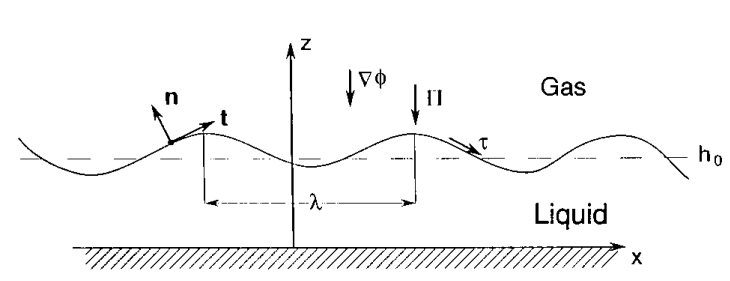
\includegraphics[width=0.76\linewidth]{figures/thin_film_sketch}
%	
%	\caption{Геометрия задачи для тонких слоев, иллюстрация из статьи \cite{Oron1997}  } 
%	\label{fig:thin_film_sketch}
%\end{figure*}


%\textcolor{red}{Представленный обзор охватывает ??три?? основных класса физических эффектов, определяющих динамику тонких жидких пленок: гравитационные, термокапиллярные и вибрационные. Каждый из них в отдельности формирует богатую феноменологию — от солитоноподобных волн при стекании пленок до колебательной конвекции Марангони и параметрических резонансов при вибрационном воздействии. Совместное действие термокапиллярных эффектов и вибраций представляет собой менее изученную область, в которой сосредоточены ключевые вопросы настоящей работы.}

\subsubsection{Гравитационные эффекты: стекание тонких пленок}
%\addcontentsline{toc}{subsection}{Гравитационные эффекты: стекание тонких пленок}

Систематическое изучение поведения тонких пленок началось с экспериментов Тауэра (1883–1884 гг.) по измерению трения и давления в подшипниках скольжения и работы Рейнольдса (1886 год)  \cite{Reynolds1886}, получившего эволюционное уравнение для тонкой пленки в приближении смазки. 

Пионерские работы Капицы \cite{Kapitsa1948a, Kapitsa1948b, Kapitsa1949} по стекающим пленкам заложили основу и наметили круг ключевых вопросов, развитых в последующих исследованиях. Устойчивость невозмущенного слоя с полупараболическим профилем продольной скорости (основное состояние плоской пленки по Нуссельту) была исследована в \cite{Yih1955, Benjamin1957, Yih1963}. Выяснилось, что основное состояние неустойчиво к длинноволновым возмущениям. Бенни расширил \cite{Benney1966} этот анализ, вывел нелинейное динамическое уравнение эволюции межфазной поверхности, в которое входили инерционные слагаемые, гидростатическое давление, капиллярные и вязкие силы. Существенный недостаток построенной модели состоял в том, что уже при умеренных числах Рейнольдса результаты линейного анализа устойчивости уравнения Бенни заметно расходились с результатами, полученными из уравнения Орра--Зоммерфельда.

Уравнение Бенни может быть сведено к уравнению Курамото--Сивашинского \cite{Nepomniashchii1974, Kuramoto1975, Kuramoto1976, Sivashinsky1977} -- хорошо изученному уравнению, допускающему лишь ограниченные решения: стационарные, периодические, квазипериодические или хаотические \cite{Hyman1986, Kevrekidis1990}.

Слабонелинейный анализ \cite{Lin1969, Gjevik1970} показал, что характер перехода к нелинейному режиму определяется волновым числом возмущения: при волновых числах выше порогового двумерные волны насыщаются, ниже порогового — неограниченно нарастают за конечное время. Для вертикальной пластины равновесные двумерные волны неустойчивы как к трехмерным возмущениям, порождающим периодические поперечные структуры \cite{Joo1992a}, так и к субгармоническим двумерным возмущениям \cite{Joo1992b}.

Как уже было сказано, принципиальное ограничение уравнения Бенни состоит в том, что его применимость ограничена малыми числами Рейнольдса. Для описания течений при умеренных и больших числах Рейнольдса Шкадов \cite{Shkadov1967, Shkadov1968} предложил модель, в которой инерция учитывается в ведущем порядке, а уравнение эволюции заменяется системой уравнений для толщины пленки и объемного расхода. 

Для описания волновых явлений в тонких жидких пленках при относительно больших числах Рейнольдса, когда длинноволновые модели теряют применимость, широко используется модель мелкой воды, где теория строится на основе осреднения поля скорости по глубине пленки, а также на интегральном законе сохранения массы. Выбор замыкания для профиля скорости определяется режимом течения: для ламинарных течений традиционно используется полупараболический профиль, тогда как для турбулентных -- профиль типа «поршневого течения» (plug flow). В уравнение импульса входит безразмерный параметр, учитывающий донное трение, а для предотвращения образования ударных волн в модель нередко вводится искусственная вязкость -- подход, обоснованный в \cite{Needham1984, Chang2000}.


Рассмотренные выше модели относятся к изотермическому случаю. При наличии нагрева динамика пленки определяется не только инерционными и гравитационными силами, но и температурными эффектами, что требует учета температурного поля при построении модели.

Важную роль в изучении волновых явлений и механизмов неустойчивости в тонких пленках на локально нагретых пластинах сыграли исследования О.А. Кабова и его соавторов, которые начались с работ \cite{Kabov1998, Kabov2001}. В \cite{Kalliadasis2003} была разработана модель специально для описания этих экспериментов, с помощью метода взвешенных невязок. Было показано, что устойчивое состояние пленки обусловлено конкуренцией между гравитационными силами и поверхностными силами, возникающими вследствие локального нагрева. При этом данное состояние неустойчиво к возмущениям в поперечном направлении. Модель давала предсказания критического числа Марангони и длин волн пальцеобразных структур, порядок величины которых совпадал с экспериментальными данными Кабова. Однако детальное количественное сравнение было затруднено, так как в модели задавалось условие постоянной температуры стенки, тогда как в экспериментах поддерживался постоянный тепловой поток.
В дальнейшем эти модели были последовательно уточнены -- добавлены эффекты вязкой диссипации \cite{RuyerQuil2005, Scheid2005}, а также применено более физически обоснованное условие теплового потока на границе жидкость-твердое тело \cite{Trevelyan2007}, что позволило, в частности, обнаружить солитонные волны с «отрицательными горбами».

В настоящий момент очень большое число работ посвящено динамике стекающих тонких пленок. Помимо уже упомянутых работ \cite{Oron1997, Chang2002, Craster2009} их результаты обобщены в ряде монографий и статей \cite{Alekseenko1994, Kalliadasis2012, RuyerQuil2014}.


\subsubsection{Термокапиллярная конвекция }
%\addcontentsline{toc}{subsection}{Термокапиллярная конвекция }

В неизотермических задачах с межфазной границей динамика определяется конкуренцией объемных и поверхностных сил. Капиллярные эффекты обычно слабее объемных (в частности, архимедовых), но существует широкий круг задач, в которых их роль оказывается определяющей: динамика свободной границы в условиях невесомости, течения с фазовыми включениями, а также течения тонких пленок.

Поверхностные силы в таких задачах определяются градиентом коэффициента поверхностного натяжения вдоль границы раздела фаз. В зависимости от природы этого градиента различают термо-, концентрационно- и электрокапиллярную конвекцию. Исторически первые исследования капиллярного переноса были посвящены концентрационному механизму в попытке объяснить эффект <<слез>> вина \cite{Thomson1855}. Систематическое изучение этого явления провел Марангони \cite{Marangoni1865}, и сегодня все виды такого переноса нередко объединяют под названием эффекта Марангони.

При термокапиллярной конвекции градиент коэффициента поверхностного натяжения порождается неоднородностью температуры вдоль свободной поверхности. Подобные условия реализуются, в частности, при нагреве подложки или наличии тепловых потоков на границах области течения. Возникающие при этом касательные напряжения существенно влияют как на стационарное распределение толщины пленки, так и на ее устойчивость к возмущениям и становятся основным механизмом течения в отсутствие наклона подложки.

Отметим важное обстоятельство -- приближение Обербека -- Буссинеска \cite{Oberbeck1879, Boussinesq1903} (называемое в основном приближением Буссинеска), которое очень часто используется в неизотермических постановках в гидродинамических задачах, не является приемлемым для термокапиллярной конвекции в случае свободных деформируемых границ \cite{Nepomniashchii1983, Drasin1981}. Впервые альтернативная приближению Буссинеска модель для описания неизотермических задач в случае пониженной гравитации была предложена Пухначевым в \cite{Pukhnachev1992}. В \cite{Lyubimov1998}  Любимовым и соавторами было предложено обобщение приближения Буссинеска для учета термокапиллярной и термогравитационной конвекции. 

%Исследование термокапиллярного механизма неустойчивости для случая недеформируемой свободной границы было впервые проведено Пирсоном в работе \cite{Pearson1958}.  В ней был аналитически определен порог возникновения монотонной моды неустойчивости, а также было показано, что в тонком слое ($\sim 1 mm$) развитие неустойчивости связано с термокапиллярными, а не термогравитационными эффектами. В работе \cite{Gershuni1972} было показано, что причина возникновения неустойчивости в горизонтальном слое жидкости на твердой подложке со свободной деформируемой границей зивисит от толщины слоя. В слоях толщиной $\sim 1 mm$ и меньше основной вклад вносят капиллярные силы, в толстых слоях, наоборот, этим механизмом можно пренебречь. Механизм развития неустойчивости описан в \cite{Gershuni1972, Davis1987}.

%Задача в которой учитывалась деформация свободной поверхности при нагреве снизу была впервые рассмотрена в \cite{Scriven1964}. Оказалось, что учет деформации поверхности понижает порог коротковолновую моду, а при этом длинноволновые возмущения неустойчивы во всем диапазоне волновых чисел. Колебательная длинноволновая мода неустойчивости при нагреве сверху была впервые обнаружена в работе \cite{Takashima1981}. 

 Первое теоретическое исследование термокапиллярного механизма неустойчивости для недеформируемой границы было выполнено Пирсоном \cite{Pearson1958}, который показал, что в тонких слоях ($ \sim 1 $ мм и менее) неустойчивость определяется именно термокапиллярными, а не термогравитационными эффектами. Более точная оценка, позволяющая определить, при какой толщине слоя термокапиллярная конвекция становится доминирующим механизмом, была получена Бирихом \cite{Birikh1966}. 
 
 Сравнение вкладов этих механизмов можно проводить с помощью безразмерных чисел Марангони и Рэлея:
 
 
 \[
 \mathrm{Ma} = - \frac{d \alpha(T)}{d T}  \frac{A c_0}{\rho \nu^2}, \quad \mathrm{Ra} = \frac{A g \beta  c_0^3}{\nu \chi},
 \]
 где $c_0$ -- толщина невозмущенного слоя жидкости, $T$ -- температура, $A$ -- характерный перепад температуры, $\alpha(T)$ -- коэффициент поверхностного натяжения, $\rho$ -- плотность жидкости, $\beta$ -- коэффициент объемного теплового расширения, $\nu$ -- коэффициент кинематической вязкости, $\chi$ -- коэффициент температуропроводности, $g$ -- ускорение свободного падения. 
 
Число Марангони, характеризующее интенсивность термокапиллярного переноса, содержит толщину слоя как линейный множитель, тогда как число Рэлея, отвечающее за термогравитационный перенос, -- как кубический. Поэтому, например, для воды при характерных толщинах ($\sim 10^{-4} $ м) число Рэлея оказывается мало по сравнению с числом Марангони и термокапиллярный механизм превалирует над термогравитационным. Таким образом, динамика тонких пленок в неизотермических условиях определяется прежде всего термокапиллярной конвекцией. 

Рассмотрим работы, посвященные задачам о термокапиллярной конвекции в тонком слое жидкости на горизонтальной твердой подложке. Предполагается линейная зависимость коэффициента поверхностного натяжения от температуры и отрицательное значение его производной по температуре.
В \cite{Pimputkar1980} рассматривалась двумерная постановка с фиксированной температурой на свободной поверхности. Копбосыновым и Пухначевым  \cite{Kopbosynov1983} получено эволюционное уравнение для динамики межфазной границы в трехмерном случае с граничным условием третьего рода и проведен линейный анализ устойчивости плоской невозмущенной границы.
Задача с учетом деформации свободной поверхности при нагреве снизу была впервые рассмотрена в  \cite{Scriven1964}. Оказалось, что учет деформации понижает порог коротковолновой моды, а длинноволновые возмущения неустойчивы во всем диапазоне волновых чисел. Колебательная длинноволновая мода неустойчивости при нагреве сверху была впервые обнаружена в \cite{Takashima1981}.
Наряду с однослойным подходом, в котором теплообмен через границу раздела учитывается посредством граничного условия, существует двухслойный подход, в котором уравнения теплопереноса решаются как в жидкой, так и в газовой фазе  \cite{VANHOOK1997, Golovin1995, GOLOVIN1997, Samoilova2015}.


При анализе устойчивости термокапиллярной конвекции в случае свободной верхней границы раздела важным является выбор скейлинга для числа Био, капиллярного числа и числа Галилея:
\[
\mathrm{Bi} = q \frac{c_0}{\kappa}, \mathrm{Ca} = \frac{\alpha c_0}{\rho \nu \chi}, \mathrm{Ga} = \frac{g c_0^3}{\nu \chi},
\]
где $q$ -- параметр, характеризующий интенсивность теплопотока со свободной границы жидкости в невесомый газ, $\kappa$ -- коэффициент теплопроводности.

Так, в случае больших чисел Галилея ($Ga \sim 10^2 $) \cite{Andreev2000} деформацию поверхности можно считать несущественной \cite{Nield1964, VANHOOK1997}. В длинноволновом приближении в случае $\mathrm{Bi} \sim O(\varepsilon^4), \mathrm{Ga} \gg 1$, эволюция системы сводится к уравнению для температуры \cite{Knobloch1990}, случай $\mathrm{Bi} \sim O(\varepsilon^4), \mathrm{Ca} \sim O(1)$ рассматривается в \cite{GarciaYbarra1987}, при   $\mathrm{Bi} \sim O(1), \mathrm{Ga} \sim O(1)$ система сводится к одному уравнению для координаты границы раздела (см. \cite{Oron1997, Samoilova2021}). 

Начиная с работы Пирсона \cite{Pearson1958} принято рассматривать два вида твердых подложек: идеально теплопроводящая -- в этом случае температура жидкости фиксирована на подложке и подложка с очень низкой теплопроводностью -- на подложке фиксируется нормальная составляющая теплового потока. Подложку такого типа в литературе называют <<подложкой, изолированной для возмущений>>. Эта конфигурация изучалась в \cite{Shklyaev2010, Shklyaev2012} и предполагалось $\mathrm{Bi} \sim O(\varepsilon^2), \mathrm{Ca} \sim O(\varepsilon^{-2}), \mathrm{Ga} \sim O(1)$. В этих работах найдены нейтральные кривые для монотонной и колебательной неустойчивости и показано, что для тонких слоев жидкости колебательная мода может быть опасна при подогреве снизу. 


В \cite{Samoilova2015} исследована колебательная конвекция Марангони в тонком слое жидкости в рамках двухслойной модели. Показано, что получаемые эволюционные уравнения для координаты межфазной границы и температуры содержат уточнения по сравнению с результатами \cite{Shklyaev2010, Shklyaev2012}, проявляющиеся в нелинейных слагаемых, описывающих теплопотери через границу раздела. Установлено, что результаты линейного анализа устойчивости, полученные в рамках однослойной модели, хорошо согласуются с результатами двухслойного подхода. При этом в двухслойной постановке эмпирический параметр, характеризующий эффективность теплообмена, заменяется на более физически обоснованные характеристики жидкой и газовой фаз. В \cite{Samoilova2014} для линеаризованной исходной системы уравнений без введения скейлинга для безразмерных параметров аналитически было получено выражение для монотонной моды, а также численно был установлен более широкий диапазон значений для колебательной моды. В \cite{Sarma2018} аналитически в рамках линейного анализа были получены нейтральные кривые для монотонной и колебательной моды неустойчивости для длинноволновых и коротковолновых возмущений.  

Отметим также важное обстоятельство: в реальных физических системах довольно сложно получить абсолютно чистую межфазную границу жидкости, свободную от примесей (загрязнений). В случае наличия примесей (сурфактантов) необходимо учитывать еще один механизм, а именно -- концентрационную конвекцию и дополнять математическую постановку уравнением для переноса концентрации, а также учитывать изменение коэффициента поверхностного натяжения вследствие изменения концентрации на границе раздела (см., например, \cite{Mizev2014, Mikishev2015, Mikishev2019}).

К отдельным разделам относятся работы, в которых изучаются формирование паттернов на свободной поверхности жидкости, учет фазовых переходов, когда рассматриваемая конвекция осложнена испарением со свободной границы, неравномерный нагрев подложки или нелинейную зависимость коэффициента поверхностного натяжения от температуры. Некоторые из этих результатов обобщены в ряде монографий, статей и диссертационных работ \cite{Tan1990, Davis1987, Andreev2000, Schatz2001, Zuev2011monogr, Shklyaev2017, Lyulin2017, Nepomnyashchy2023}.  

%................................................................................................................

%\textcolor{blue}{Оценим характерное значение, когда термокапиллярная конвекция превалирует над термогравитационной. }

%................................................................................................................

%\textcolor{blue}{	Также оценим порог, когда пленку можно считать тонкой или ультратонкой.}

%................................................................................................................

%\textcolor{blue}{Экспериментов нет, но прямое численное моделирование должно быть?}

%................................................................................................................

\subsubsection{Тонкие пленки магнитной жидкости}
%\addcontentsline{toc}{subsection}{Тонкие пленки магнитной жидкости }

Магнитные жидкости (МЖ), называемые также ферромагнитными жидкостями или феррожидкостями, представляют собой устойчивые коллоидные суспензии однодоменных ферро- или ферримагнитных наночастиц размером порядка 10 нм, взвешенных в немагнитной жидкости-носителе -- керосине, воде, минеральных или синтетических маслах \cite{Cowley1989, Shliomis1974}. Для предотвращения слипания частиц под действием ван-дер-ваальсовых и магнитодипольных сил притяжения их поверхность покрывают слоем поверхностно-активного вещества, обеспечивающим стерическую стабилизацию коллоида \cite{Blum1989}.

Теоретическую базу механики МЖ (феррогидродинамику) заложили Дж. Ноирингер и Р. Розенцвейг \cite{Neuringer1964}, предложившие замкнутую систему уравнений, объединяющую уравнения Навье--Стокса с дополнительной пондеромоторной силой. Изложение феррогидродинамики и термомеханики МЖ дано в монографиях \cite{Cowley1989, Berkovskiy1989, Bashtovoy1989, Blum1989}. 

Наиболее известным и исследованным явлением на свободной поверхности МЖ является неустойчивость Розенцвейга. Суть явления заключается в следующем. Если горизонтальный слой МЖ со свободной поверхностью поместить в однородное магнитное поле, направленное по нормали к невозмущенной поверхности, то при полях ниже некоторого критического значения поверхность остается плоской, а при достижении критического значения на ней спонтанно возникает статическая периодическая структура пиков. В \cite{Cowley1967} аналитически в линейной постановке было получено критическое волновое число возмущений для невязкого полубесконечного слоя. 

В \cite{Salin1993} был проведен линейный анализ с учетом вязкой диссипации и получено дисперсионное соотношение для возмущений поверхности раздела. В \cite{Abou1997} получено единое дисперсионное соотношение для слоя произвольной толщины и вязкости. Было показано, что оно зависит от толщины слоя, а также были получены критические значения полей и волновых чисел для толстого и тонкого слоев, а также для вязкой и инерционной динамики жидкости. 

В \cite{Zelazo1969} проведен анализ воздействия на границу раздела для произвольно направленного магнитного поля, в частности показана возможность стабилизации границы тангенциально направленным полем. На основе разложения по малому надкритическому параметру в \cite{Gailtis1977} было показано, что вблизи порога устойчивости возникает гексагональная структура пиков, при дальнейшем увеличении поля возникают квадратные ячейки, получена бифуркационная диаграмма возникновения паттернов на поверхности.  

В \cite{Bashtovoi1985} исследовался слой толщиной более 50 мкм в закритической области значений магнитного поля. В \cite{Dikanskii2010} экспериментально исследовалась неустойчивость плоских горизонтальных слоев МЖ толщиной от 5 до 50 мкм в перпендикулярном магнитном поле при закритических значениях величины напряженности магнитного поля, исследована зависимость характера возникающей структуры поверхности слоя от величины внешнего магнитного поля и толщины слоя. В \cite{Zakinyan2013} экспериментально исследована неустойчивость тонкого слоя феррожидкости, расположенного на намагничивающейся подложке. Показано, что использование магнитной подложки снижает порог возникновения неустойчивости и изменяет характеристики возникающих поверхностных структур. В \cite{Zakinyan2017} экспериментально исследована неустойчивость сверхтонких слоев МЖ (до 50 мкм). Показано образование различных поверхностных структур (гребней и гексагональных пиков), изучены условия их формирования, измерены волновые характеристики и время развития неустойчивости, а также исследовано разрушение тонких слоев.
 
 В \cite{Korovin2013} исследована модель тонкого слоя МЖ, позволяющая описать начальную стадию развития неустойчивости Розенцвейга. Было определено критическое значение намагниченности, при котором плоская свободная поверхность слоя теряет устойчивость, а также соответствующее пороговое волновое число, характерная длина волны и время роста наиболее неустойчивого возмущения. Кроме того, получено аналитическое выражение для кривой нейтральной устойчивости. 
 
 В \cite{Khokhryakova2021} рассматривалась свободная граница МЖ на жидкой подложке в переменном вертикальном магнитном поле и изучена длина получающихся волновых структур в зависимости от характеристик поля. В \cite{Khokhryakova2024} исследован распад плавающего слоя МЖ на упорядоченную систему капель в постоянном вертикальном поле, определена зависимость критического поля от толщины слоя.

В \cite{ZakinyanAhmed2024} экспериментально изучена неустойчивость границы раздела проводящей МЖ и диэлектрической немагнитной жидкости при одновременном действии постоянных магнитного и электрического полей, перпендикулярных границе, и установлена связь между критическими значениями напряженности поля и электрического напряжения. 


\subsubsection{Вибрационные эффекты в жидких пленках}
%\addcontentsline{toc}{subsection}{Вибрационные эффекты в тонких пленках }

%Физический механизм развития неустойчивости при нагреве? подложки ? следующий. При возникновении деформации свободной границы возникает область локального прогиба и в этом месте межфазная поверхность  оказывается в зоне повышенной температуры относительно невозмущенных соседних участков. При этом, предполагая монотонное  убывание коэффициента поверхностного натяжения как функцию температуры, получаем, что межфазные касательные напряжения, пропорциональные тангенциальному градиенту поверхностного натяжения вдоль границы раздела фаз, обуславливают отток жидкости из зоны прогиба. Вследствие вязкой природы жидкости указанный отток сопровождается вязким увлечением прилегающих слоев, что приводит к увеличению локального прогиба и истончению пленки. Ни гидростатические силы давления, ни капиллярные силы не способны подавить данную неустойчивость \cite{Oron1997}. Одним из механизмов стабилизации является вибрационное воздействие. 



Как правило, вибрационные задачи гидродинамики рассматриваются в малоамплитудном высокочастотном приближении. То есть рассматриваются задачи, в которых вибрационное время (период вибраций) много меньше остальных гидродинамических времен (вязкого и теплопроводного), что позволяет получить замкнутую систему уравнений для осредненных и пульсационных полей. Подобный прием разделения физических полей был применен Капицей в известной задаче о маятнике с вибрирующей точкой подвеса \cite{Kapitsa1951a, Kapitsa1951b}.

Широко известно, что вибрационное воздействие способно подавлять разного рода неустойчивости. В экспериментальных работах Вольфа  \cite{Wolf1969, Wolf1970} было показано подавление неустойчивости Рэлея–Тейлора в горизонтальной двухслойной системе под действием вертикальных высокочастотных вибраций. Теоретический линейный анализ данной задачи с использованием метода осреднения выполнен Черепановым  \cite{Cherepanov1984}, подробное изложение содержится в монографии  \cite{Lyubimov2003}. Длинноволновая неустойчивость в аналогичной системе исследовалась в \cite{Lapuerta2001}.

В \cite{Ptrlis2000} экспериментально было показано, что вертикальные вибрации сосуда с МЖ подавляют неустойчивость Розенцвейга, а измеренный сдвиг критического значения поля количественно согласуется с аналитической моделью на основе теории функций Матьё. 

%Обобщение этих результатов на неизотермический случай было выполнено Тиле, Вегой и Кноблохом \cite{20}, где дополнительно учитывался эффект Марангони и подробно исследовалось соответствующее амплитудное уравнение.

Другой известной особенностью влияния вибраций является параметрическое возбуждение, возникающее, когда частота внешнего воздействия сопоставима с одной из собственных частот системы (например, с частотой капиллярно-гравитационных волн). Такие волны наблюдались Фарадеем \cite{Faraday1831} на поверхности горизонтального слоя жидкости при вертикальных колебаниях. Линейный и нелинейный анализ параметрической неустойчивости проводился, в частности, в \cite{Benjamin1954, Lyubimov2003, Mancebo2002}, среди которых наиболее детальным исследованием линейных аспектов неустойчивости Фарадея является работа \cite{Mancebo2002}.

В \cite{Mller1998}  классическая теория Фарадея была обобщена на случай наличия постоянного нормального магнитного поля для случая с вязкой диссипацией для слоев конечного размера. Было показано, что параметрическое воздействие приводит к увеличению времени развития неустойчивости Розенцвейга. В \cite{Mahr1998a, Mahr1998b} была экспериментально исследована как <<магнитная>> фарадеевская неустойчивость, возбуждаемая переменным во времени магнитным полем, так и нелинейная динамика одиночного пика Розенцвейга при модуляции поля и было установлено, что в зависимости от частоты и амплитуды модуляции она может как стабилизировать, так и дестабилизировать пик. 

В \cite{Mekhonoshin2002} был выполнен линейный анализ устойчивости слоя МЖ конечной глубины при одновременном действии вертикальных вибраций и горизонтального магнитного поля. Была обнаружена возможность управления ориентацией и симметрией возникающих волновых структур. 

В \cite{Wang2025} экспериментально построена подробная фазовая диаграмма состояний свободной поверхности МЖ в переменном вертикальном магнитном поле в широком диапазоне частот и амплитуд. Выделены диапазоны существования режима фарадеевских волн и режима пиков Розенцвейга, получены степенные зависимости пороговых значений обоих режимов от частоты и предложена единая волновая модель, объясняющая отбор волнового числа и устойчивость квадратной симметрии по сравнению с гексагональной.

%\textcolor{red}{У нас то все-таки не ультратонкие пленки?} 

В задачах с ультратонкими пленками использование высокочастотного приближения физически неоправданно, так как для  характерной невозмущенной толщины пленки $\sim 100-1000 \textup{~\AA} $ для соответствия оценке $t_{\omega} = 2 \pi / \omega \ll t_{\nu} = c_0^2/\nu$, необходимы частоты $\omega$ порядка 100 МГц и выше, что труднодостижимо в эксперименте. В \cite{Shklyaev2008} предложен альтернативный подход, позволяющий обойти указанное ограничение. Вместо предельного случая высоких частот рассматривается режим умеренных частот при большой амплитуде вибрации, сравнимой или превышающей среднюю толщину пленки. На основе приближения смазки и метода осреднения движение жидкости представляется в виде суммы быстроосциллирующей (пульсационной) и медленно меняющейся (осредненной) компонент. Вводится, помимо разделения физических полей, иерархия времен -- появляется <<быстрое время>> $\sim O(1)$ и <<медленное время>> $\sim O(\varepsilon^2)$. В результате выводится нелинейное амплитудное уравнение для эволюции толщины пленки. Показано, что в определенной области параметров отсутствуют как параметрическая, так и сдвиговая неустойчивости пульсационного течения. Численные и аналитические исследования демонстрируют, что вибрационное воздействие в этом режиме способно стабилизировать систему, подавляя развитие неустойчивости.

Дальнейшее развитие данного подхода представлено в \cite{Shklyaev2009}, где исследуется влияние продольных и наклонных вибраций. С использованием метода многих масштабов исходная полная система уравнений разделяется на осциллирующую и осредненную составляющие, при этом частота вибрации предполагается достаточно высокой, чтобы инерционные эффекты играли существенную роль в быстрой компоненте движения. Выводится амплитудное уравнение, учитывающее вклад гравитации, поверхностного натяжения, потенциала сил Ван-дер-Ваальса и вклад вибрационного воздействия. Показано, что продольные вибрации приводят к дестабилизации плоской поверхности раздела. Установлено, что при таком вибрационном воздействии существуют устойчивые решения, при которых межфазная граница находится в возмущенном (не плоском) состоянии. В случае наклонных вибраций возможны как стабилизация, так и дестабилизация системы в зависимости от параметров системы. Тем самым демонстрируется, что механическое воздействие в виде вибрации может служить эффективным инструментом управления устойчивостью тонких пленок.

Для вибрационных задач с тонкими пленками в рамках длинноволнового 
приближения можно выделить три основных подхода в зависимости от 
безразмерной частоты вибраций $\Omega$. В первом случае $\Omega \sim 
\varepsilon$ мала и линейные и нелинейные члены уравнения эволюции 
толщины пленки $c_0$ зависят от времени~\cite{Halpern2001, Oron2002}. 
Во втором случае $\Omega \sim O(1)$, то есть частота конечна. Тогда 
удается получить единое автономное нелинейное уравнение для осредненной 
динамики $c_0$ на медленном времени~\cite{Shklyaev2008, Shklyaev2009}. 
В третьем случае используется приближение смазки (число Рейнольдса $\mathrm{Re} \ll 1$) 
и в уравнениях удерживаются инерционные слагаемые, что приводит к системе из нескольких 
уравнений эволюции~--- для толщины пленки и объемного 
расхода~\cite{Bestehorn2013, Rojas2010, Rojas2011}.

Отдельного внимания заслуживает природа неустойчивости Фарадея в тонких пленках. В случае продольно неограниченной пленки критическая 
длина волны $L_F$ не превышает толщины пленки $c_0$, то есть 
неустойчивость Фарадея является коротковолновой~\cite{Shklyaev2015}. 
Это отличает ее от длинноволновой термокапиллярной 
неустойчивости Марангони и накладывает ограничения на 
применимость длинноволновых моделей. В частности, одновременное 
использование длинноволнового приближения и приближения смазки 
для описания коротковолновой фарадеевской моды $L_F \lesssim c_0$  \cite{Rojas2010, Rojas2011} внутренне противоречиво \cite{Shklyaev2015}. 

%Именно это противоречие возникает в 
%работах~\cite{Rojas2010, Rojas2011}.

%	где $\mathrm{Re} = \omega c_0^2/\nu \sim 1$: введение характерной вертикальной скорости $V_0$ приводит к избыточному 
%	числу параметров, а для восстановления согласованности авторы вынуждены 
%	дополнительно использовать соотношение $\mathrm{Re}\Omega = \omega 
%	c_0^2/\nu$, что делает безразмерную частоту $\Omega \sim 
%	1/\mathrm{Re}$ большой при $\omega \sim \nu/c_0^2$~\cite{Shklyaev2015}. 
%	Тем самым формальное применение длинноволнового приближения оказывается 
%	направленным на описание заведомо коротковолновой фарадеевской 
%	неустойчивости, что, по-видимому, не вполне корректно.

Особый класс задач составляют системы, в которых одновременно действуют термокапиллярные эффекты и внешнее вибрационное воздействие. Для неизотермических вибрационных задач замкнутая система уравнений для осредненных и пульсационных полей впервые получена Зеньковской  \cite{Zenkovskaya1966}. Следует отметить, что для задач со свободной деформируемой поверхностью приближение Буссинеска при вибрационном воздействии некорректно. Обобщение этого приближения предложено Любимовым  \cite{Lyubimov1994, Lyubimov1995}. Обстоятельное изложение основ термовибрационной конвекции для задач с твердыми границами содержится в монографии  \cite{Gershuni1998}.

Если вибрационное время сопоставимо или меньше остальных гидродинамических времен (случай конечных частот), разделение на осредненные и пульсационные поля становится невозможным. Анализ термовибрационной конвекции при конечных частотах показывает, что независимость амплитуды и частоты вибраций может приводить к параметрическому резонансу  \cite{Wadih1988}. В этих условиях необходимо использование моделей без осреднения, учитывающих эффекты параметрического возбуждения  \cite{Gershuni1996}.

В \cite{Lappa2016} численно исследовано использование синусоидальной модуляции гравитации для управления формированием конвективных структур в жидкости с малым числом Прандтля в замкнутой полости. В \cite{Smorodin2016} проведено аналитическое исследование устойчивости конвекции в горизонтальном слое жидкости для твердых горизонтальных стенок при горизонтальных вибрациях произвольной частоты. Асимптотически определены критические значения параметров в случае малых амплитуд и низких частот внешних вибраций.

Влияние периодической модуляции межфазного теплообмена на нелинейные волны Марангони в горизонтальной двухслойной пленке исследовано в~\cite{Simanovskii2020, Nepomnyashchy2020}: численный анализ длинноволновых амплитудных уравнений выявил режимы чередующихся валиков и осциллирующих квадратов, а также явление синхронизации. При этом собственная частота марангониевских колебаний становится соизмеримой с частотой внешнего воздействия, и течение нередко изменяет пространственную структуру.

Влияние параметрического возбуждения на неустойчивость Марангони в тонком ограниченном горизонтальном слое жидкости, нагреваемом снизу при отсутствии силы тяжести, рассмотрено в~\cite{Ignatius2024}. На основе линейного анализа устойчивости и нелинейных расчетов в рамках редуцированной модели показано, что длинноволновая мода, ответственная за образование сухих пятен, может быть подавлена параметрическим воздействием, тогда как коротковолновая мода остается практически нечувствительной. При низких частотах существует конечный диапазон амплитуд, в котором достигается полная линейная стабилизация пленки; при превышении критической частоты такая стабилизация невозможна. Тем не менее нелинейный механизм насыщения, связанный с вихревыми структурами под волнами Фарадея, существенно уменьшает деформации поверхности и препятствует образованию сухих пятен.


Взаимодействие параметрического резонанса и термокапиллярной неустойчивости в слое жидкости со свободной поверхностью, подверженной вертикальным вибрациям и заданному вертикальному градиенту температуры, исследовалось также в \cite{Birikh2001, Mikishev2025}. В~\cite{Birikh2001} методом многих масштабов в приближении малой вязкости показано, что при совместном действии вибраций и температурного градиента при достаточно большой амплитуде вибраций возбуждаются волны Фарадея. Их частота вдвое меньше частоты вынуждающего воздействия, причем их амплитуда зависит от числа Марангони, а критическая амплитуда возбуждения с ростом числа Марангони сначала убывает относительно порога чисто фарадеевской неустойчивости, проходит через минимум и затем монотонно возрастает с увеличением температурного градиента. При этом порог зоны устойчивости оказывается не зависящей от частоты и амплитуды вибраций. В \cite{Mikishev2025} изучалась устойчивость волн Фарадея на свободной поверхности жидкости с поверхностно-активным веществом при вертикальных вибрациях и вертикальном градиенте температуры в полубесконечном слое. Показано, что без вибрации возникает неустойчивость Левченко-Чернякова, а при включении вибрации появляется параметрический резонанс, интервал которого расширяется с ростом амплитуды вибрации и при определенных условиях переходит в случай, изученный ранее в \cite{Birikh2001} .

В \cite{Ignatius2025} задача рассмотрена для вязкоупругой жидкости. Показано, что упругость качественно меняет картину устойчивости и вместо единственной верхней границы по частоте, характерной для ньютоновского случая, на карте нейтральной устойчивости в плоскости амплитуда--частота возникает устойчивая зона, ограниченная как снизу, так и сверху по частоте. Вне этой зоны пленка одновременно подвержена неустойчивости Марангони и неустойчивости Фарадея. Кроме того, вязкоупругость снижает пороговые амплитуды на границе нейтральной устойчивости для обоих типов неустойчивостей. Авторы связывают это с эффектом памяти, вносимым упругостью жидкости.


 В \cite{Permyakova2023} рассмотрено параметрическое возбуждение свободной тепловой конвекции в горизонтальном слое под действием стохастического воздействия. 

%Неустойчивость Релея–Тейлора расширяет диапазон линейно неустойчивых мод. Стабилизация такого типа неустойчивости за счет термокапиллярных эффектов рассматривалась в работах \cite{Oron1992, Deissler1992}. Было показано, что при нагреве свободной поверхности или охлаждении твердой подложки возможно насыщение неустойчивости Релея–Тейлора и формирование стационарных капель.

В \cite{Shklyaev2015} исследована термокапиллярная конвекция в тонкой пленке жидкости на вертикально колеблющейся подогреваемой пластине в широком диапазоне частот -- от сверхнизких до высоких. В рамках длинноволнового приближения получены амплитудные уравнения и выполнен линейный и слабонелинейный анализ устойчивости. Показано, что при высоких частотах колебаний эффективное поверхностное натяжение возрастает, однако разрыв пленки сохраняется; при сверхнизких частотах вибрация действует как модуляция силы тяжести и приводит к быстрому подкритическому росту деформаций поверхности. В промежуточном диапазоне частот вибрация либо практически не влияет на конвекцию, либо возбуждает неустойчивость с меньшей длиной волны. Установлено также, что граница вибрационной неустойчивости Марангони располагается ниже границы неустойчивости Фарадея, тогда как высокочастотные колебания подавляют конвекцию Марангони и способствуют развитию неустойчивости Фарадея.


\newpage


\subsection{Метод решеточных уравнений Больцмана}
%\addcontentsline{toc}{subsection}{Метод решеточных уравнений Больцмана}

Особенность численного моделирования задач со свободной границей в вибрационных полях заключается в необходимости одновременного разрешения нескольких физически различных, но взаимосвязанных явлений: (i) эволюции подвижной, деформируемой границы раздела фаз с учетом поверхностного натяжения; (ii) взаимодействия компонентов с существенно различающимися физическими свойствами (плотность, вязкость); (iii) нестационарного внешнего силового воздействия, задаваемого вибрацией, которое модулирует эффективное поле массовых сил и может приводить к движению межфазной границы.

Описание задач, связанных со свободной границей раздела между двумя несмешивающимися компонентами среды при отсутствии фазовых переходов, может быть построено несколькими способами. В рамках механики сплошной среды, если не рассматривать спектральные методы, эти подходы можно разделить на два класса: метод резкой границы раздела (Sharp Interface Method) и метод диффузной границы раздела (Diffuse Interface Method) \cite{Anderson1998, Udaykumar2001, Demont2023}.
В методе резкой границы раздела определяющие уравнения решаются только в одной из сред, при этом дополнительное уравнение для определения положения границы раздела не вводится. Предполагается, что граница раздела имеет нулевую толщину, а физические величины испытывают на ней разрывы. К числу широко известных численных методов, реализующих данный подход, относятся метод Level-Set, метод Volume-of-Fluid (VOF) и комбинированный метод Coupled Level-Set and VOF (CLSVOF). Два последних метода характеризуются большой точностью выполнения закона сохранения массы \cite{Hirt1981, Sethian2003, Wang2009, Ningegowda2014}.
В методе диффузной границы раздела граница обладает конечной толщиной, а физические величины изменяются через нее непрерывно, без разрывов. Такой подход требует введения дополнительного эволюционного уравнения, описывающего динамику границы раздела. В качестве таких уравнений могут использоваться уравнения Кана–Хилларда или Аллена–Кана. В частности, они являются незаменимыми при решении задач, в которых граница раздела претерпевает топологические изменения, например при слиянии или распаде капель \cite{Cahn1958, Cahn1959, Allen1976, Anderson1998, Lamorgese2011}.
Сравнительной оценке указанных подходов посвящен ряд работ (см., например \cite{Shaikh2018, Liu2019, Zhang2025}).

С середины второй половины прошлого века начал набирать популярность метод решеточных уравнений Больцмана (Lattice Boltzmann Method, LBM), исторически связанный с более ранними моделями решеточных газовых автоматов (Lattice Gas Cellular Automata) \cite{WolfGladrow2005}. Метод в его современной форме, свободной от статистического шума, присущего решеточным газовым автоматам, был впервые предложен в \cite{McNamaraZanetti1988}. %, а затем существенно развит благодаря введению линейного (BGK) оператора столкновения \cite{Qian1992}%.
Особенно интенсивно его применение в моделировании различных систем выросло в последние десятилетия \cite{Li2020, ChenDoolen1998}. По данным сайта ScienceDirect.com число публикаций, содержащих аббревиатуру LBM в названии, за 25 лет увеличилось примерно на порядок.

Вычислительный алгоритм метода в самом простом изотермическом случае может быть выведен из кинетического уравнения Больцмана \cite{BOLTZMANN2003, Lifshitz1981}, в котором, как известно, вводится статистическое представление ансамбля частиц.
Эволюция системы описывается функцией распределения, зависящей от времени, радиус-вектора и скорости элемента фазового объема. 
%В правую часть эволюционного уравнения входит слагаемое, отвечающее за действие внешних сил на элемент фазового объема, а также интеграл столкновений, отвечающий за релаксацию системы к локальному статистическому равновесию.

Описание системы строится на мезоскопическом масштабе, занимающем промежуточное положение между характерными масштабами молекулярной динамики и сплошной среды. Макроскопические параметры среды -- плотность, импульс и энергия -- выражаются через нулевой, первый и второй моменты функции распределения соответственно (см., например, \cite{Samarskii2001}).

Для практического использования кинетического уравнения Больцмана применяется линеаризованное приближение интеграла столкновений в форме Бхатнагара--Гросса--Крука (Bhatnagar--Gross--Krook, BGK) \cite{Lifshitz1981, Bhatnagar1954}, в рамках которого вводится равновесная функция распределения (распределение Максвелла) и единый параметр времени релаксации системы. При условии близости системы к состоянию локального термодинамического равновесия и малости числа Кнудсена (характеризующего степень разреженности потока частиц) из линеаризованного кинетического уравнения могут быть выведены классические уравнения гидродинамики -- уравнение неразрывности, уравнение Навье–Стокса и закон сохранения энергии \cite{Qian1992, Succi2018, Redeman2014, Samarskii2001, Lifshitz1981}.

%Первым шагом построения численного алгоритма является дискретизация исходного континуального уравнения Больцмана. Эта процедура нетривиальна, поскольку исходное уравнение сформулировано для фазового пространства повышенной размерности (пространственные координаты, скорость, время), и в него, помимо прочего, входит производная функции распределения по мезоскопической скорости.

Дискретизированное уравнение Больцмана может быть получено из континуального несколькими путями \cite{Succi2018}. Наиболее строгий и формальный из них основан на разложении функции распределения в пространстве скоростей по полиномам Эрмита с последующим применением квадратуры Гаусса–Эрмита, обобщенной на произвольную размерность пространства \cite{Succi2018, Redeman2014, Krger2017}.

Поскольку для восстановления макроскопических характеристик течения  (плотности, импульса и энергии) достаточно первых моментов функции распределения, в разложении по полиномам Эрмита можно ограничиться лишь несколькими первыми членами ряда, не учитывая члены более высокого порядка. Такой подход позволяет получить дискретизированную равновесную функцию распределения, зависящую от плотности и скорости потока, а также от весовых коэффициентов и дискретных направлений скорости, отвечающих узлам квадратуры Гаусса–Эрмита и от скорости звука в модели (см., например, \cite{Krger2017}).

Дискретное эволюционное уравнение (решеточное уравнение) записывается для набора функций распределения, соответствующих конечному числу разрешенных направлений скорости. При численном моделировании это уравнение на каждой временной итерации распадается на два последовательных шага \cite{Krger2017, Succi2018}: шаг столкновения (collision), на котором в каждом узле решетки вычисляется эволюция функции распределения и шаг переноса (streaming), на котором результаты столкновения без изменений переносятся вдоль соответствующих дискретных направлений скорости в соседние по направлению узлы. Такое разделение на локальную (collision) и нелокальную (streaming) операции обеспечивает высокую эффективность распараллеливания алгоритма, поскольку большая часть вычислений (столкновение) выполняется независимо в каждом узле. Макроскопические параметры среды восстанавливаются суммированием функции распределения или равновесной функции распределения по всем дискретным направлениям скорости после столкновения.

Выбор скоростной модели (числа узлов квадратуры) определяет значения весовых коэффициентов, набор разрешенных дискретных скоростей и величину скорости звука в модели \cite{Viggen2014, WolfGladrow2005, Latt2007}.

%Вторым шагом построения численного алгоритма является выбор скоростной модели, то есть числа узлов квадратуры. Этот выбор определяет значения весовых коэффициентов, набор разрешенных дискретных скоростей и величину скорости звука в модели \cite{Viggen2014, WolfGladrow2005, Latt2007}.

%В настоящей работе используется скоростная модель D2Q9, соответствующая двумерному физическому пространству с девятью разрешенными направлениями дискретной скорости. Конкретные числовые значения весовых коэффициентов и набора скоростей приведены, например, в \cite{Krger2017}.

С помощью разложения Чепмена–Энскога \cite{Chapman1991} дискретная модель, при условии малости чисел Маха и Кнудсена, может быть сведена к уравнениям неразрывности и Навье–Стокса. При этом устанавливается прямая связь между параметром времени релаксации и коэффициентом кинематической вязкости среды \cite{Krger2017, Succi2018}.

Помимо простейшего оператора столкновения BGK с одним временем релаксации (Single Relaxation Time, SRT), широко используются более сложные операторы столкновения, обеспечивающие повышенную точность и численную устойчивость \cite{Krger2017, Succi2018}. В частности, в методе с множественными временами релаксации (Multiple-Relaxation-Time, MRT), предложенном в \cite{dHumires2002}, столкновение выполняется не в пространстве самих функций распределения, а в пространстве их моментов. Функции распределения линейно преобразуются в набор моментов, включающий плотность, компоненты импульса, тензор напряжений и моменты более высокого порядка. Каждый момент релаксирует со своей скоростью, определяемой соответствующим временем релаксации. После решения эволюционного уравнения выполняется обратное преобразование в пространство функций распределения. Такой подход позволяет независимо управлять релаксацией моментов функции распределения, что существенно повышает устойчивость схемы при малых значениях вязкости и позволяет уменьшить эффекты, связанные с фиксированной в BGK-модели связью времени релаксации и коэффициента кинематической вязкости \cite{dHumires2002, Krger2017, Succi2018}.
Промежуточным по сложности между BGK и MRT моделями является метод с двумя временами релаксации (Two-Relaxation-Time, TRT) \cite{Ginzburg2003, Ginzburg2005, Ginzburg2008}, в котором функция распределения разделяется на симметричную и антисимметричную части, релаксирующие с двумя различными временами. При этом надлежащий выбор соотношения между ними
%(так называемого «магического параметра») 
позволяет устранить некоторые эффекты дискретизационных погрешностей, в частности зависимость эффективного положения твердой стенки от вязкости при использовании простых схем отражения на границе \cite{Ginzburg2008, Krger2017}.

Реализация граничных условий в LBM также имеет ряд особенностей по сравнению с традиционными методами вычислительной гидродинамики, поскольку граничные условия формулируются не для макроскопических полей скорости и давления, а непосредственно для функций распределения на границе расчетной области. Наиболее простой и широко используемой схемой является схема отражения (bounce-back), в которой компоненты функции распределения, направленные внутрь твердой границы, разворачиваются в противоположном направлении. Эта схема физически соответствует условию прилипания и, в зависимости от точного положения условной стенки, относительно узлов решетки, обеспечивает первый или второй порядок точности по пространству \cite{Krger2017, Succi2018}.

Учет внешних массовых сил (в частности, силы тяжести, а также вибрационной силы) осуществляется путем введения дополнительного источникового слагаемого в правую часть дискретного эволюционного уравнения, которое модифицирует как этап столкновения, так и восстанавливаемый из функций распределения макроскопический импульс среды \cite{Krger2017, Succi2018}. 

%Корректный учет данного слагаемого необходим для устранения дискретизационных погрешностей второго порядка по параметру решетки, которые в противном случае могут вносить нефизичный вклад в эффективную вязкость и, как следствие, искажать структуру течения, индуцируемого внешним силовым полем \cite{Krger2017}.

Необходимо отметить, что все параметры модели -- время, длина, скорость, плотность и производные от них величины -- задаются в безразмерных решеточных единицах, связанных с физическими единицами через параметры решетки. Корректный переход между решеточной и физической системами единиц является отдельной существенной частью постановки численного эксперимента \cite{Krger2017, Succi2018}.

Метод решеточных уравнений Больцмана обладает рядом ограничений, которые необходимо учитывать. Классические алгоритмы, как правило, применимы лишь к слабосжимаемым течениям с малыми числами Маха. Кроме того, LBM требует большего объема памяти по сравнению с традиционными методами вычислительной гидродинамики, поскольку в каждом узле расчетной сетки необходимо хранить полный набор дискретных функций распределения. Обеспечение устойчивости вычислений при больших значениях безразмерных параметров, больших отношениях плотностей и кинематических вязкостей фаз требует тщательного подбора параметров релаксации. Иногда может потребоваться применение более сложных операторов столкновения, о которых говорилось выше, вместо простейшей BGK-модели.

\subsubsection{LBM для задач со свободной границей раздела} 

В рамках LBM существует несколько подходов к описанию задач со свободными деформируемыми границами раздела \cite{Krger2017, Succi2018, Huang2015, Sukop2006, Inamuro2021, Preprint2025, Wang2019, Chen2014, Li2016, Chen2026, Cao2020}. Эти подходы можно разделить на четыре класса: метод цветового градиента (color-gradient method), в котором каждой фазе сопоставляется своя <<цветная>> функция распределения, а граница между фазами задается через градиент разности цветов \cite{Gunstensen1991, Zahid2025}; псевдопотенциальная модель, в которой вводится феноменологическая сила межчастичного взаимодействия \cite{Shan1993}; метод свободной энергии, в котором равновесная функция распределения и тензор давления строятся так, чтобы согласоваться с заданным термодинамическим функционалом свободной энергии \cite{Swift1995} и фазово-полевой метод, в котором динамика границы раздела описывается дополнительным уравнением эволюции параметра порядка, согласованным с уравнениями гидродинамики \cite{He1999-1, He1999-2}. В некоторых классификациях два последних объединяются в одну категорию \cite{Krger2017, Inamuro2021, Li2016}. Все перечисленные подходы реализуют метод диффузной границы раздела. По-видимому, реализация метода резкой границы раздела в рамках LBM также возможна через корректное задание граничных условий при использовании метода погруженной границы (Immersed Boundary Method) \cite{Inamuro2021, Cao2020}.

Фазово-полевой и псевдопотенциальный подходы широко применяются при практическом моделировании многофазных течений. Общим недостатком обоих методов является возникновение паразитных скоростей (spurious currents) в области границы раздела \cite{Krger2017, Chen2014, Li2016}. Несмотря на то, что метод псевдопотенциала успешно применяется, его математическая постановка основана на феноменологической силе взаимодействия и не выводится непосредственно из термодинамически согласованного функционала свободной энергии. Это затрудняет строгую аналитическую интерпретацию модели и ее непосредственную связь с макроскопическими уравнениями механики сплошной среды. 
%Поэтому в настоящей работе используется фазово-полевой метод как более термодинамически обоснованная альтернатива.

В случае фазово-полевой постановки конечная толщина диффузной границы раздела может приводить к сглаживанию мелкомасштабных межфазных структур, если ее величина не является достаточно малой по сравнению с характерными масштабами течения. При выборе параметров численного моделирования указанные ограничения необходимо принимать во внимание.

Макроскопическое описание в методе фазового поля основывается на уравнении Кана--Хилларда (КХ) \cite{Cahn1958, Cahn1959} или уравнении Аллена--Кана (АК) \cite{Allen1976}. Важно отметить, что исходное уравнение АК не является консервативным относительно массы; поэтому в рамках LBM используется консервативная формулировка данного уравнения \cite{Chiu2011, Geier2015}.

В изотермической постановке макроскопическое описание включает уравнения Навье--Стокса, уравнение неразрывности (в сжимаемой или несжимаемой форме), а также уравнение для параметра порядка (АК или КХ), дополненные соответствующими начальными и граничными условиями. В LBM данный подход использует два набора функций распределения: один для эволюции импульса, а другой --- для эволюции параметра порядка или поля давления.

Существенной и фундаментальной проблемой данного класса алгоритмов является то, что они зачастую не обеспечивают сохранение массы и не всегда корректно восстанавливают уравнение для параметра порядка. Кроме того, в LBM для восстановления уравнения параметра порядка используется локальное уравнение эволюции функции распределения. В макроскопическом пределе такой подход не приводит к уравнению КХ, поскольку последнее является уравнением четвертого порядка и требует использования нелокальных конечно-разностных схем для вычисления пространственных производных \cite{Wang2019, Li2016}.

Кратко рассмотрим развитие фазово-полевых моделей в рамках LBM. Первая модель была предложена в 1999 году Хе, Ченом и Чжаном (модель HCZ) \cite{He1999-1, He1999-2, Zhang2000}. Модель HCZ позволяла восстановить макроскопическую систему, содержащую уравнение КХ, при этом уравнение неразрывности формулировалось для сжимаемых течений. К существенным недостаткам данной модели относятся относительная сложность реализации и ограничение на применение к задачам с небольшими отношениями плотностей двух компонентов. Данный алгоритм был использован для моделирования <<замороженной>> волны \cite{Volodin2020, Volodin2021}.

В \cite{Inamuro2004} была представлена модель, позволившая проводить моделирование задач с отношением плотностей вплоть до $\rho_{r}=\rho_l / \rho_g=1000$, где индекс $l$ обозначает тяжелую фазу, а $g$ --- легкую. В соответствующей макроскопической модели используется приближение несжимаемой жидкости и уравнение КХ. Последующие усовершенствования алгоритма были предложены авторами в \cite{Inamuro2016, Inamuro2018, Inamuro2021}. В \cite{Lee2005} был предложен трехэтапный алгоритм стабилизации для двухфазных течений, позволяющий проводить моделирование при больших отношениях плотностей. Однако, как отмечается в ряде исследований (например, в \cite{Hu2018}), данный подход существенно снижает простоту программной реализации, которая обычно рассматривается как одно из преимуществ LBM.

В ряде исследований для отслеживания границы раздела фаз использовалась консервативная форма уравнения АК \cite{Geier2015, Fakhari2016, Fakhari2017, Ren2016, Wang2016, Chai2018, Liu2014, Hong2023, Liang2018}. Сравнительный анализ уравнений АК и КХ в контексте LBM представлен в \cite{Wang2016}, где показано, что подходы, основанные на консервативном уравнении АК, обладают более высокой численной устойчивостью. Кроме того, в обзоре \cite{Wang2019} отмечается, что LBM-схемы, использующие данный подход, в целом характеризуются повышенной численной устойчивостью.

При выборе схемы, использующей консервативное уравнение АК для описания границы раздела фаз, остается принципиальным вопрос о выборе его локальной \cite{Geier2015, Fakhari2016, Ren2016}, нелокальной \cite{Chai2018, Liu2014, Hong2023} или гибридной \cite{Hu2019} формы. В \cite{Chai2018} показано, что как локальная, так и нелокальная формы уравнения АК обеспечивают сохранение массы как всей системы, так и каждой отдельной фазы. При этом локальная форма более точно воспроизводит профиль границы раздела, тогда как нелокальная форма обеспечивает большую численную устойчивость. Гибридный подход \cite{Hu2019} позволяет уменьшить влияние дискретизации на точность решения.

Таким образом, учитывая большое разнообразие LBM-подходов для моделирования многокомпонентных сред и течений со свободно деформируемой поверхностью, выбор конкретной схемы является нетривиальной задачей. Тем не менее, несмотря на большое число исследований, посвященных методу решеточных уравнений Больцмана для моделирования многофазных течений, ограниченное число работ рассматривает вибрационное воздействие как фактор, определяющий динамику системы. Так, в \cite{Chang2010} исследуется фазовое разделение в бинарной жидкости под действием вибрации. В \cite{DOrazio2020} развиваются граничные условия применительно к тестовой задаче об осциллирующих стенках путем модификации гидродинамической и тепловой функций распределения. В \cite{Volodin2020, Volodin2021} моделируются поверхностные волны и квазистационарный рельеф границы раздела, возникающие под вибрационным воздействием.

%В настоящей работе предпочтение отдается схеме, основанной на консервативной нелокальной форме уравнения Аллена--Кана.

%Несмотря на значительное количество исследований, посвященных методу решеточных уравнений Больцмана для моделирования многофазных течений в последние годы (см., например, \cite{Ibrahim2025, Kang2025, Thirumalaisamy2025, Otomo2025}), 

%лишь ограниченное число работ рассматривает вибрационное воздействие как фактор, определяющий динамику системы. Так, в работе \cite{Chang2010} методом LBM исследуется фазовое разделение в бинарной жидкости под действием вибрации. В \cite{DOrazio2020} развиваются граничные условия LBM применительно к тестовой задаче об осциллирующих стенках путем модификации гидродинамической и тепловой функций распределения. В работах \cite{Volodin2020, Volodin2021} методом решеточных уравнений Больцмана моделируются поверхностные волны и квазистационарный рельеф границы раздела, возникающие под вибрационным воздействием.

Отметим также, что, несмотря на огромную популярность метода решеточных уравнений Больцмана, подтверждаемую в том числе существованием нескольких мощных открытых программных платформ, реализующих LBM -- например, Palabos \cite{Latt2021}, OpenLB \cite{Krause2021}, waLBerla \cite{Bauer2021}, Swalbe \cite{Zitz2019, Zitz2022}, в отечественной научной среде метод пока не получил столь широкого распространения. Например, число диссертационных работ, посвященных непосредственно методу решеточных уравнений Больцмана и его приложениям, защищенных в России, остается весьма ограниченным. Среди них можно отметить кандидатскую диссертацию Д.А. Медведева, посвященную моделированию гидродинамических и электрогидродинамических течений решеточными методами \cite{Medvedev2002}, докторскую диссертацию А.Л. Куперштоха, в которой метод решеточных уравнений Больцмана применяется для моделирования электрического пробоя жидких диэлектриков и предшествующих ему гидродинамических течений \cite{Kuperstokh2006}, кандидатскую диссертацию Б.В. Сидоренко, посвященную разработке и реализации параллельных алгоритмов решеточного метода Больцмана для моделирования гидродинамических процессов \cite{Sidorenko2012}, сравнительно недавнюю кандидатскую диссертацию Н.С. Гибанова, посвященную нестационарным режимам сопряженного конвективного теплопереноса в замкнутых областях, выполненную с использованием LBM \cite{Gibanov2021}, а также докторскую диссертацию Г.В. Кривовичева, в которой решеточные уравнения Больцмана рассматриваются в общем контексте гиперболических моделей процессов переноса и применяются, в частности, к задачам гемодинамики \cite{Krivovichev2022}.

%Такое положение дел свидетельствует об актуальности дальнейшего развития и адаптации метода решеточных уравнений Больцмана применительно к задачам российской научной школы, в частности к задачам динамики свободных границ в вибрационных полях, рассматриваемым в настоящей работе.

Таким образом, сохраняется актуальность дальнейшего развития метода решеточных уравнений Больцмана и расширения круга задач, для которых он применяется, включая задачи динамики свободных границ в вибрационных полях.




\mychapter{2}{Термокапиллярная конвекция тонкого слоя жидкости под воздействием вертикальных вибраций}{chap:thermo}



Данная глава посвящена исследованию динамики тонкого слоя жидкости с приложенным вертикальным градиентом температуры под воздействием вертикальных вибраций. Метод решения включает в себя разделение полной системы уравнений на пульсационные и осредненные поля.

Получена динамическая система осредненных уравнений, решена линейная задача устойчивости тонкой пленки. Осредненная система проинтегрирована численно методом Radau IIA, построены карты устойчивости течений при разных значениях чисел Марангони и Галилея.  

Результаты опубликованы в работах \cite{Volodin2025, Volodin2026Averaged}.

\subsection{Система уравнений термокапиллярной конвекции под действием вибраций}

Рассматривается динамика тонкой, бесконечной в продольном направлении, вязкой, несжимаемой жидкой пленки, расположенной на плоской горизонтальной твердой подложке, $c_0$ -- толщина пленки в невозмущенном состоянии (см. рис. \ref{fig:problem_statement_thermal}). Верхняя поверхность пленки свободна и деформируема, над ней находится невесомый газ. Поперек слоя задан постоянный вертикальный отрицательный температурный градиент. Подложка совершает вертикальные гармонические колебания с частотой $\omega$ и амплитудой $b$.

\begin{figure}
	\centering
	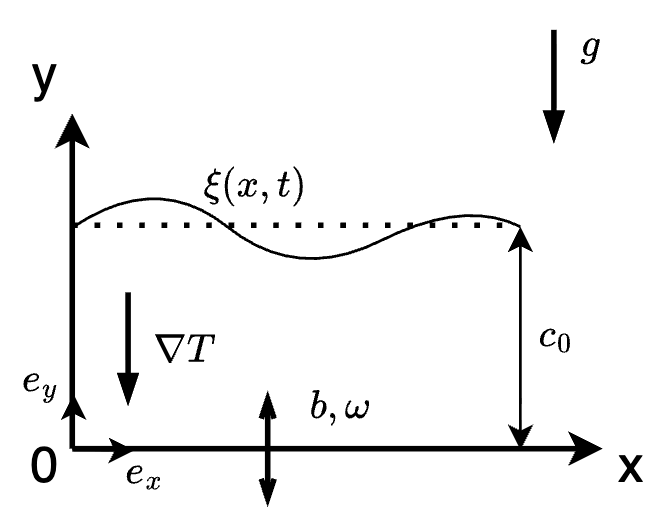
\includegraphics[width=0.45\linewidth]{figures/chap2/problem_statement2.png}
	\caption{Геометрия задачи}
	\label{fig:problem_statement_thermal}
\end{figure}

Необходимо учитывать изменение коэффициента поверхностного натяжения вдоль границы раздела, обусловленное неизотермической постановкой. Задача описывается следующей системой уравнений:
\begin{equation}
	\nabla \cdot \mathbf{v} = 0,
\end{equation}
\begin{equation}
	\rho \left( \frac{\partial \mathbf{v}}{\partial t} + (\mathbf{v} \cdot \nabla)\mathbf{v} \right) = -\nabla p + \eta \Delta \mathbf{v} + \mathbf{f},
\end{equation}
\begin{equation}
	\frac{\partial T}{\partial t} + (\mathbf{v} \cdot \nabla)T = \chi \Delta T,
\end{equation}
где $\mathbf{v} = (u,v)$ -- скорость жидкости, $T$ -- температура жидкости, $p$ -- поле давления, $\rho$ -- плотность жидкости, $\eta=\rho \nu$ -- коэффициент динамической вязкости жидкости, $\nu$ -- коэффициент кинематической вязкости жидкости,  $\chi$ -- коэффициент температуропроводности, $\mathbf{f}$ -- внешнее силовое поле, $\nabla$ -- векторный дифференциальный оператор первого порядка, $\Delta$ -- скалярный дифференциальный оператор второго порядка.

Когда вибрационная сила направлена вдоль силы тяжести, удобно перейти в неинерциальную систему отсчета, связанную с подложкой \cite{Lyubimov2003, Shklyaev2008, Shklyaev2015, Mancebo2002}. В этом случае внешняя сила $\mathbf{f}$ будет иметь вид: 
\begin{equation*}
	\mathbf{f} = - \rho g \mathbf{e}_y + \rho b \omega^2 \cos(\omega t) \mathbf{e}_y.
\end{equation*}

%Запишем граничные условия после перехода в неинерциальную систему. 
На подложке выполняется условие прилипания и поставлен постоянный тепловой поток через границу:
\begin{equation}
	u = v = 0,
\end{equation}
\begin{equation}\label{eq:low_thermal_diffusivity_bc_thermal}
	\frac{\partial T}{\partial y} = -A_0,
\end{equation}
где $A_0$ определяет интенсивность теплового потока.

На свободной поверхности $y = \xi(x, t)$ должны выполняться следующие условия: кинематическое граничное условие для скорости, непрерывность теплового потока на межфазной границе и условие баланса нормальных и тангенциальных компонент тензора напряжений $\sigma_{ik}$, с учетом зависимости коэффициента поверхностного натяжения $\alpha(T)$ от температуры. Кинематическое условие и условие непрерывности теплового потока записываются в виде:
\begin{equation}\label{eq:surface_velocity_bc_thermal}
	\frac{\partial \xi}{\partial t} + u \frac{\partial \xi}{\partial x} = v,
\end{equation}
\begin{equation}\label{eq:one_layer_bc_thermal}
	\mathbf{n} \cdot (\nabla T) = -\frac{q}{\kappa} T,
\end{equation}
где $\mathbf{n}$ -- вектор, направленный по нормали к поверхности   $y = \xi(x, t)$, $q$ -- коэффициент теплоотдачи между свободной поверхностью и невесомым газом, $\kappa$ -- коэффициент теплопроводности подложки.

Граничные условия для тензора напряжений в индексной форме записи имеют вид \cite{Birikh2003}:
\begin{equation*}
	\left( \sigma^{ (1)}_{ik} - \sigma^{ (2)}_{ik} \right) n_k = \alpha \frac{\partial n_l}{\partial x_l} n_i - \left( \frac{\partial}{\partial x_i} - n_i n_l \frac{\partial}{\partial x_l} \right)\alpha,
\end{equation*}
где цифры $(1)$ и $(2)$ обозначают значение величины в жидкости и газе, соответственно. По повторяющимся индексам предполагается суммирование.

Тензор напряжений записывается в виде:
\begin{equation*}
	\sigma_{ik} = -p \delta_{ik} + \eta \left( \frac{\partial v_i}{\partial x_k} + \frac{\partial v_k}{\partial x_i} \right),
\end{equation*}
где $\delta_{ik}$ -- дельта-символ Кронекера.

%Как видно из \eqref{eq:one_layer_bc_thermal} используется однослойная модель с пассивной газовой фазой. \textcolor{red}{Теплопроводность подложки считается малой, то есть ее коэффициент теплопроводности много меньше, чем коэффициент теплопроводности воды. Как это связано с \eqref{eq:low_thermal_diffusivity_bc_thermal}?}

Из баланса тангенциальных и нормальных компонент тензора напряжений получим:
\begin{equation}\label{eq:viscous_normal_bc_thermal}
	\left( \sigma^{ (1)}_{ik} - \sigma^{ (2)}_{ik} \right) n_i n_k = \alpha \frac{\partial n_l}{\partial x_l} n_i n_i,
\end{equation}
\begin{equation}\label{eq:viscous_tangential_bc_thermal}
	\left( \sigma^{ (1)}_{ik} - \sigma^{ (2)}_{ik} \right) n_k \tau_i = -\tau_i \frac{\partial \alpha}{\partial x_i},
\end{equation}
где $\mathbf{\tau}$ -- вектор, тангенциальный к поверхности раздела. Векторы $\mathbf{n}$ и  $\mathbf{\tau}$ находятся из условий:

\begin{equation*}
	\quad \mathbf{n} \cdot \boldsymbol{\tau} = 0, \quad 	\mathbf{n} = \frac{\nabla  F}{|{\nabla  F|} },
\end{equation*}
где $F = y - \xi(x, t)$.

Выбрав в качестве характерных масштабов длину $ c_0 $, время $ c_0^2/\nu $, скорость $\nu/ c_0$, давление $\rho (\nu/c_0)^2$ и  температуру $c_0  |{\frac {\partial T}{\partial y}|  }$, получаем следующую безразмерную систему уравнений:
\begin{equation} \label{eq:dmnsless_div_thermal}
	\nabla \cdot \mathbf{v} = 0,
\end{equation}
\begin{equation}
\frac{\partial \mathbf{v}}{\partial t} + (\mathbf{v} \cdot \nabla)\mathbf{v} = -\nabla p +\Delta \mathbf{v} + (- \mathrm{G} + \mathrm{B^*} \Omega^2 \cos(\Omega t) )\mathbf{e_y},
\end{equation}
\begin{equation}
	\frac{\partial T}{\partial t} + (\mathbf{v} \cdot \nabla)T = \mathrm{Pr}^{-1} \Delta T.
\end{equation}
На подложке $y=0$:
\begin{equation}
	u = v = 0,
\end{equation}
\begin{equation}
	\frac{\partial T}{\partial y} = -1
\end{equation}
и на свободной границе $y=\xi(x, t)$:
\begin{equation}\label{eq:surface_velocity_bc2_thermal}
	\frac{\partial \xi}{\partial t} + u \frac{\partial \xi}{\partial x} = v,
\end{equation}
\begin{equation}
	\nabla_nT=-\mathrm{Bi^*} T,
\end{equation}
\begin{equation}  \label{eq:dmnsless_bc_thermal}
	-\mathrm{Ma} \nabla_{\tau} T + (p + \phi - \mathrm{Ca^*} K) \mathbf{n} = \mathbf{n} \mathbf{\sigma^{(1)}},
\end{equation}
где $K=\nabla \cdot \mathbf{n}$ -- кривизна границы, $\nabla_{n}$ и $\nabla_{\tau}$ -- нормальный и тангенциальный дифференциальные операторы, соответственно, $\phi(\xi)$ -- притягивающий потенциал сил Ван-дер-Ваальса, определенный в виде:
\begin{equation*}
	\phi(\xi) = - \frac{A'}{6 \pi \xi^3},
\end{equation*}
где $A'>0$ - константа Гамакера \cite{Dzyaloshinskii1961}. 

%Как будет видно из дальнейших оценок значений управляющих параметров, в рассматриваемой задаче потенциалом сил Ван-дер-Ваальса можно пренебречь. Однако на данном этапе мы не будем исключать этот параметр из рассмотрения, что позволит сохранить общность постановки и проверить корректность предельных переходов путем сопоставления с ранее опубликованными результатами.

Управляющие параметры задачи следующие:
\begin{equation*}
\begin{aligned}
	\mathrm{Ma} &= -\frac{d \alpha}{dT}  \abs{\frac{\partial T}{\partial y} } \frac{c_0^2}{\rho \nu^2}, \quad
	\mathrm{G} = \frac{g c_0^3}{\nu^2}, \quad
	\mathrm{Bi^*} = \frac{q c_0}{\kappa}, \\
	\mathrm{Pr} &= \frac{\nu}{\chi}, \quad
	\mathrm{Ca^*} = \frac{\alpha c_0}{\rho \nu^2}, \quad
	A = \frac{A'}{6 \pi \rho \nu^2 c_0}, \\
	\varphi &= -\frac{A}{\xi^3}, \quad
	\mathrm{B}^{*} = \frac{b}{c_0}, \quad
	\Omega = \omega \frac{c_0^2}{\nu},
\end{aligned}
\end{equation*}
где $\mathrm{Ma}$ -- число Марангони, $\mathrm{G}$ -- число Галилея, $\mathrm{Bi^*}$ -- число Био, $\mathrm{Pr}$ -- число Прандтля, $\mathrm{Ca^*}$ -- капиллярное число, ${A}$ -- безразмерная константа Гамакера, $\mathrm{B^*}$ -- безразмерная амплитуда, $\mathrm{\Omega}$ -- безразмерная частота.


\subsubsection*{Оценки управляющих параметров}\label{sec:governing_params_estimation_thermal}

Проведем оценку значений безразмерных параметров для воды при нормальных (комнатных) условиях:
\[
\rho = 10^3~\text{кг/м}^3,\qquad
\nu = 10^{-6}~\text{м}^2/\text{с},\qquad
\chi = 1.43 \cdot 10^{-7}~\text{м}^2/\text{с},
\]
\[
\alpha = 72.75 \cdot 10^{-3}~\text{Н/м}, \qquad
\frac{d\alpha}{dT} = -1.56 \cdot 10^{-4}~\text{Н/(м·К)}, \qquad
q = 10~\text{Вт}/(\text{м}^2 \cdot \text{К}),
\]
\[
A' = 6\pi \cdot 10^{-21}~\text{Дж}. 
\]
Поскольку коэффициент теплопроводности твердой подложки значительно меньше коэффициента теплопроводности жидкости, будем считать: $\kappa = 0.1~\text{Вт}/(\text{м}\cdot\text{К}).$

Рассмотрим слой жидкости толщиной $c_0 = 10^{-4}~\text{м},$ при перепаде температуры через слой в 1~\text{К}. Пусть также $ b = 10^{-3}~\text{м},\omega = 10^3~\text{рад/с}.$
Тогда значения безразмерных параметров принимают вид
\begin{equation*}
	\mathrm{Ca^*} \approx 7.2 \cdot 10^3,\qquad
	\mathrm{G} \approx 10,\qquad
	\Pr \approx 7,\qquad
	\phi \approx 10^{-8},
\end{equation*}
\begin{equation*}
	\mathrm{Ma} \approx 15,\qquad
	\mathrm{Bi^*} \approx 10^{-2},\qquad
	\mathrm{B^{*}}\approx 10,\qquad
	\Omega \approx 10.
\end{equation*}

Из полученных оценок следует, что для жидких слоев толщиной порядка $10^{-4}$ м при наличии температурного градиента, вклад сил Ван-дер-Ваальса оказывается пренебрежимо малым. Кроме того, число Био является малым параметром, тогда как капиллярный параметр имеет большое значение, остальные безразмерные параметры имеют один и тот же порядок величины. Поэтому далее рассматривается асимптотическое приближение, в котором:
\begin{equation}\label{eq:scaled_Ca_Bi}
	\mathrm{Ca^*}=\varepsilon^{-2}\mathrm{Ca},\qquad
	\mathrm{Bi^*}=\varepsilon^{2}\beta. 
\end{equation}
Потенциал взаимодействия свободной поверхности с твердой подложкой удержим в уравнениях для сопоставления с результатами, полученными в других работах. 

\subsection{Метод решения}


Как уже было сказано, наличие двух характерных пространственных масштабов диктует необходимость введения перемасштабированных пространственных переменных:
\begin{equation} \label{eq:stretched_x_y_vars_thermal}
	X = \varepsilon x, \quad Y = y,
\end{equation}
что приводит к перемасштабированию производных:
\begin{equation}
	\frac{\partial}{\partial x} = \varepsilon \frac{\partial}{\partial X}, \quad
	\frac{\partial}{\partial y} = \frac{\partial}{\partial Y}.
	\label{eq:scaled_derivatives_thermal}
\end{equation}

Компоненты единичных нормального и касательного векторов с точностью до первого порядка по малому параметру принимают вид:
\[
\mathbf{n} =
\left(
-\varepsilon \frac{\partial \xi}{\partial X}, 1
\right),
\qquad
\boldsymbol{\tau} =
\left(
1, \varepsilon \frac{\partial \xi}{\partial X}
\right).
\]

Предполагается, что продольная скорость пропорциональна градиенту давления, то есть:
\[
u = \mathcal{O}(\varepsilon),
\]
что приводит к соответствующему масштабированию продольной компоненты скорости. Из уравнения неразрывности, в свою очередь, определяется масштаб вертикальной компоненты скорости. Таким образом, компоненты скорости выражаются в виде
\begin{equation} \label{eq:stretched_velocity_eq_thermal}
	u = \varepsilon U, \qquad
	v = \varepsilon^2 V.
\end{equation}

Для приведенных выше оценок: $c_0\sim10^{-4} $ $\text{м}$, $\nu\sim10^{-6}\,\mathrm{\text{м}^2/\text{c}}, t_\nu\sim10^{-2}\,\text{c}$
и предполагая частоты $\omega \approx 10^3 $ рад/с, значение вибрационного периода
$t_\Omega\sim10^{-3}$ с.
То есть $t_\nu\gg t_\Omega$ и, соответственно, рассматривается высокочастотное приближение,
$\Omega\sim O(1)$.
Также предполагается, что амплитуды вибраций велики по сравнению с толщиной слоя:
\begin{equation} 
\mathrm{B^*}=\varepsilon^{-1 }\mathrm{B}.
\end{equation}

Наличие высокочастотных вибраций в задаче позволяет разделить исходную систему уравнений, введя иерархию временных масштабов. Динамика «быстрого» (пульсационного) течения определяется вибрационным слагаемым, а в «медленном» (осредненном) течении проявляются накопленные со временем эффекты. Физическая интерпретация данного подхода наглядно представлена в \cite{Kapitsa1951a, Kapitsa1951b, Gershuni1998}, тогда как его математические основы подробно рассмотрены в \cite{Nayfeh1984}.

Введем иерархию временных масштабов следующим образом:
\begin{equation}
	\tilde{t} = \Omega t, \quad \bar{t} = \varepsilon^2 t.
	\label{eq:timescale_hierarchy_thermal}
\end{equation}
При таком преобразовании производная по времени принимает вид:
\begin{equation}
	\frac{\partial}{\partial t}
	=
	\Omega \frac{\partial}{\partial \tilde{t}}
	+
	\varepsilon^2 \frac{\partial}{\partial \bar{t}}.
	\label{eq:time_derivative_expansion_thermal}
\end{equation}

Следующим шагом является представление исходных физических полей в виде суммы пульсационной и осредненной составляющих. Предполагается, что изменение пульсационной составляющей давления определяется главным образом инерционным членом. В соответствии с этим, поле давления представляется в виде:
\begin{equation}
	p = \bar{p} + \frac{\tilde{p}}{\varepsilon},
	\label{eq:pressure_expansion_thermal}
\end{equation}
где черта сверху обозначает осредненную составляющую поля, а тильда -- его пульсационную составляющую. Условие \eqref{eq:pressure_expansion_thermal} приводит к следующему масштабированию компонент скорости:
\begin{equation}
	U = \bar{u} + \frac{\tilde{u}}{\varepsilon},
	\qquad
	V = \bar{v} + \frac{\tilde{v}}{\varepsilon}.
	\label{eq:velocity_scaling_thermal}
\end{equation}

Из анализа уравнения \eqref{eq:surface_velocity_bc_thermal} следует, что координата поверхности должна быть представлена в виде:
\begin{equation}
	\xi = \bar{\xi} + \varepsilon \tilde{\xi},
	\label{eq:interface_expansion_thermal}
\end{equation}
а поле температуры -- в виде:
\begin{equation}
	T = \bar{T} + \varepsilon \tilde{T}.
	\label{eq:T_puls_averaged_expansion_thermal}
\end{equation}

Отметим также, что граничные условия на свободной поверхности
должны быть «снесены» на среднее положение поверхности ($y = \bar{\xi}$).
Для произвольного поля $\mathcal{S}$ получим при этом следующее разложение \cite{Shklyaev2008}:
\begin{equation}\label{eq:bc_Taylor_thermal}
	\mathcal{S}(Y = \bar{\xi} + \varepsilon \tilde{\xi})
	\approx
	\mathcal{S}(\bar{\xi})
	+
	\varepsilon \tilde{\xi}
	\frac{\partial \mathcal{S}(\bar{\xi})}{\partial Y}
	+
	\frac{1}{2}(\varepsilon \tilde{\xi})^2
	\frac{\partial^2 \mathcal{S}(\bar{\xi})}{\partial Y^2}
	+\ldots
\end{equation}


Подставляя разложения \eqref{eq:scaled_Ca_Bi}--\eqref{eq:bc_Taylor_thermal} в безразмерную систему уравнений (\ref{eq:dmnsless_div_thermal})--(\ref{eq:dmnsless_bc_thermal}), получаем две связанные системы уравнений. Одна описывает пульсационное течение на быстром временном масштабе, другая -- осредненное течение на медленном временном масштабе. Осредненная система включает вклад пульсационных компонент. 

\subsection{Пульсационное течение}

	Система уравнений, определяющая пульсационное течение, имеет вид:
\begin{equation}
	\frac{\partial \tilde{u}}{\partial X} + \frac{\partial \tilde{v}}{\partial Y} = 0,
\end{equation}
\begin{equation}
	\Omega \frac{\partial \tilde{u}}{\partial \tilde{t}} = -\frac{\partial \tilde{p}}{\partial X} + \frac{\partial^2 \tilde{u}}{\partial Y^2},
\end{equation}
\begin{equation}
	\frac{\partial \tilde{p}}{\partial Y} =\mathrm{B} \Omega^2 \cos(\tilde{t}),
\end{equation}
\begin{equation}
	\Omega \frac{\partial \tilde{T}}{\partial \tilde{t}} + \tilde{u} \frac{\partial \bar{T}}{\partial X} + \tilde{v} \frac{\partial \bar{T}}{\partial Y} = \frac{1}{\mathrm{Pr}} \frac{\partial^2 \tilde{T}}{\partial Y^2}.
\end{equation}
Граничные условия на подложке \( Y = 0 \) записываются следующим образом:
\begin{equation}
	\tilde{u} =	\tilde{v} = 0,
\end{equation}
\begin{equation}
	\frac{\partial \tilde{T}}{\partial Y} = -1.
\end{equation}
На свободной границе \( Y = \bar{\xi}(X, t) \), граничные условия принимают вид:
\begin{equation}
	\Omega \frac{\partial \tilde{\xi}}{\partial \tilde{t}} + \tilde{u} \frac{\partial \bar{\xi}}{\partial X} = \tilde{v},
\end{equation}
\begin{equation}
	\frac{\partial \tilde{u}}{\partial Y} = 0,
\end{equation}
\begin{equation}
	\tilde{p} = 0,
\end{equation}
\begin{equation}
	\tilde{\xi} \frac{\partial^2 \bar{T}}{\partial Y^2} + \frac{\partial \tilde{T}}{\partial Y} = -\mathrm{\beta} \left( \tilde{\xi} \frac{\partial \bar{T}}{\partial Y} + \tilde{T} \right).
\end{equation}

%?Как будет ясно в дальнейшем? Так как нас интересует вклад пульсационных компонент в осредненное течение, то достаточно решить амплитудную задачу для полей скорости и давления $\tilde{u}, \tilde{v}, \tilde{p}$, полагая

Данная система описывает линейные вынужденные колебания и ее решение ищется в виде:
\begin{align*}
	\tilde{u} &= \Re \left\{ \tilde{A}(X,Y) e^{i \tilde{t}} \right\}, \\
	\tilde{v} &= \Re \left\{ \tilde{B}(X,Y) e^{i \tilde{t}} \right\}, \\
	\tilde{p} &= \Re \left\{ \tilde{C}(X,Y) e^{i \tilde{t}} \right\}, \\
	\tilde{\xi} &=\Re \left\{ \tilde{D}(X) e^{i \tilde{t}} \right\},
\end{align*}
где \( \Re\{\cdot\} \) означает действительную часть выражения, а \( i \) -- мнимая единица. Пульсационная составляющая температурного поля $\tilde{T}$ не входит в осредненные уравнения (см. следующий раздел) и поэтому ее определение не требуется. 

Решение в терминах гиперболических функций имеет вид:

\begin{equation}
	\tilde{A} = i \mathrm{B} \Omega \frac{\partial \bar{\xi}}{\partial X} \left (\frac{\cosh(\theta(Y-\bar{\xi}))}{\cosh(\theta \bar{\xi})} - 1 \right),
\end{equation}

\begin{equation}
	\begin{split}
		\tilde{B} = - i \mathrm{B} \Omega \Biggl(
		\frac{\partial^2 {\bar{\xi}}}{\partial X^2}
		\left(
		\frac{\sinh(\theta(Y-\bar{\xi}))+\sinh(\theta\bar{\xi})}
		{\theta \cosh(\theta \bar{\xi})}
		- Y
		\right)
		\\
		- \left(\frac{\partial \bar{\xi}}{\partial X} \right)^2 \frac{\cosh(\theta Y) - 1}{\cosh^2(\theta \bar{\xi})}  
		\Biggr),
	\end{split}
\end{equation}

\begin{equation}
	\tilde{C} =\mathrm{B} \Omega^2 \left(Y-\bar{\xi}\right),
\end{equation}
\begin{equation}
	\tilde{D} = \frac{i}{\Omega}  \left( \tilde{A} \frac{\partial \bar{\xi}}{\partial X} - \tilde{B} \right),
\end{equation}
где $\theta^2 = -i \Omega$.

\subsection{Осредненное течение}

Система уравнений, определяющая осредненное течение, имеет вид:

\begin{equation}\label{eq:avrg_div_thermal}
	\frac{\partial \bar{u}}{\partial X} + \frac{\partial \bar{v}}{\partial Y} = 0,
\end{equation}
\begin{equation}
	\left\langle \tilde{u} \frac{\partial \tilde{u}}{\partial X} + \tilde{v} \frac{\partial \tilde{u}}{\partial Y} \right\rangle = -\frac{\partial \bar{p}}{\partial X} + \frac{\partial^2 \bar{u}}{\partial Y^2},
\end{equation}
\begin{equation}
	\frac{\partial \bar{p}}{\partial Y} = -\mathrm{G},
\end{equation}
\begin{equation}
	\frac{\partial^2 \bar{T}}{\partial Y^2} = 0,
\end{equation}
где треугольные скобки \(\langle \cdot \rangle\) обозначают процедуру осреднения по пульсационному времени.

Граничные условия на подложке \( Y = 0 \) записываются в виде:
\begin{equation}
	\bar{u} = \bar{v} = 0,
\end{equation}
\begin{equation}
	\frac{\partial \bar{T}}{\partial Y} = -1,
\end{equation}
а на свободной границе \( Y = \bar{\xi}(X, t) \):
\begin{equation}
	\frac{\partial \bar{\xi}}{\partial \bar{t}}
	+ \frac{\partial \bar{\xi}}{\partial X} \left( \bar{u} + \left\langle \tilde{\xi} \frac{\partial \tilde{u}}{\partial Y}  \right\rangle \right)
	+ \left\langle \tilde{u} \frac{\partial \tilde{\xi}}{\partial X} \right\rangle
	= \bar{v} + \left\langle \tilde{\xi} \frac{\partial \tilde{v}}{\partial Y} \right\rangle,
\end{equation}
\begin{equation}
	\frac{\partial \bar{u}}{\partial Y}
	+ \left\langle \tilde{\xi} \frac{\partial^2 \tilde{u}}{\partial Y^2} \right\rangle
	= \mathrm{Ma} \left( \frac{\partial \bar{T}}{\partial X}
	+ \frac{\partial \bar{T}}{\partial Y} \frac{\partial \bar{\xi}}{\partial X} \right),
\end{equation}
\begin{equation}
	\bar{p} + \left\langle \tilde{\xi} \frac{\partial \tilde{p}}{\partial Y} \right\rangle
	+ \mathrm{Ca} \frac{\partial^2 \bar{\xi}}{\partial X^2} = 0,
\end{equation}
\begin{equation}\label{eq:avrg_temp_bc_thermal}
	\frac{\partial \bar{T}}{\partial Y} =- \beta \bar{T}.
\end{equation}

Как видно из анализа получившейся системы, пульсационные компоненты полей входят как квадратичные слагаемые.

\subsection{Осредненные уравнения динамики межфазной границы и температуры}

Система уравнений (\ref{eq:avrg_div_thermal})-(\ref{eq:avrg_temp_bc_thermal}) может быть сведена к системе двух уравнений на межфазной границе. Одно уравнение, при такой редукции, описывает эволюцию положения поверхности раздела, другое уравнение -- эволюцию температуры вдоль поверхности. Такая динамическая система уравнений жесткого типа имеет следующий вид:

%Динамическая система для границы раздела $\bar{\xi}$ и температуры на границе $\bar{T}$ имеет вид, представленный ниже. Здесь и далее мы следуем обозначениям, принятым в работах \cite{Shklyaev2008, Shklyaev2012}. 

\begin{align} \label{eq:avrged_Ma_first_thermal}
	\frac{\partial \bar{\xi}}{\partial \bar{t}}
	&= \frac{\partial}{\partial X} \left(
	\frac{\bar{\xi}^3}{3} \frac{\partial \bar{\Pi}}{\partial X}
	+ \frac{\text{Ma}}{2} \bar{\xi}^2 \frac{\partial f}{\partial X} \right. \notag \\
	&\quad \left. - \frac{(\mathrm{B} \Omega)^2}{2} \left(
	Q_1 \bar{\xi}^2 \left( \frac{\partial \bar{\xi}}{\partial X} \right)^3
	+ Q_2 \bar{\xi}^3 \frac{\partial \bar{\xi}}{\partial X} \frac{\partial^2 \bar{\xi}}{\partial X^2}
	\right)
	\right),
\end{align}
\begin{align} \label{eq:avrged_Ma_second_thermal}
	\frac{\bar{\xi} \, \partial \bar{T}}{\partial \bar{t}}
	&= \frac{1}{\text{Pr}} \frac{\partial}{\partial X} \left( \bar{\xi} \frac{\partial \bar{T}}{\partial X} \right)
	- \frac{1}{2 \, \text{Pr}} \left( \frac{\partial \bar{\xi}}{\partial X} \right)^2
	- \frac{\beta}{\text{Pr}} f  + \left(
	\frac{\bar{\xi}^3}{3} \frac{\partial \bar{\Pi}}{\partial X}
	+ \frac{\text{Ma}}{2} \bar{\xi}^2 \frac{\partial f}{\partial X}
	\right) \frac{\partial f}{\partial X} \notag \\
	&\quad + \frac{\partial}{\partial X} \left(
	\frac{\bar{\xi}^4}{8} \frac{\partial \bar{\Pi}}{\partial X}
	+ \frac{\text{Ma}}{6} \bar{\xi}^3 \frac{\partial f}{\partial X}
	\right),
\end{align}
где $\bar{\Pi} = \mathrm{G} \bar{\xi} - \mathrm{Ca} \frac{\partial^2 \bar{\xi}}{\partial X^2} + \frac{(\mathrm{B} \Omega)^2}{2} \Re\{H\} - \varphi (\bar{\xi}) $, $f=\bar{T} - \bar{\xi}$ -- температурные возмущения на границе и
\begin{align*}
	H = - \frac{\partial}{\partial X} \left[ \bar{\xi} F(\theta \bar{\xi}) \frac{\partial \bar{\xi}}{\partial X} \right], F (\theta \bar{\xi}) = 1 - \frac{\tan(\theta \bar{\xi})}{\theta \bar{\xi}},
\end{align*}
\begin{align*}
	Q_1 = 3 \frac{4 \sinh \gamma \sin \gamma - \gamma (\psi_+ \varphi_+ - \psi_- \varphi_-)}{2 \gamma^2 \psi_+^2},
\end{align*}
\begin{align*}
	Q_2 = -\frac{1}{3} + \frac{11 \varphi_- - 3 \gamma \psi_-}{\gamma^3 \psi_+}, \gamma=\bar{\xi} \sqrt{2 \Omega},
\end{align*}
\begin{align*}
	\psi_+ = \cosh \gamma + \cos \gamma,
	\psi_- = \cosh \gamma - \cos \gamma, \\
	\varphi_+ = \sinh \gamma + \sin \gamma,
	\varphi_- = \sinh \gamma - \sin \gamma.
\end{align*}

Уравнения (\ref{eq:avrged_Ma_first_thermal})-(\ref{eq:avrged_Ma_second_thermal}) описывают осредненную динамику. При отсутствии вибраций (\(\mathrm{B}=0\)) задача сводится к системе, полученной ранее в \cite{Shklyaev2012}, а при отсутствии температурного градиента (\(\beta = \mathrm{Ma} = \bar{T} = 0\)), динамическая система сводится к ранее выведенной в работе \cite{Shklyaev2008}.

\subsection{Анализ устойчивости пленки в линейной постановке}

Рассмотрим динамику свободной границы вблизи порога возникновения неустойчивости. В уравнениях (\ref{eq:avrged_Ma_first_thermal})--(\ref{eq:avrged_Ma_second_thermal}) положим:
\begin{equation*}
\bar{\xi} = 1 + \varepsilon \zeta, \quad \bar{T} = 1 + \varepsilon \Theta.
\end{equation*}
Такая постановка приводит к линеаризованной системе уравнений:
\begin{equation}\label{eq:linear_Ma_first_thermal}
	\frac{\partial \zeta}{\partial \bar{t}} = \frac{1}{3} \frac{\partial^2 \Pi}{\partial X^2} + \frac{\mathrm{Ma}}{2} \frac{\partial^2}{\partial X^2} (\Theta - \zeta),
\end{equation}
\begin{equation}\label{eq:linear_Ma_second_thermal}
	\frac{\partial \Theta}{\partial \bar{t}} = \frac{1}{\mathrm{Pr}} \frac{\partial^2 \Theta}{\partial X^2} - \frac{\beta}{\mathrm{Pr}} (\Theta - \zeta) + \frac{1}{8} \frac{\partial^2 \Pi}{\partial X^2} + \frac{\mathrm{Ma}}{6} \frac{\partial^2}{\partial X^2} (\Theta - \zeta),
\end{equation}
где
\begin{align*}
	\Pi &= \mathrm{G} \zeta - \mathrm{Ca} \frac{\partial^2 \zeta}{\partial X^2} - \frac{(\mathrm{B} \Omega)^2}{2} (1 - m) \frac{\partial^2 \zeta}{\partial X^2} - 3 A \zeta, 
\end{align*}
\begin{equation}	\label{eq:m_vs_omega_thermo}
	m=\frac{\sinh(\gamma_0) + \sin( \gamma_0)}{{\gamma_0}(\cosh(\gamma_0)+\cos(\gamma_0))}, \gamma_0=\sqrt{2\Omega}.
\end{equation}
График функции $m(\Omega)$ приведен на рис. \ref{fig:m_vs_omega_thermo}, из анализа которого видно, что слагаемое $1-m>0$.

\begin{figure}
	\centering
	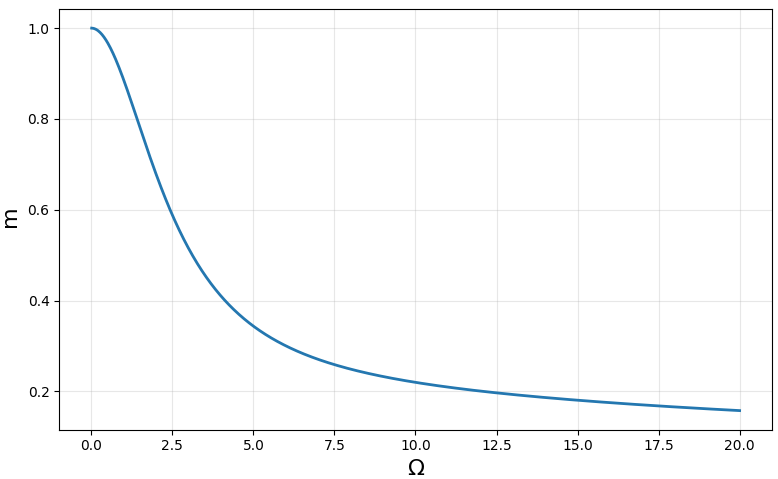
\includegraphics[width=0.705\linewidth]{figures/chap2/m_vs_omega.png}
	\caption{График функции $m(\Omega)$ }
	\label{fig:m_vs_omega_thermo}
\end{figure}


Решение уравнений (\ref{eq:linear_Ma_first_thermal})--(\ref{eq:linear_Ma_second_thermal})  будем искать в виде бегущих волн:
\begin{equation}\label{eq:lambda_view_linear_thermal}
\zeta = \zeta_0 \exp(\lambda \bar{t} + i k X), \quad \Theta = \Theta_0 \exp(\lambda \bar{t} + i k X),
\end{equation}
где $\zeta_0$,  $\Theta_0$ -- амплитуды возмущений, $\lambda$ -- инкремент возмущений, $k=2\pi/L$ -- волновое число возмущений с длиной волны $L$. 

Таким образом, при $\lambda > 0$ возмущения нарастают со временем и это приводит к разрыву пленки, тогда как при $\lambda < 0$ возмущения затухают и межфазная граница стабилизируется.

Подставляя \eqref{eq:lambda_view_linear_thermal} в \eqref{eq:linear_Ma_first_thermal}--\eqref{eq:linear_Ma_second_thermal}, получим уравнение для $\lambda$:

\begin{equation} \label{eq:lambda_Ma_thermal}
	\lambda^2 +\bigg(  \frac{C_2}{48} - C_1 \bigg) \lambda -  \frac{1}{48} (C_1 C_2) + C_3 = 0,
\end{equation}
где:


\begin{align*}
	C_1 =  \bigg(
	& - \frac{1}{3} \mathrm{G} k^2
	- \frac{1}{3} \mathrm{Ca} k^4
	+ \frac{1}{6} \mathrm{B}^2 \Omega^2 k^4 (m-1) + A k^2 + \frac{1}{2} \mathrm{Ma} k^2
	\bigg),
\end{align*}
$$
C_2 = \frac{1}{\mathrm{Pr}} (8 \, \mathrm{Ma} \, \mathrm{Pr} \, k^2 + 48 k^2 + 48 \beta),
$$
$$
C_3 = \frac{\mathrm{Ma} k^2}{96} \bigg(18  (C_1-\frac{1}{2} \mathrm{Ma} k^2) +C_2 - \frac{48 k^2}{Pr}  \bigg) . 
$$


\begin{figure}
	\centering
	\begin{subfigure}[t]{0.48\textwidth}
		\centering
		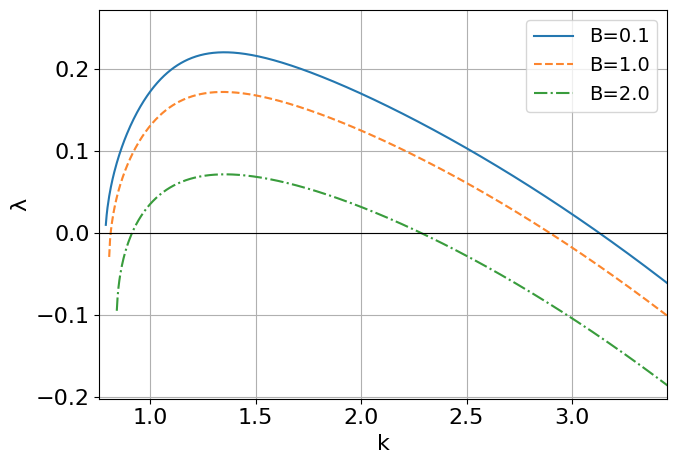
\includegraphics[width=\linewidth]{figures/chap2/B_varies.png}
		\caption{}
		\label{fig:B_varies}
	\end{subfigure}
	\hfill
	\begin{subfigure}[t]{0.48\textwidth}
		\centering
		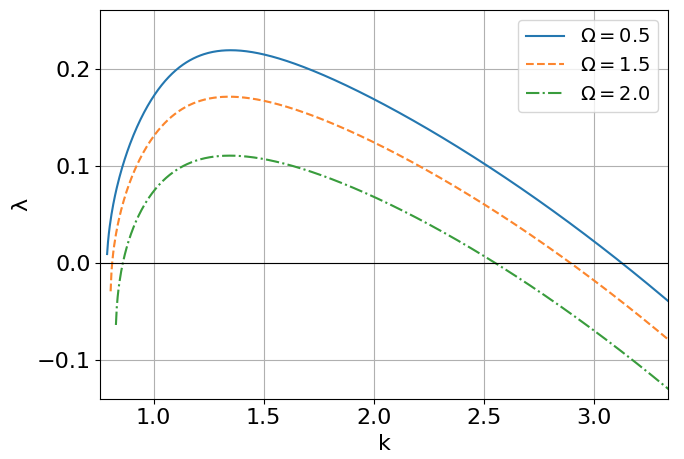
\includegraphics[width=\linewidth]{figures/chap2/Omega_varies.png}
		\caption{}
		\label{fig:Omega_varies}
	\end{subfigure}
	\vspace{0.6cm}
	\begin{subfigure}[t]{0.48\textwidth}
		\centering
		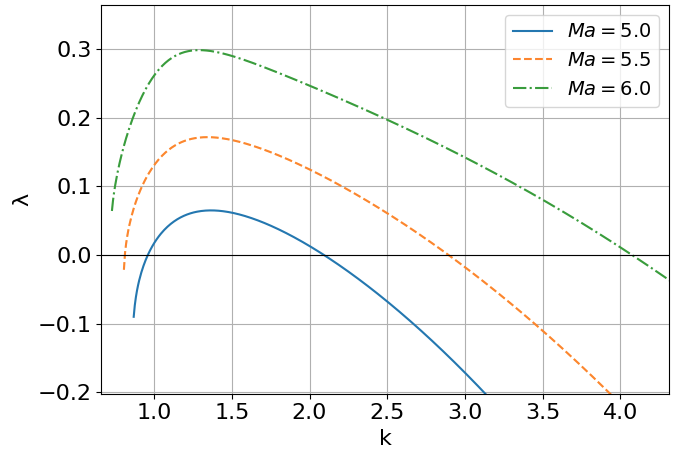
\includegraphics[width=\linewidth]{figures/chap2/Ma_varies.png}
		\caption{}
		\label{fig:Ma_varies_thermal}
	\end{subfigure}
	
	\caption{
		Инкремент возмущений как функция волнового числа для различных управляющих параметров:
		(a) изменение амплитуды внешнего воздействия $\mathrm{B}$
		($\mathrm{Ma}=5.5,\ \Omega=1.5$);
		(б) изменение частоты внешнего воздействия $\Omega$
		($\mathrm{B}=1.0,\ \mathrm{Ma}=5.5$);
		(в) изменение числа Марангони $\mathrm{Ma}$
		($\mathrm{B}=1.0,\ \Omega=1.5$).
		Остальные параметры имеют следующие значения:
		$\mathrm{Ca}=2.5$,
		$\mathrm{G}=3.0$,
		$\mathrm{Pr}=7.0$,
		$\beta=1$.
	}
	\label{fig:linear_stability_thermal}
\end{figure}



В изотермическом случае ($\mathrm{Ma} = \beta= 0$) первый корень уравнения отвечает монотонному затуханию колебаний:
$$
\lambda = -\frac{k^2}{\mathrm{Pr}}.
$$
Второй корень совпадает с полученным ранее в работе \cite{Shklyaev2008}:
\begin{equation*}
	\lambda = \frac{1}{3} k^2 \left( -\mathrm{G} + 3A + k^2 \left[ \frac{(m - 1)}{2}(\mathrm{B} \Omega)^2 - \mathrm{Ca} \right] \right).
\end{equation*}
%Таким образом, в изотермическом случае задача сводится к ранее рассматриваемой в \cite{Shklyaev2008}.

Структура уравнения~(\ref{eq:lambda_Ma_thermal}) показывает, что гравитационные и капиллярные силы стабилизируют свободную поверхность, тогда как нагрев оказывает дестабилизирующее воздействие. В дальнейшем полагается, что притягивающий потенциал Ван-дер-Ваальса в силу своей малости не оказывает влияния на динамику задачи (см. раздел \ref{sec:governing_params_estimation_thermal}).

На рис.~\ref{fig:linear_stability_thermal} представлена скорость роста возмущений как функция волнового числа при
$
\mathrm{Ca}=2.5,
\mathrm{G}=3.0,
\mathrm{Pr}=7.0,
\mathrm{\beta}=1,
$
для различных значений управляющих параметров.
Увеличение амплитуды или частоты вибраций подавляет рост возмущений (см. рис. \ref{fig:linear_stability_thermal}a, \ref{fig:linear_stability_thermal}б) и, следовательно, стабилизирует свободную поверхность, тогда как увеличение числа Марангони оказывает противоположное воздействие, способствуя развитию неустойчивости (рис. \ref{fig:linear_stability_thermal}в).

Для всех выбранных наборов параметров в окрестности $k=0.5$ существует нейтральная область, в которой корни удовлетворяют условию $\lambda^2(k)<0$ и, следовательно, скорость роста $\lambda$ является чисто мнимой.
Остальные ветви дисперсионного соотношения не показаны, поскольку они соответствуют $\Re(\lambda)<0$ и поэтому не влияют на границу устойчивости.


Инкремент возмущений обращается в нуль при следующих значениях волновых чисел:
$\lambda(k_1\approx3.1284)=0$ при $\mathrm{B}=0.1$,
$(k_1\approx0.8118,k_2\approx2.8935)$ при $\mathrm{B}=1.0$
и $(k_1\approx0.9136,k_2\approx2.2823)$ при $\mathrm{B}=2.0$ (рис.~\ref{fig:B_varies}).
Аналогично,
$k_1\approx3.1268$ при $\Omega=0.5$,
$(k_1\approx0.8118,k_2\approx2.8935)$ при $\Omega=1.5$,
$(k_1\approx0.8605,k_2\approx2.5514)$ при $\Omega=2.0$ (рис.~\ref{fig:Omega_varies}).
Наконец,
$k_1\approx4.0737$ при $\mathrm{Ma}=6.0$,
$(k_1\approx0.8118, k_2\approx2.8935)$ при $\mathrm{Ma}=5.5$
и $(k_1\approx0.9599,k_2\approx2.0919)$ при $\mathrm{Ma}=5.0$ (рис.~\ref{fig:Ma_varies_thermal}).
График также показывает, что система остается неустойчивой по отношению к длинноволновым возмущениям, несмотря на воздействие вибрационного поля.

Полученные выше волновые числа для различных значений параметров определяют порог пространственной структуры возмущений.
В этом смысле они являются критическими волновыми числами, и полученные значения будут использованы в слабонелинейном анализе, представленном в разделе \ref{subsection:weakly_nonlinear_thermo} ниже.

\subsection{Численное моделирование осредненной системы}

Осредненная система (\ref{eq:avrged_Ma_first_thermal})--(\ref{eq:avrged_Ma_second_thermal}) решалась численно с использованием пакета \texttt{py-pde}, в котором применяется решатель Radau IIA \cite{Hairer1991, Zwicker2020} с относительной и абсолютной точностями $10^{-6}$ и $10^{-9}$, соответственно. Все расчеты проводились на вычислительной области в 100 узлов с периодическими граничными условиями.

Поскольку в каждом численном эксперименте рассматривалась одна пространственная Фурье-мода с волновым числом \(k\), длина расчетной области выбиралась равной соответствующей длине волны \(L=2\pi/k\). Таким образом, 100 узлов сетки обеспечивали разрешение одной полной длины волны, а не фиксированной по размеру физической области. Было установлено, что такое пространственное разрешение достаточно для целей настоящего исследования.

В дальнейшем предполагается, что численная реализация считается неустойчивой, если решение расходится или если толщина пленки обращается в нуль в процессе расчета.

\subsubsection{Влияние амплитуды и волнового числа начального возмущения}

Исследуем влияние амплитуды и волнового числа начального возмущения на устойчивость системы при
$
\mathrm{Ca}=2.5,
\mathrm{G}=3.0,
\mathrm{Pr}=7.0,
\mathrm{\beta}=1
$
для различных значений числа Марангони и параметров внешнего воздействия. Начальное возмущение задается в виде
\begin{equation} \label{eq:perturb_profiles_thermal}
	\bar{\xi}=1+a \cos(kX),
	\qquad
	\bar{T}=1+a \cos(kX),
\end{equation}
где $a$ -- амплитуда начального возмущения. Синфазный вид возмущений был выбран в качестве базового варианта, влияние мод со сдвигом фаз оставлено для будущих исследований в трехмерной постановке. 

\begin{figure}
	\centering
	\begin{subfigure}[t]{0.48\textwidth}
		\centering
		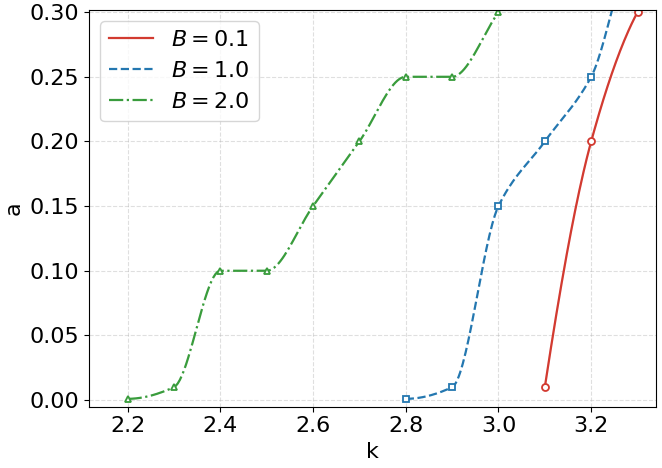
\includegraphics[width=\linewidth]{figures/chap2/initial_c_B_varies_.png}
		\caption{}
		\label{fig:B_varies_different_ic}
	\end{subfigure}
	\hfill
	\begin{subfigure}[t]{0.48\textwidth}
		\centering
		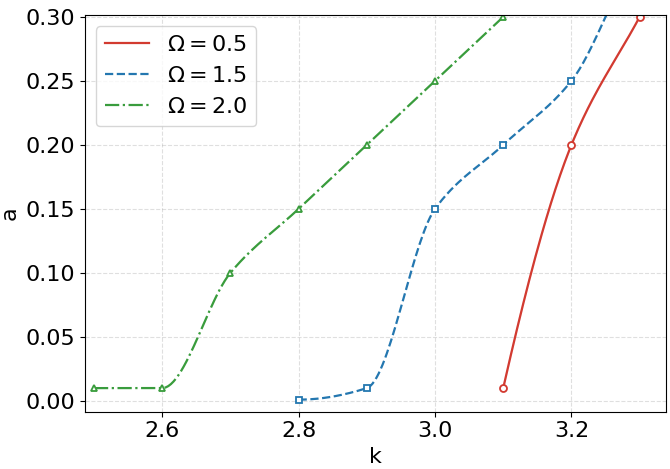
\includegraphics[width=\linewidth]{figures/chap2/initial_c_Omega_varies_.png}
		\caption{}
		\label{fig:Omega_varies_different_ic}
	\end{subfigure}
	\vspace{0.6cm}
	\begin{subfigure}[t]{0.48\textwidth}
		\centering
		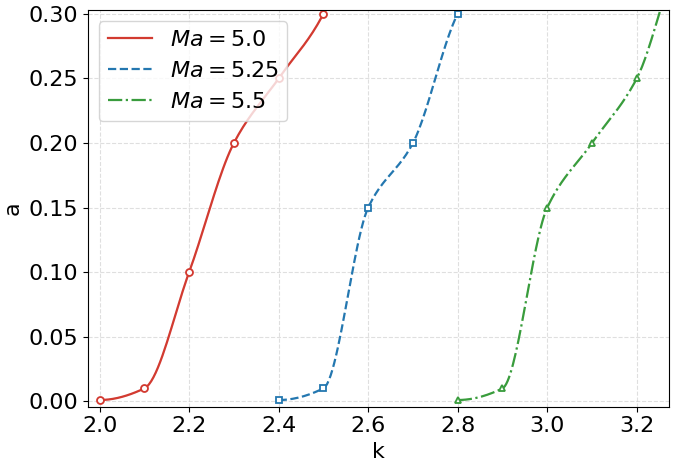
\includegraphics[width=\linewidth]{figures/chap2/initial_c_Ma_varies_.png}
		\caption{}
		\label{fig:Ma_varies_different_ic}
	\end{subfigure}
	
	\caption{
		Влияние амплитуды начального возмущения на устойчивость пленки:
		(a) изменение амплитуды внешнего воздействия $\mathrm{B}$
		($\mathrm{Ma}=5.5,\ \Omega=1.5$);
		(б) изменение частоты внешнего воздействия $\Omega$
		($\mathrm{B}=1.0,\ \mathrm{Ma}=5.5$);
		(в) изменение числа Марангони $\mathrm{Ma}$
		($\mathrm{B}=1.0,\ \Omega=1.5$).
		Остальные параметры имеют значения:
		$\mathrm{Ca}=2.5$,
		$\mathrm{G}=3.0$,
		$\mathrm{Pr}=7.0$,
		$\beta=1$.
	}
	\label{fig:different_initial_conditions_thermal}
\end{figure}

%Следует подчеркнуть, что такой анализ невозможно провести в рамках линейной теории устойчивости, поскольку амплитуда начального возмущения не входит в линеаризованные уравнения, определяющие динамику системы.

Нейтральные кривые на рис.~\ref{fig:different_initial_conditions_thermal} разделяют области устойчивости и неустойчивости. Области неустойчивости расположены слева от соответствующих нейтральных кривых. Увеличение амплитуды начального возмущения дестабилизирует систему, тогда как увеличение волнового числа расширяет область устойчивости. Увеличение интенсивности внешних вибраций (амплитуды или частоты воздействия) смещает критическое волновое число в сторону меньших значений (рис. \ref{fig:B_varies_different_ic}, \ref{fig:Omega_varies_different_ic}), тогда как усиление нагрева смещает его в сторону больших значений, способствуя образованию капиллярных волн  (рис. \ref{fig:Ma_varies_different_ic}). 

Эти результаты согласуются с результатами, полученными в рамках линейного анализа устойчивости.

\subsubsection{Карты устойчивости для различных чисел Марангони и в условиях микрогравитации и невесомости}

Была решена полная нелинейная задача и построены карты устойчивости в плоскости параметров $\mathrm{B},\Omega$ для двух варьируемых параметров. В первом случае варьировалось число Марангони при фиксированных остальных параметрах. Во втором случае варьировалось число Галилея для исследования условий микрогравитации ($\mathrm{G}=1.0$ и $\mathrm{G}=2.0$) и невесомости ($\mathrm{G}=0.0$).

Начальное возмущение задавалось в соответствии с уравнением \eqref{eq:perturb_profiles_thermal}, где $a=0.01$ и $k=2.0$.

\begin{figure}
	\centering
	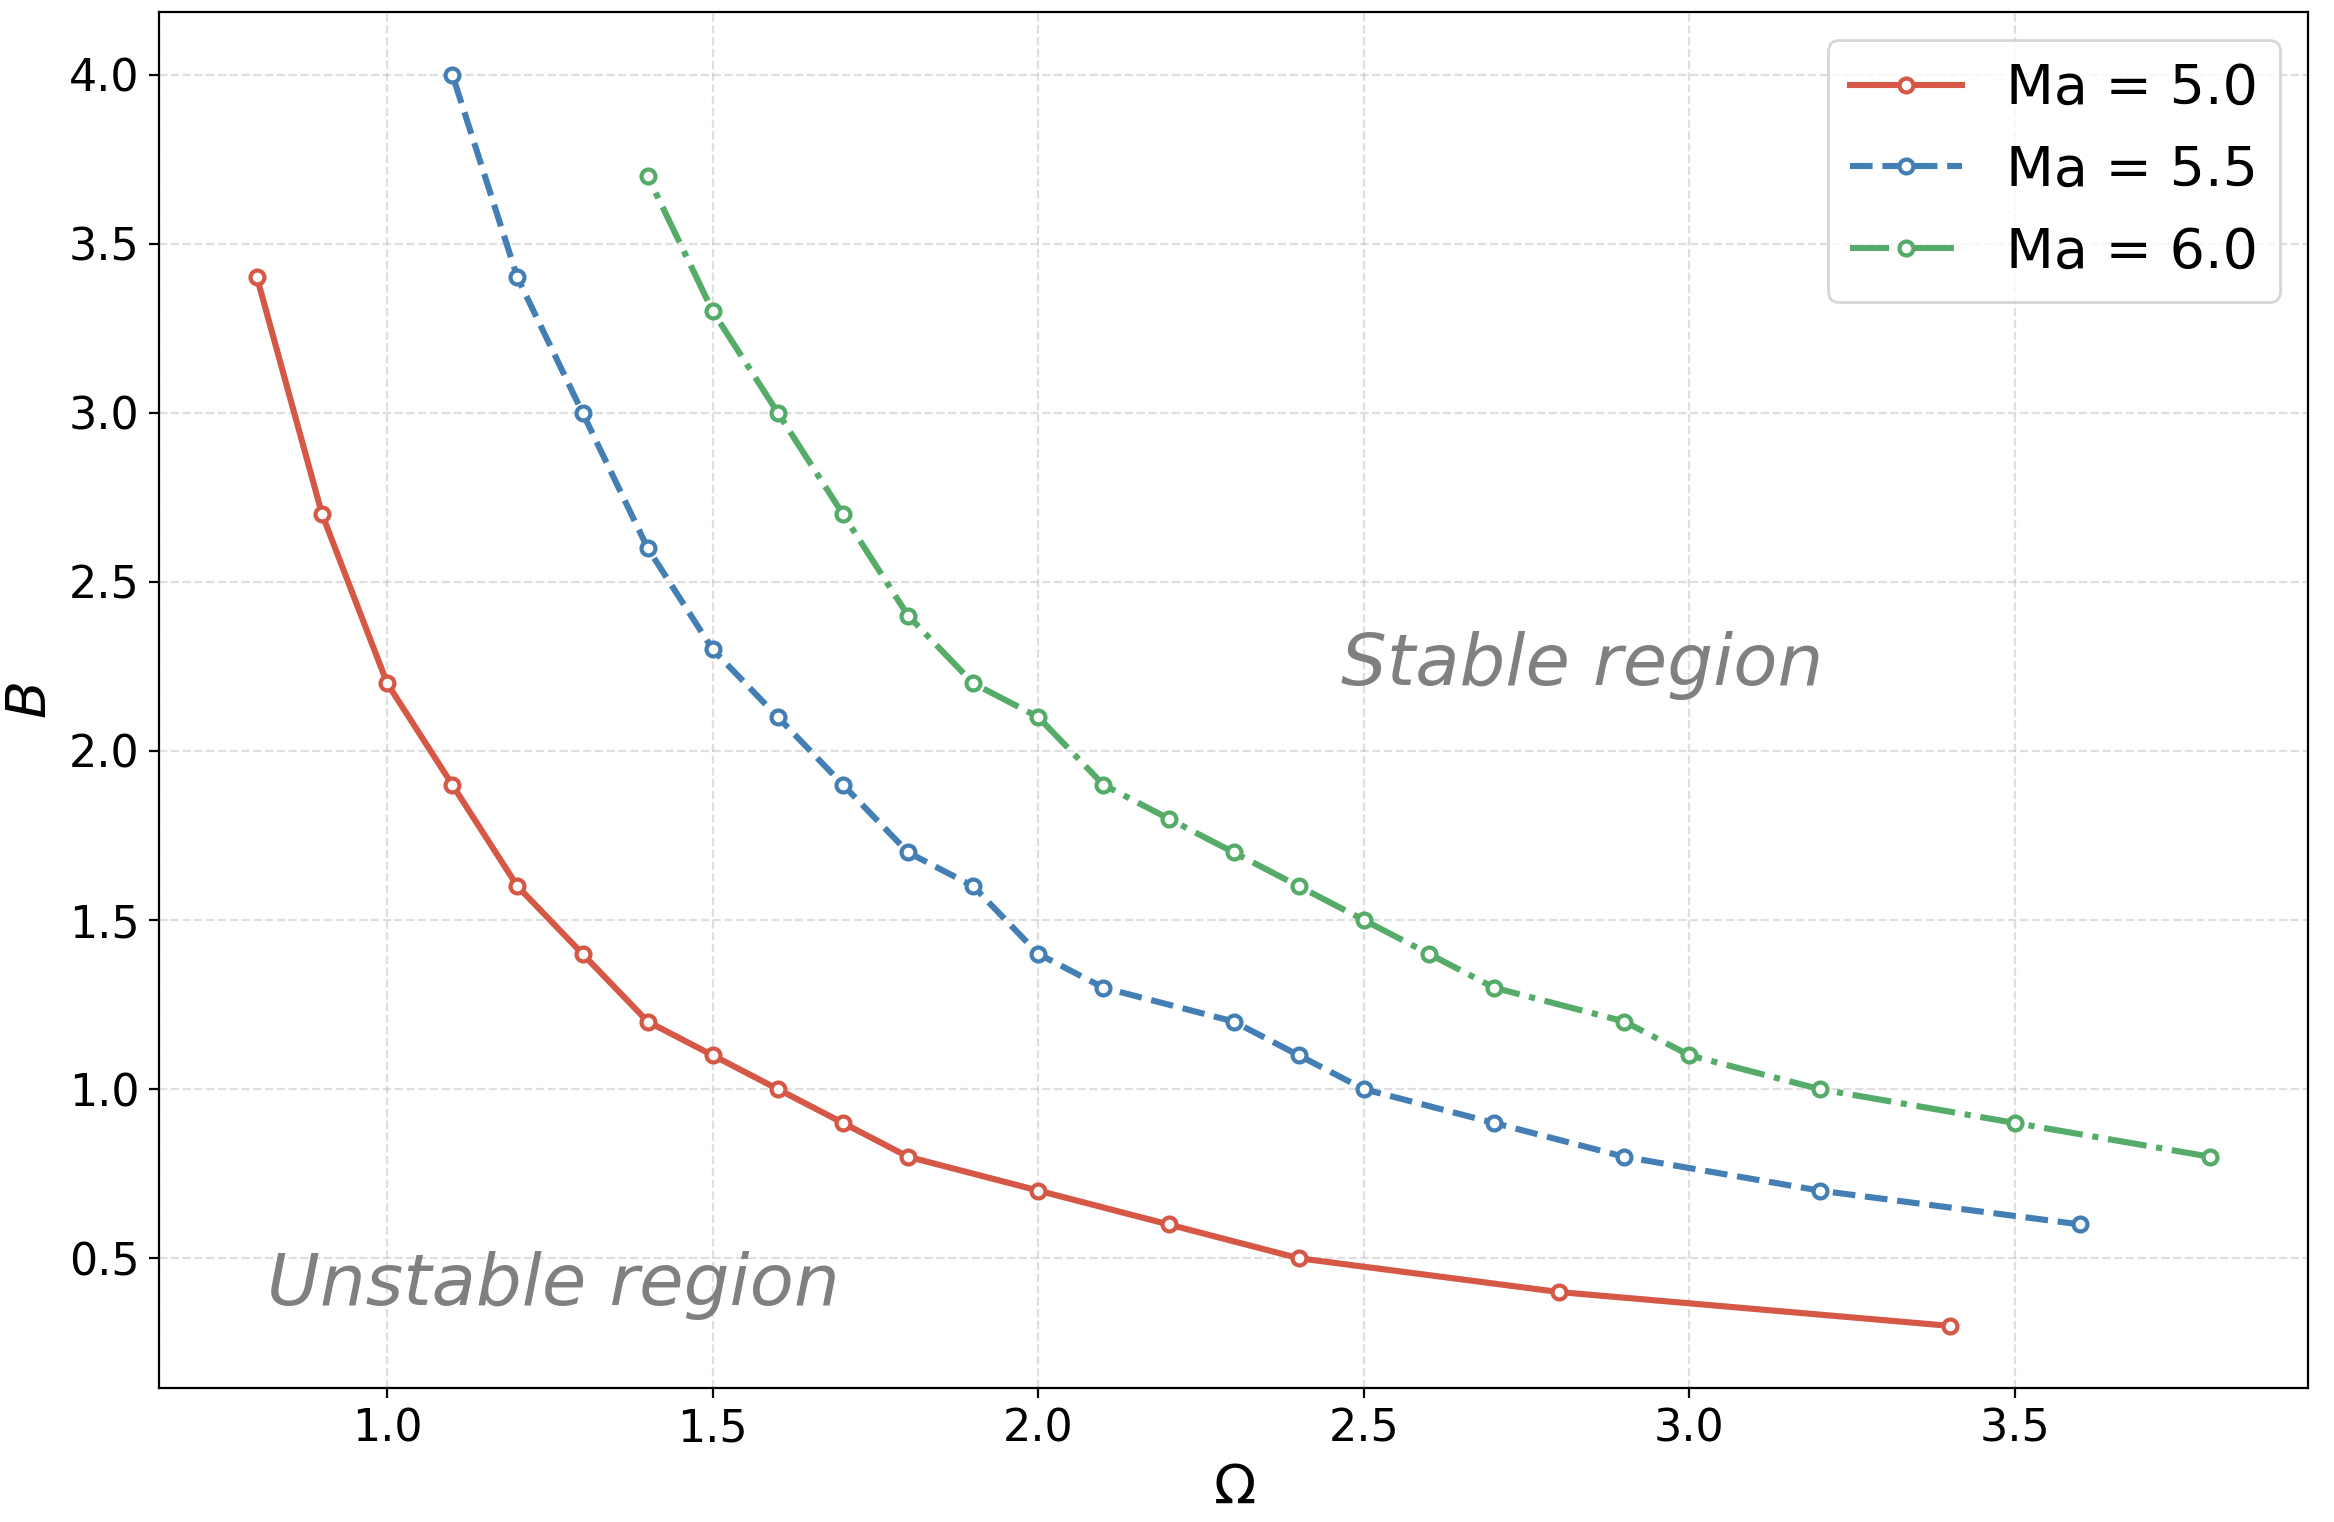
\includegraphics[width=0.79\linewidth]{figures/chap2/different_Ma_4.png}
	\caption{Кривые нейтральной устойчивости для различных значений числа Марангони. Остальные параметры имеют значения:
		$\mathrm{Ca}=2.5$,
		$\mathrm{G}=3.0$,
		$\mathrm{Pr}=7.0$,
		$\mathrm{\beta}=1$.}
	\label{fig:different_Ma_thermal}
\end{figure}

\begin{figure}
	\centering
	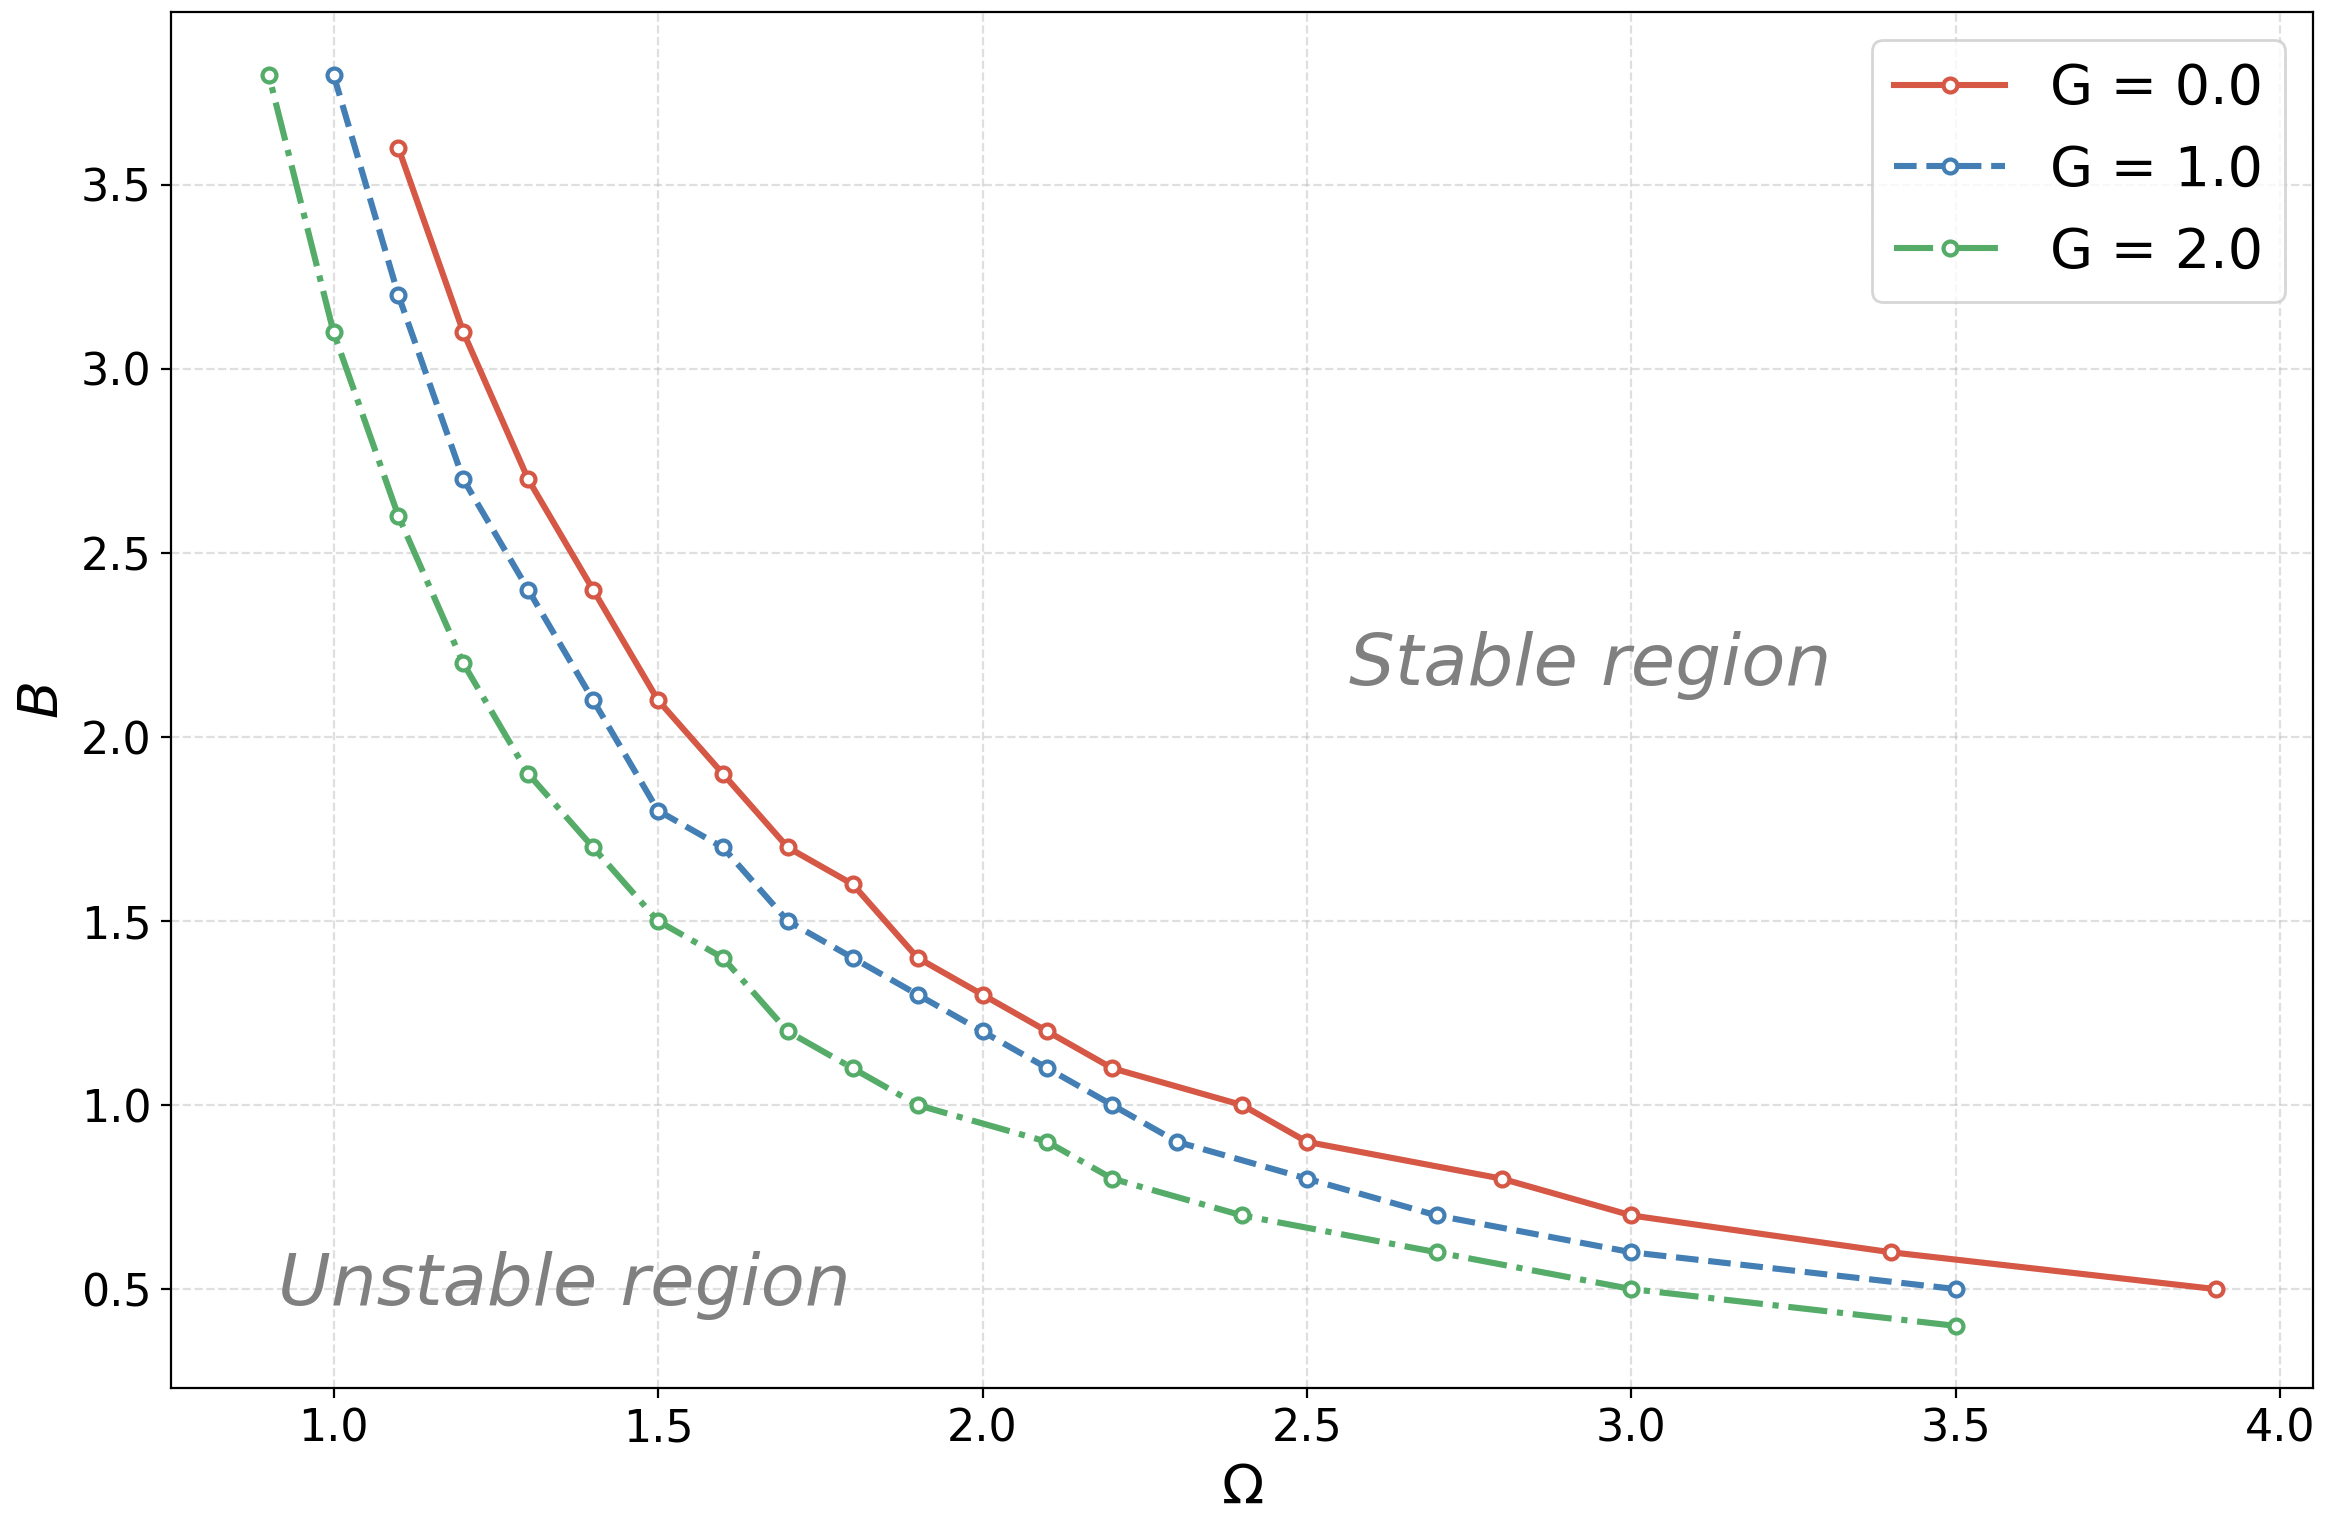
\includegraphics[width=0.79\linewidth]{figures/chap2/different_G_2.png}
	\caption{Кривые нейтральной устойчивости для различных значений числа Галилея. Остальные параметры имеют значения:
		$\mathrm{Ca}=2.5$,
		$\mathrm{Ma}=5.0$,
		$\mathrm{Pr}=7.0$,
		$\mathrm{\beta}=1$.}
	\label{fig:different_G_thermal}
\end{figure}

Всего было выполнено около 4500 численных расчетов. Амплитуда вибрационного воздействия варьировалась от 0 до 4 с шагом 0.1, тогда как частота вибраций изменялась от 0.5 до 4 с тем же шагом. На этапе постобработки для каждого значения управляющего параметра определялась граница устойчивости, после чего полученные граничные точки использовались для построения нейтральных кривых посредством интерполяции. Соответствующие карты устойчивости представлены на рис.~\ref{fig:different_Ma_thermal}--\ref{fig:different_G_thermal}.

Как видно из этих графиков, увеличение числа Марангони приводит к уменьшению области устойчивости, что свидетельствует о дестабилизирующем воздействии нагрева на систему (рис. \ref{fig:different_Ma_thermal}). Напротив, гравитация оказывает стабилизирующее воздействие (рис. \ref{fig:different_G_thermal}). Тем не менее результаты показывают, что вибрационная стабилизация остается возможной даже в невесомости.

\subsection{Слабонелинейный анализ}\label{subsection:weakly_nonlinear_thermo}

Проведем слабонелинейный анализ динамических уравнений  \eqref{eq:avrged_Ma_first_thermal}--\eqref{eq:avrged_Ma_second_thermal}. Для этого разложим координату поверхности раздела и температуру на свободной границе в ряд по малому параметру:
\begin{align}
	\bar{\xi} &= 1 + \varepsilon\xi_1 + \varepsilon^2\xi_2 + O(\varepsilon^3), \\
	\bar{T} &= 1 + \varepsilon T_1 + \varepsilon^2 T_2 + O(\varepsilon^3).
\end{align}
Аналогичным образом раскладывается производная по времени:
\begin{equation}
	\frac{\partial}{\partial t} =
	\frac{\partial}{\partial t_0}
	+ \varepsilon\frac{\partial}{\partial t_1}
	+ \varepsilon^2\frac{\partial}{\partial t_2}
	+ O(\varepsilon^3).
\end{equation}

Как и следует ожидать, в нулевом порядке по $\varepsilon$ получаются результаты линейной теории. Первый порядок не дает поправок к полученным результатам, тогда как уравнения второго порядка принимают вид:
\begin{align}
	\frac{\partial\xi_1}{\partial t_2} &= \frac{\partial}{\partial X}\left(\frac{\partial\Pi^{(1)}}{\partial X}\xi_1^2 
	+ \frac{\partial\Pi^{(2)}}{\partial X}\xi_1 + \frac{1}{3}\Pi^{(3)} \right.  \left. + \frac{\mathrm{Ma}}{2}\xi_1^2\left(\frac{\partial T_1}{\partial X} - \frac{\partial\xi_1}{\partial X}\right)\right)
	\nonumber \\
	&\quad - \frac{\mathrm{B}^2\Omega^2}{2}\left(R_1\left(\frac{\partial\xi_1}{\partial X}\right)^3 
	+ R_2\frac{\partial\xi_1}{\partial X}\xi_1\frac{\partial^2\xi_1}{\partial X^2}\right),
\end{align}
\begin{align}
	\frac{\partial T_1}{\partial t_2} &= -\frac{\beta}{\mathrm{Pr}} f_1   + \left(\xi_1\frac{\partial\Pi^{(1)}}{\partial X} 
	+ \mathrm{Ma}\xi_1\frac{\partial f_1}{\partial X}\right)\frac{\partial f_1}{\partial X} + \frac{\partial}{\partial X}\left(\frac{3}{4}\xi_1^2\frac{\partial\Pi^{(1)}}{\partial X} 
	+ \frac{\xi_1}{2}\frac{\partial\Pi^{(2)}}{\partial X} \right. \nonumber \\
	&\quad \left. + \frac{1}{3}\Pi^{(3)} + \frac{\mathrm{Ma}}{2}\xi_1^2\frac{\partial f_1}{\partial X}\right).
\end{align}
где:
\begin{align*}
	\Pi^{(1)} &= \mathrm{G}\xi_1 - \mathrm{Ca}\frac{\partial^2\xi_1}{\partial X^2} - \frac{\mathrm{B}^2\Omega^2}{2}m_1\frac{\partial\xi_1}{\partial X}, \\
	\Pi^{(2)} &= \mathrm{G}\xi_2 - \frac{\mathrm{B}^2\Omega^2}{2}\left((1-m_1)\xi_1\frac{\partial\xi_1}{\partial X} + \right. \left. \xi_1\frac{\partial\xi_1}{\partial X}m_2\right), \\
	\Pi^{(3)} &= \frac{\mathrm{B}^2\Omega^2}{2}m_3, f_1=T_1-\xi_1,
\end{align*}
\begin{align*}
	R_1 = 3\frac{4\sinh(\gamma_0)\sin(\gamma_0) - \gamma_0(\psi_+^0\phi_+^0 - \psi_-^0\phi_-^0)}{2\gamma_0^2(\psi_+^0)^2}, \\
	R_2 = -\frac{1}{3} + \frac{11\phi_-^0 - 3\gamma_0\psi_-^0}{\gamma_0^3\psi_+^{0}},
\end{align*}
\begin{align*}
	\psi_+^0 = \cosh(\gamma_0) + \cos(\gamma_0), \\ 
	\psi_-^0 = \cosh(\gamma_0) - \cos(\gamma_0), \\ 
	\phi_+^0 = \sinh(\gamma_0) + \sin(\gamma_0), \\ 
	\phi_-^0 = \sinh(\gamma_0) - \sin(\gamma_0), \\
	\gamma_0= \sqrt{2\Omega}.
\end{align*}
\begin{equation*}
	m_1 = 1 - \frac{2}{ \gamma_0} \frac{(\sin \gamma_0 + \sinh \gamma_0)}{(\cos \gamma_0 + \cosh \gamma_0)},
\end{equation*}
\begin{equation*}
	m_2 = \frac{\sinh^2 \gamma_0 - \sin^2 \gamma_0}{(\cos \gamma_0 + \cosh \gamma_0)^2},
\end{equation*}
\begin{equation*}
	m_3= \frac{\sqrt{2}}{2 (\cosh\gamma_0+\cos\gamma_0)^3}
	\Big[\xi_1^2  \frac{\partial \bar{\xi_1}}{\partial X} N_1+N_2\Big],
\end{equation*}
\begin{equation*}
	\begin{aligned}
		N_1={}&
		\sqrt{2}\gamma_0(\cos\gamma_0+1)
		\Big[\sinh\gamma_0
		(1-\cos\gamma_0+\cosh\gamma_0)\\
		&\quad+\sin\gamma_0(1-\cosh\gamma_0)\Big]
		+\frac{3}{2}\gamma_0\sinh^2\gamma_0\sin\gamma_0\\
		&\quad-\sinh^3\gamma_0
		+4\sqrt{2}\gamma_0
		\left(\cosh\frac{\gamma_0}{2}
		-\sin\frac{\gamma_0}{2}\right).
	\end{aligned}
\end{equation*}
\begin{equation*}
	N_2=\sqrt{2}\gamma_0\sin\gamma_0\left[3(\cosh\gamma_0-1)\,\cosh\frac{\gamma_0}{2} - \cos\gamma_0 - 1\right].
\end{equation*}


Как хорошо известно, результат слабонелинейного анализа дает поправку к результатам линейного анализа устойчивости и позволяет понять и уточнить поведение системы в окрестности порога неустойчивости.

Полученная система уравнений второго порядка была численно проинтегрирована с использованием указанного выше решателя. Уточнение результатов по сравнению с линейным анализом устойчивости (см. рис.~\ref{fig:linear_stability_thermal}) заключается в том, что при $\mathrm{B}=0.10$ и $\mathrm{B}=1.0$ решение остается устойчивым во всем диапазоне критических волновых чисел, тогда как при $\mathrm{B}=2.0$ оно становится неустойчивым.

\subsection{Выводы по главе}

В данной главе исследована динамика тонкой жидкой пленки при одновременном нагреве снизу и вертикальных вибрациях. Поставленная задача была разделена на пульсационную систему и осредненную систему уравнений. Пульсационная система уравнений была решена аналитически. Осредненная система уравнений, с учетом вклада пульсационных слагаемых, была преобразована к динамической системе двух уравнений. 

Проведен линейный анализ устойчивости свободной границы. Показано, что капиллярные и гравитационные силы оказывают стабилизирующее воздействие, вертикальный градиент температуры вносит дестабилизирующее воздействие. Вертикальные вибрации способны подавить развивающуюся неустойчивость. 

Динамическая система нелинейных уравнений была проинтегрирована численно методом Radau IIA. Показано, что нелинейная динамика зависит от амплитуды начального возмущения. Достаточно большие возмущения способны приводить к развитию неустойчивости в областях, линейно устойчивых при малых возмущениях. Увеличение волнового числа, напротив, способствует стабилизации свободной поверхности. Построены карты устойчивости для различных значений параметров. Установлено, что увеличение числа Марангони приводит к уменьшению области устойчивости. Показано также, что даже в условиях невесомости стабилизация может быть достигнута за счет вибрационного воздействия.

Проведен слабонелинейный анализ, уточняющий результаты линейной теории с учетом эффектов конечной амплитуды вблизи порога неустойчивости. Установлено, что нелинейные поправки изменяют границу устойчивости: при малых амплитудах внешних вибраций критический порог увеличивается, тогда как при относительно больших он уменьшается.

Дальнейшим направлением развития данной задачи является переход к трехмерной постановке, а также более подробный слабонелинейный анализ, направленный на описание волновых структур, возникающих на свободной поверхности, и определение типа бифуркации. Кроме того, может быть исследовано влияние различных типов начальных возмущений, в том числе возмущений со сдвигом фаз.

\mychapter{3}{Динамика тонкого слоя магнитной жидкости в стационарном магнитном поле под воздействием вертикальных вибраций}{chap:ferro}


Данная глава посвящена аналитическому исследованию динамики тонкого слоя магнитной жидкости  под воздействием вертикальных вибраций в вертикальном магнитном поле. Метод решения включает в себя разделение полной системы уравнений на пульсационные и осредненные поля. 

Найдено решение для пульсационных компонент, получено распределение магнитного поля при малых отклонениях поверхности раздела. Решена линейная задача устойчивости тонкой пленки.  

Результаты опубликованы в работах \cite{Volodin2021ferro, Alabuzhev2022}.

\subsection{Система уравнений феррожидкости со свободной границей под действием вибраций}

Рассматривается динамика тонкой, бесконечной в продольном направлении вязкой, несжимаемой пленки магнитной жидкости, расположенной на плоской горизонтальной твердой подложке, $c_0$ -- толщина пленки в невозмущенном состоянии (см. рис. \ref{fig:problem_statement_ferro}). Верхняя поверхность пленки свободна и деформируема, над ней находится невесомый газ. На систему действует вертикальное стационарное магнитное поле $\mathbf{H}(0, H_0)$. Подложка является немагнитной и совершает вертикальные гармонические колебания с частотой $\omega$ и амплитудой $b$.

Внутри феррожидкости отсутствуют свободные электрические заряды, магнитные частицы распределены однородно. Время релаксации магнитного поля таково, что оно мгновенно успевает подстраиваться под вибрационное воздействие. Задача рассматривается в изотермической постановке. 

%Цифрами на рисунке обозначены номера сред, которые далее будут обозначаться нижними индексами.

\begin{figure}
	\centering
	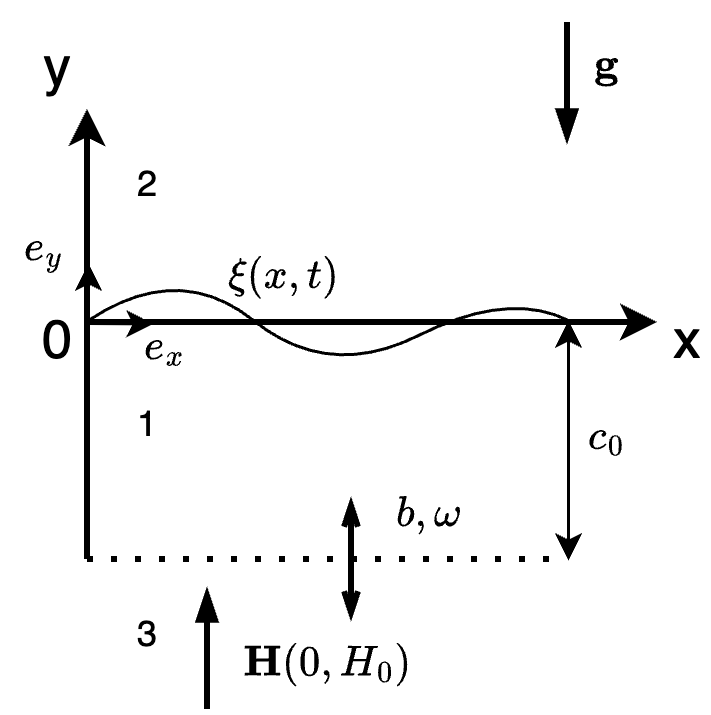
\includegraphics[width=0.45\linewidth]{figures/chap3/problem_statement.png}
	\caption{Геометрия задачи. Обозначения сред: 1 -- магнитная жидкость, 2 -- невесомый газ над свободной поверхностью, 3 -- среда под твердой подложкой.}
	\label{fig:problem_statement_ferro}
\end{figure}


Система уравнений феррогидродинамики в случае стационарного магнитного поля имеет вид \cite{Cowley1989, Berkovskiy1989, Kirko2019}:
\begin{equation}
	\nabla \cdot \mathbf{v} = 0,
\end{equation}
\begin{equation}
	\rho\left(
	\frac{\partial \mathbf{v}}{\partial t}
	+(\mathbf{v} \cdot \nabla)\mathbf{v}
	\right)
	=
	-\nabla p
	+\eta\Delta\mathbf{v}
	+\mathbf{f},
\end{equation}
\begin{equation}
	\nabla \cdot \mathbf{B} = 0,
\end{equation}
\begin{equation}
	\nabla \times \mathbf{H} = 0,
\end{equation}
где $\mathbf{v} = (u,v)$ -- скорость жидкости, $p$ -- поле давления, $\rho$ -- плотность жидкости, $\eta=\rho \nu$ -- коэффициент динамической вязкости жидкости, $\nu$ -- коэффициент кинематической вязкости жидкости, $\mathbf{H}$ -- напряженность магнитного поля, $\mathbf{B} $ -- индукция магнитного поля, $\mu_0$ -- магнитная постоянная, $\mathbf{f}$ -- внешняя сила, включающая гравитационный вклад и вклад магнитного поля, $\nabla$ -- векторный дифференциальный оператор первого порядка, $\Delta$ -- скалярный дифференциальный оператор второго порядка.

Для удобства перейдем в неинерциальную систему отсчета, связанную с подложкой. Внешняя сила $\mathbf{f}$ в этом случае должна быть записана следующим образом:
\begin{equation} \label{eq:ext_force_ferro}
	\mathbf{f}
	=
	\mu_0(\mathbf{M} \cdot \nabla)\mathbf{H}
	-
	\rho g \mathbf{e}_y
	-
	\rho b \omega^2 \sin(\omega t)\mathbf{e}_y,
\end{equation}
где $\mathbf{M}$ --- вектор намагниченности. 

Вектор намагниченности зависит от напряженности магнитного поля
внутри феррожидкости ($\mathbf{H}_1$):
\begin{equation*}
	\mathbf{M} = \chi(\mathbf{H}_1)\mathbf{H}_1,
\end{equation*}
где $\chi(\mathbf{H}_1)$ --- магнитная восприимчивость. Для изотропного магнетика без гистерезиса в умеренных полях, можно считать $\chi(\mathbf{H}_1)$ константой $\sim 1$~\cite{Berkovskiy1989, Korovin2013}.

Первое слагаемое в (\ref{eq:ext_force_ferro}) можно переписать в более удобном виде. Так как 
\begin{equation*}
   ( \mathbf{H} \cdot \nabla   )\mathbf{H} = \frac{1}{2} \nabla(\mathbf{H}\mathbf{H}) - \mathbf{H} \times (\nabla \times \mathbf{H}),
\end{equation*}
то с учетом определения вектора намагниченности и уравнения напряженности магнитного поля, получим:
\begin{equation*}
	\mu_0(\mathbf{M} \cdot \nabla)\mathbf{H}
	=
	\mu_0|\mathbf{M}||\nabla\mathbf{H}|.
\end{equation*}

Тензор напряжений с учетом магнитостатического вклада для несжимаемой среды в индексной форме записи имеет вид \cite{Cowley1989, Berkovskiy1989}: 

\begin{equation}\label{eq:viscous_ferro}
	\sigma_{ik}
	=
	p\delta_{ik}
	-
	\eta
	\left(
	\frac{\partial v_i}{\partial x_k}
	+
	\frac{\partial v_k}{\partial x_i}
	\right)
	+
	\frac{1}{2}\mu_0 H^2\delta_{ik}
	-
	H_i B_k.
\end{equation}

Запишем граничные условия для рассматриваемой задачи. 

На подложке $y=-c_0$ должны выполняться условия прилипания для обеих компонент скорости, отсутствие скачка тангенциальных компонент напряженности магнитного поля и отсутствие
скачка нормальных компонент индукции магнитного поля:
\begin{equation}
		u = v = 0, 
\end{equation}
\begin{equation}
		H_{1x} = H_{3x}, 
\end{equation}
\begin{equation}
		B_{1y} = B_{3y},
\end{equation}
где нижними индексами обозначены номера сред (см. рис. \ref{fig:problem_statement_ferro}).

На свободной поверхности $y=\xi(x,t)$ должны удовлетворяться
кинематическое условие для скорости, баланс тангенциальных и нормальных
напряжений для тензора напряжений с учетом магнитного скачка
давления (см. \eqref{eq:viscous_normal_bc_thermal}--\eqref{eq:viscous_tangential_bc_thermal} с учетом \eqref{eq:viscous_ferro}) и отсутствие скачка нормальной и тангенциальной составляющих
векторов $\mathbf{B}$ и $\mathbf{H}$, соответственно:
\begin{equation}
	\frac{\partial \xi}{\partial t}
	+
	u\frac{\partial \xi}{\partial x}
	=
	v,
\end{equation}
\begin{equation}
	\left(
	1-
	\left(
	\frac{\partial \xi}{\partial x}
	\right)^2
	\right)
	\left(
	\frac{\partial u}{\partial y}
	+
	\frac{\partial v}{\partial x}
	\right)
	+
	2\frac{\partial \xi}{\partial x}
	\left(
	\frac{\partial v}{\partial y}
	-
	\frac{\partial u}{\partial x}
	\right)
	=
	0,
\end{equation}

\begin{equation}
	\begin{aligned}
		p
		&=
		-\varphi
		+
		\frac{2\rho\nu}
		{1+\left(\dfrac{\partial \xi}{\partial x}\right)^2}
		\left\{
		\frac{\partial u}{\partial x}
		\left[
		\left(
		\frac{\partial \xi}{\partial x}
		\right)^2
		-1
		\right]
		-
		\left(
		\frac{\partial u}{\partial y}
		+
		\frac{\partial v}{\partial x}
		\right)
		\frac{\partial \xi}{\partial x}
		\right\}
		\\
		&\quad
		-
		\frac{\alpha \dfrac{\partial^2 \xi}{\partial x^2}}
		{\left(
			1+
			\left(
			\dfrac{\partial \xi}{\partial x}
			\right)^2
			\right)^{3/2}}
		-
		\frac{\mu_0}
		{2\left(
			1+
			\left(
			\dfrac{\partial \xi}{\partial x}
			\right)^2
			\right)}
		\left(
		M_y
		-
		M_x
		\frac{\partial \xi}{\partial x}
		\right)^2,
	\end{aligned}
\end{equation}
\begin{equation}
	(H_{1x}-H_{2x})\tau_x
	+
	(H_{1y}-H_{2y})\tau_y
	=
	0,
\end{equation}
\begin{equation}
	(B_{1x}-B_{2x})n_x
	+
	(B_{1y}-B_{2y})n_y
	=
	0,
\end{equation}
где $M_x$, $M_y$ означают $x$- и $y$-компоненты вектора намагниченности,
$\varphi$ --- притягивающий потенциал сил Ван-дер-Ваальса, которым в дальнейшем будем пренебрегать (см. раздел \ref{sec:governing_params_estimation_thermal}). 

Обезразмерим исходную задачу, выбрав за единицы измерения
расстояния, времени, скорости, давления и характерного значения
напряженности магнитного поля, следующие величины: $c_0$, $c_0^2/\nu$, $\nu/ c_0$,
$\rho\nu^2/c_0^{2}$, $H_0$, соответственно.


Получаем для тонкого слоя магнитной жидкости следующую систему
уравнений в безразмерном виде:
\begin{equation}\label{eq:div_ferro}
\frac{\partial u}{\partial x}
+
\frac{\partial v}{\partial y}
=0,
\end{equation}
\begin{equation}
\frac{\partial u}{\partial t}
+
\left(
u\frac{\partial}{\partial x}
+
v\frac{\partial}{\partial y}
\right)u
=
-\frac{\partial p}{\partial x}
+
\left(
\frac{\partial^2}{\partial x^2}
+
\frac{\partial^2}{\partial y^2}
\right)u
+
\mathrm{Ha}
\left(
H_x\frac{\partial}{\partial x}
+
H_y\frac{\partial}{\partial y}
\right)H_x,
\end{equation}
\begin{equation}
	\begin{aligned}
		\frac{\partial v}{\partial t}
		+
		\left(
		u\frac{\partial}{\partial x}
		+
		v\frac{\partial}{\partial y}
		\right)v
		&=
		-\frac{\partial p}{\partial y}
		+
		\left(
		\frac{\partial^2}{\partial x^2}
		+
		\frac{\partial^2}{\partial y^2}
		\right)v
		\\
		&\quad
		+ \mathrm{Ha}
		\left(
		H_x\frac{\partial}{\partial x}
		+
		H_y\frac{\partial}{\partial y}
		\right)H_y
		- \mathrm{G}
		- \mathrm{B}^{*}\Omega^2\sin(\Omega t),
	\end{aligned}
\end{equation}
\begin{equation}
\frac{\partial B_x}{\partial x}
+
\frac{\partial B_y}{\partial y}
=0,
\end{equation}
\begin{equation}
\frac{\partial H_y}{\partial x}
-
\frac{\partial H_x}{\partial y}
=0.
\end{equation}

Граничные условия на подложке (\(y=-1\)):
\begin{equation}
u=v=0,
\end{equation}
\begin{equation}
H_{1x}=H_{3x},
\end{equation}
\begin{equation}
B_{1y}=B_{3y}.
\end{equation}

На свободной границе \(y=\xi(x,t)\):
\begin{equation}
\frac{\partial \xi}{\partial t}
+
\left(
u\frac{\partial}{\partial x}
\right)\xi
=
v,
\end{equation}

\begin{equation}
\left(
1-
\left(\frac{\partial \xi}{\partial x}\right)^2
\right)
\left(
\frac{\partial u}{\partial y}
+
\frac{\partial v}{\partial x}
\right)
+
2\frac{\partial \xi}{\partial x}
\left(
\frac{\partial v}{\partial y}
-
\frac{\partial u}{\partial x}
\right)
=0,
\end{equation}
\begin{equation}\label{eq:bc_free_surface_ferro}
	\begin{aligned}
		p
		&=
		\frac{1}
		{1+\left(\frac{\partial \xi}{\partial x}\right)^2}
		\Bigg\{
		\frac{\partial u}{\partial x}
		\left[
		\left(\frac{\partial \xi}{\partial x}\right)^2-1
		\right]
		\\
		&\quad
		-
		\left(
		\frac{\partial u}{\partial y}
		+
		\frac{\partial v}{\partial x}
		\right)
		\frac{\partial \xi}{\partial x}
		\Bigg\}
		-
		\frac{
			\mathrm{Ca^*}\dfrac{\partial^2\xi}{\partial x^2}
		}{
			\left[
			1+
			\left(\dfrac{\partial \xi}{\partial x}\right)^2
			\right]^{3/2}
		}
		\\
		&\quad
		-
		\frac{\chi\cdot \mathrm{Ha}}
		{
			2\left[
			1+
			\left(\dfrac{\partial \xi}{\partial x}\right)^2
			\right]
		}
		\left(
		H_y-H_x\frac{\partial \xi}{\partial x}
		\right)^2.
	\end{aligned}
\end{equation}

В вышеописанную систему входят следующие безразмерные параметры:
\[
\mathrm{Ca^*} = \frac{\alpha c_0}{\rho \nu^2},
\qquad
\mathrm{G} = \frac{g c_0^3}{\nu^2},
\qquad
\mathrm{B}^* = \frac{b}{c_0},
\qquad
\Omega = \frac{c_0^2}{\nu}\omega,
\qquad
\mathrm{Ha} = \frac{\mu_0 \chi c_0^2 H_0^2}{\rho \nu^2},
\]
где \(\mathrm{Ca^*}\) --- капиллярное число, \(\mathrm{G}\) --- число Галилея, 
\(\mathrm{B}^*\) --- безразмерная амплитуда колебаний, 
\(\Omega\) --- безразмерная частота колебаний, \(\mathrm{Ha}\) имеет смысл 
безразмерного параметра отношения магнитных сил к инерционным. 

Оценим характерные значения безразмерных параметров. Рассмотрим слой жидкости толщиной \(c_0 \sim 10^{-4}\,\text{м}\), характерное значение приложенного поля \(H_0 \sim 10^4\,\text{А/м}\), другие характеристики системы:  \(\mu_0 = 4 \pi \cdot10^{-7}\,\text{Н/А}^2\), \(\chi \sim 1\), \(\rho = 1400\,\text{кг/м}^3\), $\alpha = 25 \cdot 10^{-3}~\text{Н/м},$ \(\nu =10^{-6}\,\text{м}^2/\text{с}\), $b=10^{-3}$, $\omega=100$ рад/c. Тогда значения безразмерных параметров: $\mathrm{Ca^*} \sim 2 \cdot 10^3, \mathrm{G} \sim 10, \mathrm{B}^{*} \sim 10, \Omega \sim 1, \mathrm{Ha} \sim 9 \cdot 10^2$. 

В дальнейшем будем рассматривать асимптотическое приближение, в котором капиллярное число и амплитуда колебаний считаются большими (как в предыдущей главе):
\begin{equation}\label{eq:scaled_Ca_B_ferro}
	\mathrm{Ca^*}=\varepsilon^{-2}\mathrm{Ca},\qquad
	\mathrm{B^*}=\varepsilon^{-1}\mathrm{B},
\end{equation}
а остальные параметры не масштабируются.

\subsection{Метод решения}

Метод решения задачи аналогичен рассмотренному в предыдущей главе. Вводятся перемасштабированные переменные и иерархия временных масштабов (см. \eqref{eq:stretched_x_y_vars_thermal}--\eqref{eq:stretched_velocity_eq_thermal}, \eqref{eq:timescale_hierarchy_thermal}--\eqref{eq:time_derivative_expansion_thermal}). Полная система уравнений представляется в виде суммы пульсационных и осредненных полей (аналогично (\ref{eq:pressure_expansion_thermal})--(\ref{eq:interface_expansion_thermal})).
Считается, что магнитное поле мгновенно подстраивается под
вибрационное воздействие и поэтому пульсационная часть у него отсутствует:
\begin{equation}\label{eq:magnetic_field_split_ferro}
	\mathbf{H} = H_0 \mathbf{e_y} + \bar{ \mathbf{h}}
\end{equation}

В результате такой подстановки в безразмерную систему уравнений \eqref{eq:div_ferro}--\eqref{eq:scaled_Ca_B_ferro}, с учетом \eqref{eq:magnetic_field_split_ferro}, получим две системы уравнений. Одна описывает пульсационное течение, другая -- осредненное течение. 

Для замыкания задачи необходимо также найти распределение магнитного поля в случае отклонения поверхности раздела от равновесного состояния. 

\subsection{Распределение магнитного поля при малых отклонениях свободной границы} \label{sec:magnetic_field}

Прежде чем переходить к основной задаче, найдем распределение магнитного поля при слабых отклонениях границы раздела от равновесного состояния. 

Представим вектор напряженности магнитного поля в виде суммы двух полей:
\[
\mathbf{H}_k = \mathbf{H}_0^{(k)} + \overline{\mathbf{h}_k},
\]
где индекс $k=1,3$ обозначает номер среды (см. рис. \ref{fig:problem_statement_ferro}), $\mathbf{H}_0^{(k)}$ -- это распределение магнитного поля в случае недеформируемой границы,
$\overline{\mathbf{h}}_k$ -- это отклонение магнитного поля из-за деформации свободной границы.  

Из-за ориентации внешнего магнитного
поля и малого искривления поверхности, вектор $\overline{\mathbf{h}}_1$
слабо отклоняется от вертикали и можно считать, что внутри слоя
$x$--компонента $\overline{\mathbf{h}}_1$ много меньше
$y$--компоненты. Таким образом, внутри феррожидкости будем считать
$\overline{\mathbf{h}}_1(\varepsilon h_{1x},h_{1y})$.

Разложим $\overline{\mathbf{h}}_k$ в ряд по малому параметру:
\[
\overline{\mathbf{h}}_k =
\sum_{N=0}^{2} \varepsilon^N \mathbf{h}_k^{(N)}
+ O(\varepsilon^3)
\]
и запишем систему уравнений:
\[
\varepsilon^2
\frac{\partial h_{1x}^{(0)}}{\partial X}
+
\frac{\partial h_{1y}^{(0)}}{\partial Y}
=0,
\]
\[
\frac{\partial h_{1x}^{(0)}}{\partial Y}
-
\frac{\partial h_{1y}^{(0)}}{\partial X}
=0.
\]

\begin{align*}
	\frac{\partial h_{2,3x}^{(0)}}{\partial x} + \frac{\partial h_{2,3y}^{(0)}}{\partial y} &= 0, \\
	\frac{\partial h_{2,3x}^{(0)}}{\partial y} - \frac{\partial h_{2,3y}^{(0)}}{\partial x} &= 0.
\end{align*}
Заглавными буквами обозначены <<растянутые>> пространственные переменные внутри феррожидкости (см. (\ref{eq:stretched_x_y_vars_thermal})), строчными -- не перемасштабированные пространственные переменные в средах 2, 3 (см. рис.  \ref{fig:problem_statement_ferro}). 

Граничные условия на подложке запишутся следующим образом:
\begin{align*}
	h_{3x}^{(0)} &= h_{1x}^{(0)}, \\
	\mu_r h_{1y}^{(0)} &= 1 + h_{3y}^{(0)} - \mu_r H_0^{(1)},
\end{align*}
на свободной границе:
\begin{align*}
	\mu \left( H_0^{(1)} + h_{1y}^{(0)} \right) - \mu_0 \left( H_0^{(2)} + h_{2y}^{(0)} \right) &= \frac{\partial \xi}{\partial X} \left( \mu h_{1x}^{(0)} - \mu_0 h_{2x}^{(0)} \right), \\
	h_{1x}^{(0)} - h_{2x}^{(0)} &= \frac{\partial \xi}{\partial X} \left( 1 + h_{2y}^{(0)} - H_0^{(1)} - h_{1y}^{(0)} \right),
\end{align*}
где $\mu = \mu_0 \mu_r$ — магнитная проницаемость магнитной жидкости, $\mu_r = 1 + \chi$ — относительная магнитная проницаемость.

Решение данной задачи при $\xi = \zeta e^{ikX}$, где $\zeta$ -- мало, запишется в виде:
\begin{align}
	\mathbf{H}_1 &= i k \varepsilon^2 \left( \frac{\zeta M_0 (kY + \mu_r + k)}{2\mu_r + k} e^{ikX} \right) \mathbf{e}_x + \left( \frac{1}{\mu_r} + \varepsilon \frac{\zeta M_0 k}{2\mu_r + k} e^{ikX} \right) \mathbf{e}_y, \\
	\mathbf{H}_2 &= -i k \varepsilon \left( \frac{\mu_r \zeta M_0}{2\mu_r + k} e^{ikx - ky} \right) \mathbf{e}_x + \varepsilon k \left( \frac{\mu_r \zeta M_0}{2\mu_r + k} e^{ikx - ky} \right) \mathbf{e}_y, \\
	\mathbf{H}_3 &= i k \varepsilon \left( \frac{\mu_r \zeta M_0}{2\mu_r + k} e^{ikx + k(y+1)} \right) \mathbf{e}_x + \varepsilon k \left( \frac{\mu_r \zeta M_0}{2\mu_r + k} e^{ikx + k(y+1)} \right) \mathbf{e}_y,
\end{align}
где $M_0 = (\mu_r - 1) H_0^{(1)}$. Решение $H_0^{(1)}$ может быть найдено из уравнения $\mu_r H_0^{(1)} = 1$.

\subsection{Пульсационное течение}

Система уравнений, определяющая пульсационное течение, имеет вид, схожий с системой, полученной в предыдущей главе:
\begin{equation}
	\frac{\partial \tilde{u}}{\partial X} + \frac{\partial \tilde{v}}{\partial Y} = 0,
\end{equation}
\begin{equation}
	\Omega \frac{\partial \tilde{u}}{\partial \tilde{t}} = -\frac{\partial \tilde{p}}{\partial X} + \frac{\partial^2 \tilde{u}}{\partial Y^2},
\end{equation}
\begin{equation}
	\frac{\partial \tilde{p}}{\partial Y} = -\mathrm{B} \Omega^2 \sin(\tilde{t}).
\end{equation}
Граничные условия на подложке ($Y = -1$) имеют вид:
\begin{equation}
	\tilde{u} = \tilde{v} = 0.
\end{equation}
На свободной границе $Y = \bar{\xi}(X, t)$:
\begin{equation}
	\Omega \frac{\partial \tilde{ \xi}}{\partial \tilde{t}} + \tilde{u} \frac{\partial \bar{\xi}}{\partial X} = \tilde{v},
\end{equation}
\begin{equation}
	\frac{\partial \tilde{u}}{\partial Y} = 0,
\end{equation}
\begin{equation}
	\tilde{p} = 0.
\end{equation}

Решение системы ищется в виде:
\[
	\tilde{u} = \operatorname{Re}\left\{ \tilde{A}(X, Y) e^{i \tilde{t}} \right\},
\]
\[
	\tilde{v} = \operatorname{Re}\left\{ \tilde{B}(X, Y) e^{i \tilde{t}} \right\},
\]
\[
	\tilde{p} = \operatorname{Re}\left\{ \tilde{C}(X, Y) e^{i \tilde{t}} \right\},
\]
\[
	\tilde{\xi} = \operatorname{Re}\left\{ \tilde{D}(X) e^{i \tilde{t}} \right\},
\]
где $\operatorname{Re}\{\cdot\}$ означает действительную часть выражения, $i$ — мнимая единица.

Решение пульсационной системы в терминах гиперболических функций имеет вид:
\begin{equation}
	\tilde{A} = \mathrm{B} \Omega \left(1- \frac{\cosh\left(\theta(Y - \bar{\xi})\right)}{\cosh\left(\theta(1 + \bar{\xi})\right)} \right) \frac{\partial \bar{\xi}}{\partial {X}},
\end{equation}
\begin{equation}
	\begin{aligned}
		\tilde{B} = {} & \frac{\mathrm{B} \Omega}{\theta \cosh\left(\theta(1 + \bar{\xi})\right)} \left[ \left( \sinh\left(\theta(1 + \bar{\xi})\right) + \sinh\left(\theta(Y - \bar{\xi})\right) \right) \frac{\partial^2 \bar{\xi}}{\partial {X}^2} \right. \\
		& \left. + \theta \frac{1 - \cosh\left(\theta(1 + Y)\right)}{\cosh\left(\theta(1 + \bar{\xi})\right)} \left( \frac{\partial \bar{\xi}}{\partial {X}} \right)^2\right] - \mathrm{B} \Omega (Y + 1) \frac{\partial^2 \bar{\xi}}{\partial {X}^2} ,
	\end{aligned}
\end{equation}

\begin{equation}
	\tilde{C} = i \mathrm{B} \Omega^2 (Y - \bar{\xi}),
\end{equation}
\begin{equation}
	\tilde{D} = -\frac{i}{\Omega} \left( \tilde{B} - \tilde{A} \frac{\partial \bar{\xi}}{\partial X} \right),
\end{equation}
где $\theta^2 = i \Omega$.


\subsection{Осредненное течение}

Система уравнений, определяющая осредненное течение, имеет вид:
\begin{equation}
	\frac{\partial \bar{u}}{\partial X} + \frac{\partial \bar{v}}{\partial Y} = 0,
\end{equation}
\begin{equation}
	\left< \tilde{u} \frac{\partial \tilde{u}}{\partial X} + \tilde{v} \frac{\partial \tilde{u}}{\partial Y} \right> = 
	-\frac{\partial \bar{p}}{\partial X} + \frac{\partial^2 \bar{u}}{\partial Y^2} + 
	\mathrm{Ha}(1 + \bar{h}_y) \frac{\partial \bar{h}_y}{\partial X},
\end{equation}
\begin{equation}
	\frac{\partial \bar{p}}{\partial Y} = -\mathrm{G} + \mathrm{Ha}(1 + \bar{h}_y) \frac{\partial \bar{h}_y}{\partial Y},
\end{equation}
где скобки $\langle \cdot \rangle$ означают осреднение по «быстрому» времени $\tilde{t}$, $\bar{h}_y$ — $y$-компонента осредненной части магнитного поля.

Граничные условия на подложке ($Y = -1$) имеют вид:
\begin{equation}
	\bar{u} = \bar{v} = 0.
\end{equation}
На свободной границе $Y = \bar{\xi}(X, t)$:
\begin{equation}
	\frac{\partial \bar{\xi}}{\partial \bar{t}} + \bar{u} \frac{\partial \bar{\xi}}{\partial X} + 
	\left< \tilde{u} \frac{\partial \tilde{\xi}}{\partial X} \right> = 
	\bar{v} + \left< \tilde{\xi} \frac{\partial \tilde{v}}{\partial Y} \right>,
\end{equation}
\begin{equation}
	\frac{\partial \bar{u}}{\partial Y} = -\left< \tilde{\xi} \frac{\partial^2 \tilde{u}}{\partial Y^2} \right>,
\end{equation}
\begin{equation}
	\bar{p} + \left< \tilde{\xi} \frac{\partial \tilde{p}}{\partial Y} \right> + 
	\mathrm{Ca} \frac{\partial^2 \bar{\xi}}{\partial X^2} + \frac{1}{2} \chi \mathrm{Ha} (1 + \bar{h}_y)^2 = 0.
\end{equation}


%Пульсационные компоненты полей входят как квадратичные слагаемые.

\subsection{Анализ устойчивости пленки в линейной постановке}

В изначально сформулированной задаче существуют два механизма, вызывающих движение -- вертикальные вибрации и магнитное поле. 

Основное состояние представляет собой плоскую недеформируемую пленку, внутри которой отсутствует движение и на которую действуют вертикальные вибрации и внешнее магнитное поле. Тонкий слой феррожидкости совершает при этом твердотельное движение по гармоническому временному закону. 

Рассмотрим устойчивость основного состояния при малых возмущениях, воспользовавшись линеаризованной моделью системы:
\begin{align}
	\bar{u} &= u_0 + \ u_1,  \\
	\bar{v} &= v_0 + \ v_1,  \\
	\bar{\xi} &= \xi_0 + \ \zeta,   \\
	\bar{h}_y &= H_0 + h_1. 
\end{align}
При этом: $u_0 = v_0 = \xi_0 = 0,$ $H_0$ -- распределение магнитного поля в случае недеформируемой границы, $h_1$ -- решение для магнитного поля в случае малых отклонений поверхности (см.~раздел~\ref{sec:magnetic_field}). 

Линеаризация по малому параметру уравнения эволюции свободной поверхности приводит, очевидно, к тому, что слагаемые $\left< \tilde{u} \frac{\partial \tilde{u}}{\partial X} \right>$, $\left< \tilde{v} \frac{\partial \tilde{u}}{\partial Y} \right>$, $\left< \tilde{u} \frac{\partial \tilde{\xi}}{\partial X} \right>$, $\left< \tilde{\xi} \frac{\partial \tilde{v}}{\partial Y} \right>$ становятся порядка~$\sim O(\varepsilon^2)$ и, следовательно, должны быть отброшены. Линеаризованное уравнение эволюции имеет вид:
\begin{equation}\label{eq:linear_ferro}
	\frac{\partial \zeta}{\partial \bar{t}} = \frac{1}{2}
	\frac{\partial^2}{\partial X^2} \left( \mathrm{G}\zeta - \mathrm{Ca} \frac{\partial^2}{\partial X^2} \zeta + 
	\frac{A}{2} \left(m-1  \right) \frac{\partial^2}{\partial X^2} \zeta\right) + \frac{1}{2} \frac{H_e k^3}{(2 (1 + \chi)+k)} \zeta,
\end{equation}
где вклад магнитного поля~$H_{e}$:
\begin{equation*}
	H_e = \mathrm{Ha} (\chi + 1) (1+H_0) M_0 ,
	\label{eq:H_ef_ferro}
\end{equation*}
значение $M_0$ найдено в разделе \ref{sec:magnetic_field}, $A=\mathrm{B}^2 \Omega^2$ -- вибрационный параметр, вид $m$ совпадает с полученным в предыдущей главе (см. \eqref{eq:m_vs_omega_thermo}). 

Решение уравнения \eqref{eq:linear_ferro} будем искать в виде бегущей волны:
\begin{equation}\label{eq:perturbation_wave_ferro}
	\zeta = \zeta_0 e^{\lambda \bar{t} + i k X},
\end{equation}
где $\lambda$ -- инкремент возмущений, $k=2\pi/L$ -- волновое число возмущений с длиной волны $L$.

Подставляя~\eqref{eq:perturbation_wave_ferro} в ~\eqref{eq:linear_ferro}, получим уравнение для $\lambda$:
\begin{equation}
	\lambda = \frac{1}{2} \left( -\mathrm{G} k^2 - \mathrm{Ca} k^4 - \frac{A}{2} \left(1 - m  \right) k^4 + \frac{H_{e}}{2(1 + \chi) + k} k^3 \right).
\end{equation}

Как видно из выражения для инкремента возмущений, гравитационные и капиллярные силы стабилизируют поверхность, магнитное поле вносит дестабилизирующий вклад. Вибрационное воздействие оказывает стабилизирующий эффект.

\begin{figure}	
	\centering
	\begin{subfigure}[t]{0.50\textwidth}
		\centering
		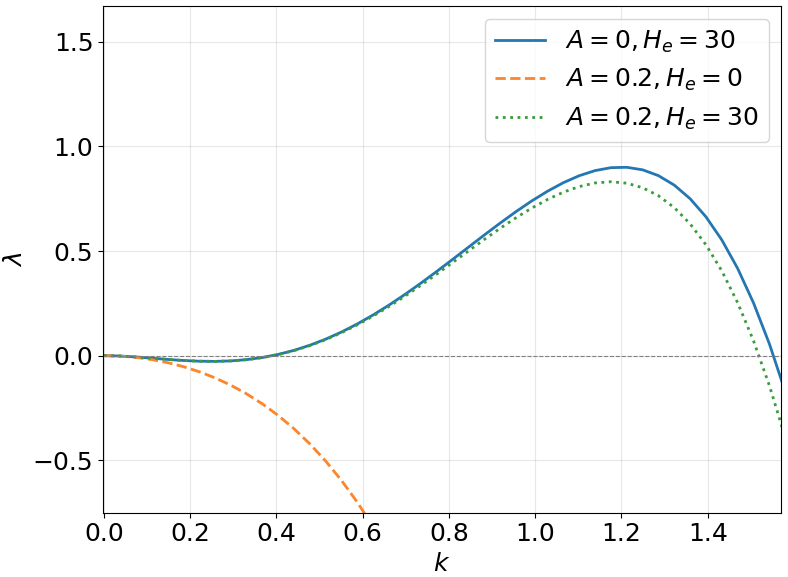
\includegraphics[width=\linewidth]{figures/chap3/A_02.png}
		\caption{}
		\label{fig:A_02}
	\end{subfigure}
	\hfill
	\begin{subfigure}[t]{0.48\textwidth}
		\centering
		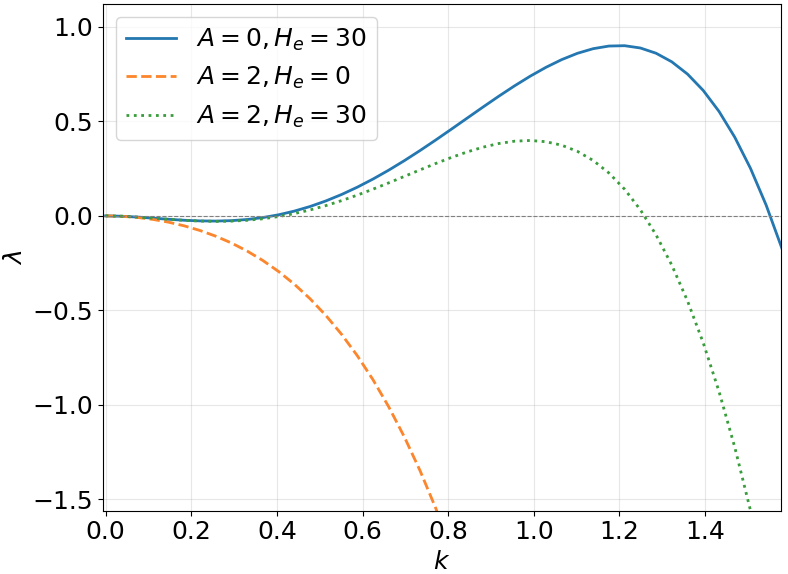
\includegraphics[width=\linewidth]{figures/chap3/A_2.png}
		\caption{}
		\label{fig:A_2}
	\end{subfigure}
	\vspace{0.6cm}
	\begin{subfigure}[t]{0.48\textwidth}
		\centering
		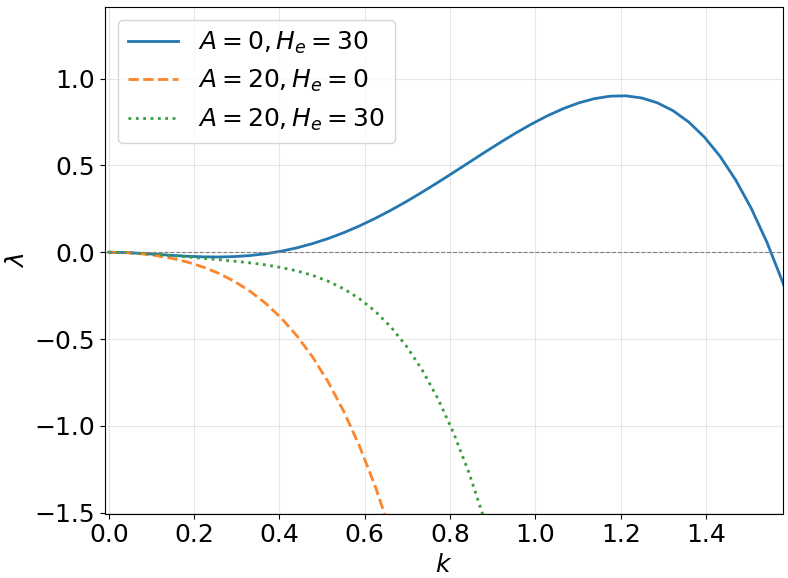
\includegraphics[width=\linewidth]{figures/chap3/A_20.png}
		\caption{}
		\label{fig:A_20}
	\end{subfigure}
	
	\caption{
		Инкремент возмущений как функция волнового числа при разных значениях вибрационного параметра: $A=0.2$ (a), $A=2$ (б), $A=20$ (в). Оранжевая (пунктирная) линия отвечает задаче без магнитного поля, синяя (сплошная) линия -- задача без вибрационного воздействия, зеленая (пунктирная) линия -- рассматриваемая задача. Значения параметров: $\mathrm{G}=3.0, \mathrm{Ca}=3.0, H_{e}=30, \Omega=6.0, \chi=0.5$.
	}
	\label{fig:different_A_ferro}
\end{figure}

Нейтральная кривая устойчивости может быть найдена из условия
\begin{equation}
	\lambda=0
\end{equation}
или, что эквивалентно:
\begin{equation}\label{eq:quadratic_ferro}
	\begin{split}
		 \left( \mathrm{Ca} + \frac{A}{2} (1-m) \right) k^2 - \frac{H_{e}}{(2(1+\chi)+k)} k + \mathrm{G}=0.
	\end{split}
\end{equation}

Длинноволновая неустойчивость (при малых $k$) не зависит от вибраций и поверхностного натяжения, поскольку рост малых возмущений определяется условием
\begin{equation}
	\mathrm{G} - \frac{H_{e}}{(2(1+\chi)+k)} k<0.
\end{equation}

Этот результат согласуется с результатами ранних работ \cite{Korovin2013, Mller1998}. Следует, однако, отметить, что для ограниченного слоя спектр волновых чисел ограничен снизу и является дискретным (при умеренных и больших $k$). Следовательно, в этом случае вклад вибрационной силы и поверхностного натяжения становится более существенным.

Уравнение \eqref{eq:quadratic_ferro} определяет два максимальных значения критического волнового числа $k^{(cr)}$:
\begin{equation}
	\frac{Q_{2}(0)\pm\sqrt{Q_{2}(0)^{2}-4GQ_{1}}}{2Q_{1}},
\end{equation}
где
\begin{equation}
	Q_{1}= \mathrm{Ca}+ \frac{A}{2} (1-m) ,
\end{equation}
\begin{equation}
	Q_{2}(k)=\frac{H_{e}}{2(1+\chi)+k}.
\end{equation}

На рис. \ref{fig:different_A_ferro} приведены графики инкремента возмущений от волнового числа для случая малого, среднего и большого значения вибрационного параметра при $\mathrm{G}=3.0, \mathrm{Ca}=3.0, H_{e}=30, \Omega=6.0, \chi=0.5$.  При малом значении вибрационного параметра  диапазон волновых чисел, при которых система является устойчивой, изменяется слабо (рис. \ref{fig:A_02}). При увеличении интенсивности вибраций диапазон расширяется (рис. \ref{fig:A_2}), а при большой интенсивности вибраций задача устойчива во всем диапазоне волновых чисел (рис. \ref{fig:A_20}). 


\subsection{Выводы по главе}

В данной главе была исследована динамика тонкой пленки магнитной жидкости, бесконечной в продольном направлении, в стационарном вертикальном магнитном поле при воздействии вертикальных вибраций. 

Для анализа использовалось длинноволновое приближение, в рамках которого течение разделялось на пульсационную и осредненную по времени составляющие. 

Показано, что в отсутствие вибраций при малых волновых числах основным механизмом подавления неустойчивости является гравитационная сила, тогда как при больших волновых числах доминирующую роль играют капиллярные силы. Проведенный линейный анализ осредненного течения показал, что вибрационное воздействие приводит к подавлению неустойчивости и, как следствие, к расширению области устойчивости. В частности, вибрации подавляют коротковолновую неустойчивость, оказывая в этом отношении эффект, аналогичный действию поверхностного натяжения. Кроме того, вибрационное воздействие приводит к подавлению и длинноволновой неустойчивости.

Дальнейшее направление исследований данной задачи заключается в получении нелинейного динамического уравнения для свободной границы с учетом вклада магнитного поля, его численное решение и проведение слабонелинейного анализа для уточнения поведения системы вблизи границы развития неустойчивости, а также изучение формирования и эволюции пространственных волновых структур, возникающих в результате нелинейного взаимодействия.


\mychapter{4}{Численное моделирование динамики межфазной границы при вертикальных вибрациях методом решеточных уравнений Больцмана}{chap:LBM}


Данная глава посвящена моделированию задач с динамикой границы раздела при вертикальном вибрационном воздействии методом решеточных уравнений Больцмана. 

Используется схема, основанная на консервативной локальной форме уравнения Аллена--Кана.
Вертикальные вибрации учитываются посредством введения модулированного ускорения свободного падения.

Результаты опубликованы в работе \cite{Volodin2026LBM}. 

\subsection{Макроскопическая постановка задачи}

Для рассматриваемых в данной главе задач макроскопическое описание двухкомпонентной системы несмешивающихся жидкостей со свободно деформируемой границей раздела в изотермической постановке включает уравнения Навье--Стокса, уравнение неразрывности для несжимаемой жидкости и локальное консервативное уравнение Аллена--Кана \cite{Inamuro2021, Sun2007, Liang2018}:
\begin{equation} \label{eq:Navier-Stokes_LBM}
	\rho \left(
	\frac{\partial \mathbf{v}}{\partial t}
	+ (\mathbf{v} \cdot \nabla)\mathbf{v}
	\right)
	=
	- \nabla p
	+ \mu \Delta \mathbf{v}
	+ \mathbf{F_s}
	+ \mathbf{G},
\end{equation}
\begin{equation}
	\nabla \cdot \mathbf{v} = 0,
\end{equation}
\begin{equation}
	\frac{\partial \phi}{\partial t}
	+ \nabla \cdot (\phi \mathbf{v})
	=
	\nabla \cdot
	\left[
	M \left(
	1 - \frac{4\phi\left(1-\phi\right)}{|\nabla \phi| W}
	\right)
	\nabla \phi
	\right],
\end{equation}
где $\mathbf{v}$ -- скорость жидкости, $\phi$ -- параметр порядка,  $M$ -- параметр мобильности, $W$ -- толщина границы раздела, $\rho$ -- плотность жидкости, $p$ -- поле давления, $\mu$ -- динамическая вязкость, $\mathbf{F_s}$ -- сила поверхностного натяжения, $\mathbf{G}=(G_x, G_y)$ -- внешняя объемная сила.

Сила поверхностного натяжения определяется согласно \cite{Geier2015, Liang2018}:
%
\begin{equation}
	\mathbf{F}_{s}
	=
	\left[
	4\beta \phi(\phi - 1)(\phi - \frac{1}{2})
	- \kappa \Delta \phi
	\right]
	\nabla \phi,
\end{equation}
%
где параметры $\beta$ и $\kappa$ связаны с коэффициентом поверхностного натяжения $\alpha$ и толщиной границы раздела $W$ следующим образом:
$$
\beta = \frac{12\alpha}{W},
\qquad
\kappa = \frac{3\alpha W}{2}.
$$

%Слагаемое объемной силы $\mathbf{G} = (G_x, G_y)$ требует специального рассмотрения в контексте рассматриваемых задач. 

В рассматриваемых задачах внешнее воздействие осуществляется исключительно в вертикальном направлении, поэтому $G_x = 0$, а на систему действуют вертикальные гармонические вибрации с частотой $\Omega$ и амплитудой $\mathrm{B}$. Удобно перейти в неинерциальную систему отсчета, связанную с вибрирующим сосудом, введя модулированное ускорение свободного падения:
\begin{equation}\label{eq:vibro_force_LBM}
	G_y = - \rho g + \rho \mathrm{B} \Omega^2 \sin(\Omega t).
\end{equation}

Система уравнений \eqref{eq:Navier-Stokes_LBM}--\eqref{eq:vibro_force_LBM} и граничные условия, которым соответствуют твердые горизонтальные стенки и периодические условия, поставленные на боковые стенки, определяют макроскопическую постановку задачи. 

Отметим, что в рассматриваемых задачах присутствует несколько характерных временных масштабов: акустическое время $t_a \sim L/c_s$, вязкое время $t_{\nu} \sim L^2/\nu$ и вибрационное время $t_{f_v} \sim 2\pi/\Omega$, где $L$ -- характерный размер задачи, $\nu=\mu / \rho$ -- кинематическая вязкость, $c_s$ -- скорость звука. При численном моделировании методом решеточных уравнений Больцмана необходимо выполнение следующих условий \cite{Krger2017}:
$$
t_\nu,\,t_{f_v} \gg t_a.
$$
Кроме того, в данном исследовании рассматривается случай высокочастотных вибраций, в связи с чем дополнительно предполагается выполнение условия:
$$
t_{\nu} \gg t_{f_v}.
$$


\subsection{Метод решеточных уравнений Больцмана для задач с межфазной границей}

Как известно, применимость LBM к гидродинамическим задачам обосновывается тем, что макроскопические уравнения можно получить из кинетической схемы с помощью асимптотического анализа (см., например, \cite{Krger2017, Succi2018, Redeman2014, Viggen2014}). Разложение Чепмена--Энскога \cite{Chapman1991} или Соне \cite{Inamuro2021} показывает, что при малых числах Кнудсена и Маха моменты функций распределения сводятся к уравнениям Навье--Стокса и связанным с ними уравнениям переноса дополнительных полей (температуры, концентрации, параметра порядка и т.п.), вид которых определяется конкретной моделью.

В данной главе рассматривается двумерная постановка, используется приближение с одним временем релаксации (SRT) и решетка D2Q9 (см. рис. \ref{fig:D2Q9_LBM}), в которой весовые коэффициенты в ортогональных направлениях больше, чем в диагональных. 
\begin{figure}[h]
	\centering
	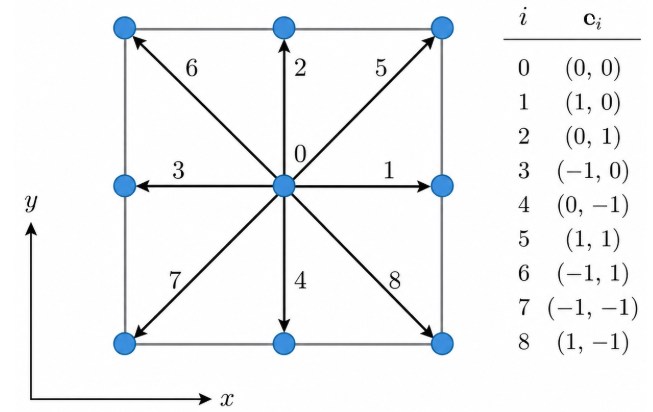
\includegraphics[width=0.47\textwidth]{figures/chap4/D2Q9_.png}
	\caption{Вид решетки D2Q9, $i$ -- номер направления, $\mathbf{c_i}$ -- мезоскопический вектор скорости.}
	\label{fig:D2Q9_LBM}
\end{figure}

Дискретная LBM-схема, использованная в данной работе, приводится в следующем разделе.


\subsubsection{Дискретная схема для восстановления уравнения переноса импульса}

Для восстановления уравнения переноса импульса используется следующая система уравнений \cite{Guo2000, Guo2002, Liang2018}:
\begin{equation}\label{eq:evolution_f_LBM}
		f_i(\mathbf{x}+\mathbf{c}_i \Delta t, t+\Delta t)-f_i(\mathbf{x},t) = -\frac{1}{\tau_f}\left[f_i(\mathbf{x},t)-f_i^{eq}(\mathbf{x},t)\right]  + \Delta t \left(1-\frac{1}{2\tau_f(\mathbf{x},t)}\right) F_i(\mathbf{x},t).
\end{equation}
Равновесная функция распределения имеет вид
\begin{equation}
	f_i^{eq}(\mathbf{x},t)=
	\begin{cases}
		(\omega_0-1)\dfrac{p}{c_s^2} + \rho s_0(\mathbf{v}),
		& i=0,\\
		\omega_i\dfrac{p}{c_s^2} + \rho s_i(\mathbf{v}),
		& i=1,\dots,8.
	\end{cases}
\end{equation}

Здесь $f_i$ и $f_i^{eq}$ являются функциями распределения и равновесными функциями распределения, используемыми для восстановления уравнений Навье--Стокса и неразрывности, $\Delta t$ -- дискретный шаг по времени, $c_s^2=1/3$ -- квадрат скорости звука, $\omega_i$ -- весовые коэффициенты, $\mathbf{c}_i=(c_{ix},c_{iy})$ -- мезоскопический вектор скорости:
$$
	\omega_i =
	\begin{cases}
		\frac{4}{9}, & i=0,\\
		\frac{1}{9}, & i=1,2,3,4,\\
		\frac{1}{36}, & i=5,6,7,8.
	\end{cases}
$$
$$
c_{ix} = \{ 0, 1, 0, -1, 0, 1, -1, -1, 1 \},
$$
$$
c_{iy} = \{ 0, 0, 1, 0, -1, 1, 1, -1, -1 \}.
$$

Величина $\tau_f$ представляет собой время релаксации $f_i$ к локальному равновесию, а функции $s_i(\mathbf{v})$ и $F_i(\mathbf{x},t)$ определяются следующим образом:
\begin{equation}
	s_i(\mathbf{v})=
	\omega_i
	\left[
	\frac{\mathbf{c}_i\cdot\mathbf{v}}{c_s^2}
	+\frac{(\mathbf{c}_i\cdot\mathbf{v})^2}{2c_s^4}
	-\frac{\mathbf{v}\cdot\mathbf{v}}{2c_s^2}
	\right],
\end{equation}
\begin{equation}
	F_i(\mathbf{x},t)=
	\omega_i
	\left[
	\mathbf{v}\cdot\nabla\rho
	+\frac{\mathbf{c}_i\cdot\mathbf{F}}{c_s^2}
	+\frac{\mathbf{v}\cdot\nabla\rho :
		(\mathbf{c}_i\mathbf{c}_i-c_s^2\mathbf{I})}{2c_s^2}
	\right],
\end{equation}
где $\mathbf{I}$ -- единичная матрица, двоеточие обозначает двойную свертку и $\mathbf{F}=\mathbf{F}_s+\mathbf{G}$.

В задачах со свободной границей важными параметрами являются не только отношение плотностей, но и отношение вязкостей двух фаз. Поэтому время релаксации $\tau_f$ должно зависеть от пространственных координат:
\begin{equation*}
	\tau_f(\mathbf{x},t) =
	(\tau_{f_l}-\tau_{f_g})\phi + \tau_{f_g},
\end{equation*}
где $\tau_{f_l}$ и $\tau_{f_g}$ связаны с кинематическими вязкостями тяжелой (индекс $l$) и легкой (индекс $g$) фаз соотношениями
\begin{equation*}
	\tau_{f_l}=
	\frac{\nu_l}{c_s^2 \Delta t}+\frac{1}{2},
	\qquad
	\tau_{f_g}=
	\frac{\nu_g}{c_s^2 \Delta t}+\frac{1}{2}.
\end{equation*}

Макроскопические переменные определяются через функции распределения следующим образом:
\begin{equation}
	\rho\mathbf{v}=\sum_{i=0}^{8} f_i \mathbf{c}_i + \frac{1}{2}\Delta t\,\mathbf{F},
\end{equation}
\begin{equation}
	p=\frac{c_s^2}{1-\omega_0}
	\left[
	\sum_{i=1}^{8} f_i
	+\frac{\Delta t}{2}(\rho_l-\rho_g)\,\mathbf{v}\cdot\nabla\phi
	+\rho s_0(\mathbf{v})
	\right].
\end{equation}


В LBM градиенты любой скалярной величины $\zeta$ могут быть вычислены с использованием стандартных дискретных соотношений \cite{Ren2016, Liu2014, Liang2018}:

$$
\nabla \zeta(\mathbf{x})=
\frac{1}{\Delta t\,c_s^2}
\sum_{i=1}^{8}
\omega_i \mathbf{c}_i
\zeta(\mathbf{x}+\mathbf{c}_i\Delta t),
$$

$$
\Delta \zeta(\mathbf{x})=
\frac{1}{\Delta t^2 c_s^2}
\sum_{i=1}^{8}
2\omega_i
\left[
\zeta(\mathbf{x}+\mathbf{c}_i\Delta t)-\zeta(\mathbf{x})
\right].
$$
	
\subsubsection{Дискретная схема для восстановления уравнения для параметра порядка}
	
Для описания консервативного локального уравнения Аллена--Кана используется следующая система уравнений \cite{Geier2015, Liang2018}:
\begin{equation}
	\begin{split}
		g_i(\mathbf{x}+\mathbf{c}_i \Delta t, t+\Delta t)
		-g_i(\mathbf{x},t)
		&=
		-\frac{1}{\tau_g}
		\left[
		g_i(\mathbf{x},t)-g_i^{eq}(\mathbf{x},t)
		\right] \\
		&\quad+
		\Delta t
		\left(
		1-\frac{1}{2\tau_g}
		\right)
		R_i(\mathbf{x},t),
	\end{split}
\end{equation}
\begin{equation}
	g_i^{eq}(\mathbf{x},t)=
	\omega_i \phi
	\left(
	1+\frac{\mathbf{c}_i\cdot\mathbf{v}}{c_s^2}
	\right).
\end{equation}
Здесь $g_i$ и $g_i^{eq}$ являются соответственно функцией распределения и равновесной функцией распределения, используемыми для определения эволюции параметра порядка,
$$
\tau_g=
\frac{M}{c_s^2 \Delta t}+\frac{1}{2}
$$
есть время релаксации $g_i$ к локальному равновесию, а $\omega_i$ --- весовые коэффициенты.
Слагаемое $R_i$ определяется выражением:
\begin{equation}
	R_i(\mathbf{x},t)=
	\frac{\omega_i}{c_s^2}
	\mathbf{c}_i\cdot
	\left[
	\frac{\partial(\phi \mathbf{v})}{\partial t}
	+
	c_s^2
	\frac{\nabla \phi}{|\nabla \phi|}
	\frac{4\phi(1-\phi)}{W}
	\right].
\end{equation}

Параметр порядка определяется суммированием по всем направлениям:
\begin{equation}
	\phi=\sum_{i=0}^{8} g_i.
\end{equation}
Плотность выражается через параметр порядка следующим образом:
\begin{equation}\label{eq:rho_through_phi_LBM}
	\rho=(\rho_l-\rho_g)\phi+\rho_g.
\end{equation}

Дискретная схема \eqref{eq:evolution_f_LBM}--\eqref{eq:rho_through_phi_LBM} в макроскопическом пределе воспроизводит уравнения Навье--Стокса, уравнение неразрывности для несжимаемой жидкости и локальное уравнение Аллена--Кана \cite{Wang2016, Liang2018}, записанные с учетом воздействия вертикальных вибраций (см. \eqref{eq:vibro_force_LBM}) в неинерциальной системе отсчета.

В работе использовались граничные условия типа wet-node, толщина границы раздела задавалась равной $W=5$, плотность легкой фазы принималась равной $\rho_g=1.0$, а время релаксации, связанное с параметром мобильности, задавалось равным $\tau_g=1.0$. В дальнейшем значения параметров будут приводиться в безразмерных единицах.

Приведенный выше алгоритм был реализован на языке C++. 
%Все вычисления выполнялись на процессоре с архитектурой ARM без использования параллелизации. Визуализация и постобработка результатов проводились с использованием библиотеки Matplotlib.


%Полученные в настоящей работе численные результаты представлены преимущественно в виде цветовых карт поля плотности, где желтый цвет соответствует тяжелой фазе, а синий --- легкой фазе. Анализ результатов носит преимущественно качественный характер, при этом для каждого режима указываются соответствующие безразмерные параметры, обеспечивающие его корректную физическую характеристику.

\subsection{Верификация численной схемы}

Одной из классических задач, используемых для проверки разрешения межфазной границы в численных методах, является неустойчивость Рэлея--Тейлора -- гравитационная неустойчивость границы раздела двух жидкостей, при которой более плотная жидкость первоначально располагается над менее плотной.

\subsubsection{Сравнение с линейной теорией устойчивости}

Проведем сравнение численных результатов с линейной теорией неустойчивости Рэлея--Тейлора. Хорошо известно, что на ранней стадии развития неустойчивости, когда амплитуда возмущения мала по сравнению с длиной волны, амплитуда возмущения изменяется по закону
%
\begin{equation*}
	h = h_0 \exp(\gamma t),
\end{equation*}
%
где $h_0$ -- начальная амплитуда возмущения, а $\gamma$ -- скорость роста возмущения. Аналитическая оценка скорости роста имеет вид~\cite{Chandrasekhar1981}:
\begin{equation*}
	\gamma^2 = kg\left(\frac{\rho_l - \rho_g}{\rho_l + \rho_g}
	- \frac{\alpha k^2}{g\left(\rho_l + \rho_g\right)}\right),
\end{equation*}
где $k = 2\pi/L$, а $L$ в данном случае является длиной волны начального возмущения.

Для сравнения численных результатов с аналитическим решением на ранней стадии развития неустойчивости и определения скорости роста начальное возмущение межфазной границы задавалось в виде
%
\begin{equation*}
	y_{\mathrm{interface}} = \frac{N_y}{2}
	+ 0.01\,N_y \cos\!\left(\frac{2\pi x}{N_x}\right),
\end{equation*}
%
где $N_x$ и $N_y$ --- число узлов сетки в направлениях $x$ и $y$ соответственно, при этом начальное поле скорости полагалось равным нулю. Скорость роста возмущения в численных экспериментах определялась по скорости опускания тяжелой жидкой фазы в центре расчетной области, $x = N_x/2$. Волновое число $k$ изменялось путем изменения значения $N_x$.

Параметры численных экспериментов имели следующие значения:
$\rho_l = 3$, $\rho_g = 1$, $\alpha = 0.01$, $g = 1.5\cdot10^{-5}$,
$\nu_l/\nu_g = 1.0$.

Результаты аналитической оценки и численного моделирования представлены на рис.~\ref{fig:RT-growth-rate_LBM}. Наблюдается очень хорошее согласие между численными результатами и аналитическим предсказанием.

\begin{figure}[h]
	\centering
	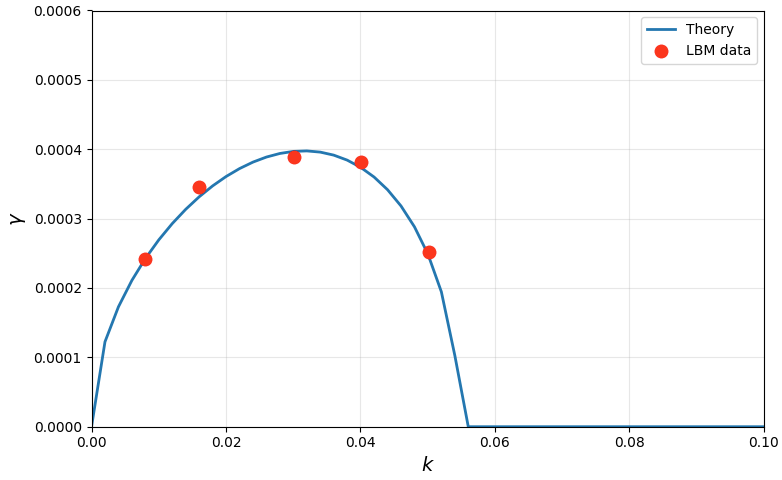
\includegraphics[width=0.77\textwidth]{figures/chap4/RT/RT_linear_comparison.png}
	\caption{Сравнение численно полученной скорости роста $\gamma$ с аналитическим предсказанием в зависимости от волнового числа $k$.}
	\label{fig:RT-growth-rate_LBM}
\end{figure}

% -----------------------------------------------------------------------
\subsubsection{Исследование сеточной зависимости}
% -----------------------------------------------------------------------

Для исследования сеточной зависимости использовалась задача Рэлея--Тейлора при фиксированном числе Бонда и различных размерах расчетной области. Анализ проводился для размеров области
$50\times100$, $100\times200$, $200\times400$, $300\times600$, $400\times800$
и $500\times1000$ узлов. Параметры моделирования фиксировались:
$\nu_r = \nu_l/\nu_g = 1$, $\rho_r = \rho_l/\rho_g = 3$, $\mathrm{Bo} = 200$, где число Бонда определяется следующим образом:
\begin{equation}
	\mathrm{Bo} = \frac{(\rho_l - \rho_g)\,g L^2}{\alpha},
\end{equation}
что представляет собой удобную безразмерную характеристику данной неустойчивости и определяет отношение гравитационной силы к силе поверхностного натяжения.

В качестве количественной меры относительной численной погрешности использовалась усредненная по времени амплитуда проникновения $\gamma_n$ тяжелой жидкой фазы в центре области ($x = N_x/2$). Соответствующие результаты представлены в табл.~\ref{tab:RT-grid_LBM}. 

\begin{table}
	\centering
	\caption{Результаты исследования сеточной зависимости.}
	\label{tab:RT-grid_LBM}
	\begin{tabular}{lccc}
		\hline
		Размер сетки & $\gamma_n$ & Погрешность & Время CPU \\
		\hline
		$50\times100$   & $8.082\cdot10^{-5}$  & $54.55\%$ & $1/6$ \\
		$100\times200$  & $1.348\cdot10^{-4}$  & $24.19\%$  & $1/3$ \\
		$200\times400$  & $1.702\cdot10^{-4}$  & $4.28\%$   & $1$ \\
		$300\times600$  & $1.759\cdot10^{-4}$  & $1.07\%$   & $2.5$ \\
		$400\times800$  & $1.770\cdot10^{-4}$  & $0.45\%$  & $4.5$ \\
		$500\times1000$ & $1.778\cdot10^{-4}$  & ---       & $6.5$ \\
		\hline
	\end{tabular}
\end{table}

Исходя из баланса между вычислительными затратами и оцененной относительной погрешностью, в качестве базового было выбрано разрешение расчетной области $200\times400$ узлов. При последующих расчетах размеры сетки корректировались с учетом геометрии задачи, сохраняя при этом аналогичное пространственное разрешение.

\subsubsection{Неустойчивость Рэлея--Тейлора}

Для бесконечно протяженной межфазной границы неустойчивость развивается при любых значениях параметров. Известно (см., например,~\cite{Chandrasekhar1981, Sharp1984}), что конечный размер расчетной области приводит к появлению критической длины волны и неустойчивость может развиваться только в том случае, если эта длина волны меньше характерного размера расчетной области. Следовательно, можно выбрать параметры таким образом, чтобы критическая длина волны превышала размер расчетной области, полностью подавляя тем самым развитие неустойчивости.

Критическое волновое число, разделяющее растущие и затухающие возмущения, определяется соотношением~\cite{Briskman1976, Bezdenezhnykh1982, Bezdenezhnykh1983}: $k_* = \sqrt {\rho_l g/\alpha}.$
При $k = 2\pi/L > k_*$, где $L$ является продольным размером расчетной области, возмущения затухают и неустойчивость не развивается, при $k = 2\pi/L < k_*$ возмущения растут, и первоначально неустойчивое расположение жидкостей в конечном итоге разрушается.

В данном разделе рассматриваются два режима: $\mathrm{Bo} = 10$ и $\mathrm{Bo} = 200$.
Для $\mathrm{Bo} = 10$ выполняется условие $k > k_*$, поэтому межфазная граница является устойчивой и развития неустойчивости не ожидается. Напротив, для $\mathrm{Bo} = 200$ выполняется условие $k < k_*$, что соответствует неустойчивому режиму.

\begin{figure} 
	\centering
	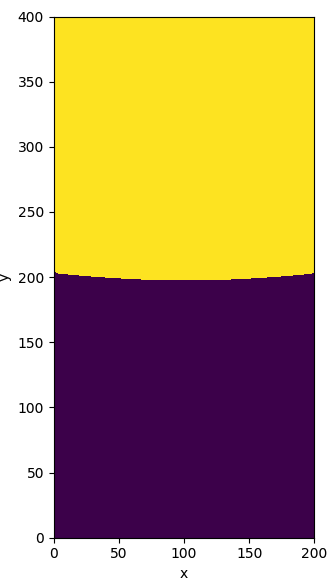
\includegraphics[width=0.35\textwidth]{figures/chap4/RT/RT_Bo10.png}
	\caption{Стационарное состояние поля плотности при $\mathrm{Bo}=10$. Желтым цветом показана тяжелая фаза, синим --- легкая фаза.}
	\label{fig:rtbo10_LBM}
\end{figure}

\begin{figure*}
	\centering
	
	\begin{minipage}{0.33\textwidth}
		\centering
		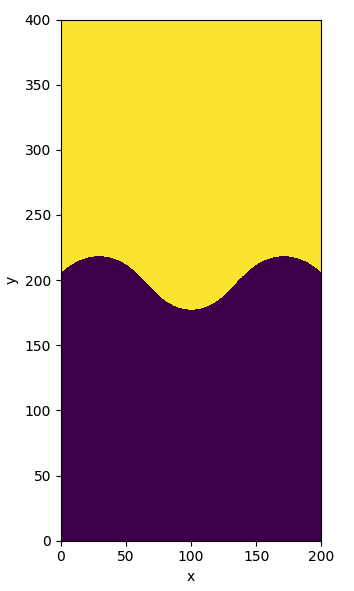
\includegraphics[width=\textwidth]{figures/chap4/RT/rho_25000_Bo200.png}\\
		(a)
	\end{minipage}
	\hspace{0.03\textwidth}
	\begin{minipage}{0.33\textwidth}
		\centering
		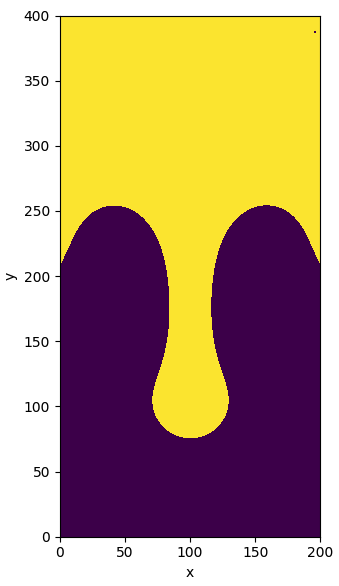
\includegraphics[width=\textwidth]{figures/chap4/RT/rho_35000_Bo200.png}\\
		(b)
	\end{minipage}
	
	\vspace{0.5cm}
	
	\begin{minipage}{0.33\textwidth}
		\centering
		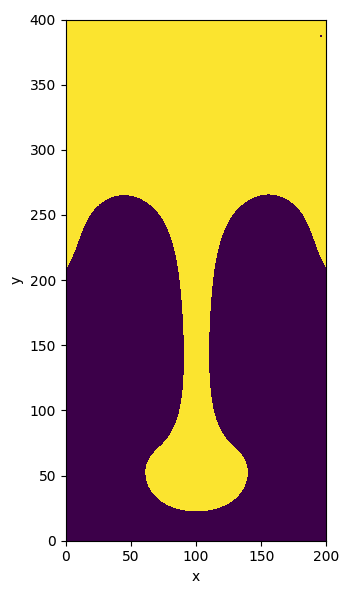
\includegraphics[width=\textwidth]{figures/chap4/RT/rho_38000_Bo200.png}\\
		(c)
	\end{minipage}
	\hspace{0.03\textwidth}
	\begin{minipage}{0.33\textwidth}
		\centering
		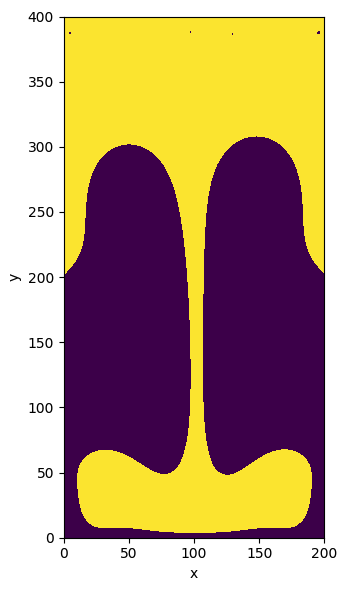
\includegraphics[width=\textwidth]{figures/chap4/RT/rho_50000_Bo200.png}\\
		(d)
	\end{minipage}
	
	\caption{Развитие неустойчивости Рэлея--Тейлора при $\mathrm{Bo}=200$, $\mathrm{We}=0$ на различных временных шагах: $t=25 \cdot 10^3$ (a), $t=35 \cdot 10^3$ (b), $t=38 \cdot 10^3$ (c), $t=50 \cdot 10^3$ (d).}
	\label{fig:RT-development_LBM}
\end{figure*}

Оба случая моделировались на сетке $200 \times 400$ с условиями прилипания на всех границах расчетной области. Начальное условие соответствовало нулевой скорости во всей расчетной области и плоской межфазной границе, расположенной при $y = N_y/2$, при этом
$\rho_r = \rho_l/\rho_g = 6$, $g = 10^{-5}$, $\nu_r = \nu_l/\nu_g = 1$.
Как видно из полей плотности, представленных на рис.~\ref{fig:rtbo10_LBM}--\ref{fig:RT-development_LBM}, при $\mathrm{Bo} = 10$ межфазная граница остается устойчивой и неустойчивость не развивается, тогда как увеличение числа Бонда до $\mathrm{Bo} = 200$ приводит к выраженной деформации межфазной границы. Временная эволюция неустойчивости на выбранных временных шагах расчета представлена на рис.~\ref{fig:RT-development_LBM}.

\subsubsection{Влияние вибраций на неустойчивость Рэлея--Тейлора}

Ранее было показано (см., например, \cite{Piriz2010, Meerkov1984, Briskman1976, Bezdenezhnykh1982, Bezdenezhnykh1983}), что вертикальное вибрационное воздействие может динамически стабилизировать отдельные моды неустойчивости Рэлея--Тейлора и при соответствующих условиях стабилизировать систему в целом. 

В данном подразделе будет показано, что разработанный алгоритм позволяет моделировать изменение основной моды неустойчивости из-за действия вертикальных вибраций.

Для характеристики вибрационного воздействия введем число Вебера, представляющее собой отношение вибрационной силы к силе поверхностного натяжения:
\begin{equation}
	\mathrm{We} = \frac{(\rho_l - \rho_g) (\mathrm{B} \Omega)^2 L}{\alpha}.
\end{equation}

\begin{figure*}
	\centering
	\begin{minipage}{0.33\textwidth}
		\centering
		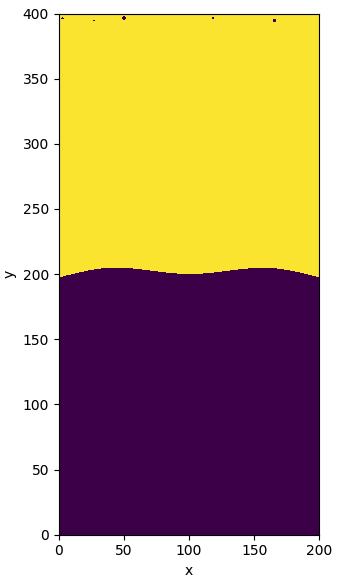
\includegraphics[width=\textwidth]{figures/chap4/RT/rho_25000_Bo200_vibr.png}\\
		(a)
	\end{minipage}
	\hspace{0.015\textwidth}
	\begin{minipage}{0.33\textwidth}
		\centering
		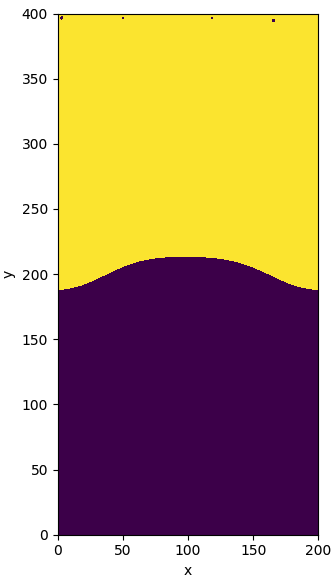
\includegraphics[width=\textwidth]{figures/chap4/RT/rho_35000_Bo200_vibr.png}\\
		(б)
	\end{minipage}
	\hspace{0.015\textwidth}
	\begin{minipage}{0.33\textwidth}
		\centering
		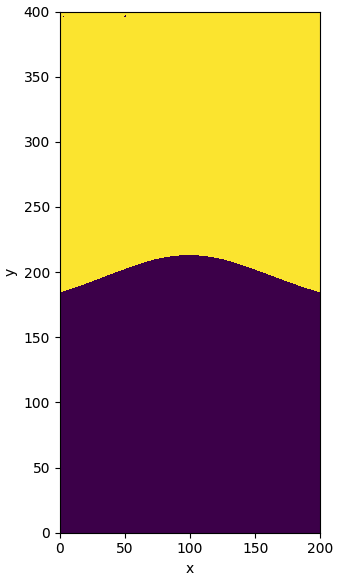
\includegraphics[width=\textwidth]{figures/chap4/RT/rho_38000_Bo200_vibr.png}\\
		(в)
	\end{minipage}
	\hspace{0.015\textwidth}
	\begin{minipage}{0.33\textwidth}
		\centering
		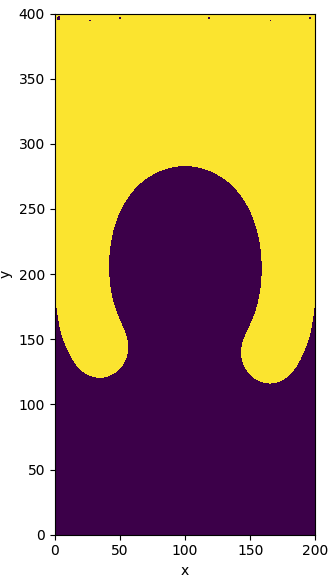
\includegraphics[width=\textwidth]{figures/chap4/RT/rho_50000_Bo200_vibr.png}\\
		(г)
	\end{minipage}
	
	\caption{Изменение основной моды неустойчивости Рэлея--Тейлора при $\mathrm{Bo}=200$, $\mathrm{We}=90$ на различных временных шагах: $t=25 \cdot 10^3$ (a), $t=35 \cdot 10^3$ (б), $t=38 \cdot 10^3$ (в), $t=50 \cdot 10^3$ (г).}
	\label{fig:RT-suppression_LBM}
\end{figure*}


Как показано на рис.~\ref{fig:RT-suppression_LBM}, вертикальное вибрационное воздействие при \(\mathrm{Bo} = 200\) и \(\mathrm{We} = 90\) (\(\Omega = 6 \cdot 10^{-4}\), $\mathrm{B}=50$) изменяет основную моду неустойчивости, которая соответствует продольному размеру расчетной области.

Таким образом, в данной численной реализации введение вибрационного воздействия с частотой $\Omega = 6 \cdot 10^{-4}$ с точки зрения критической длины волны приводит к уменьшению характерного размера области в два раза.


\subsection{Возникновение гравитационно-капиллярных волн под действием вертикальных вибраций}

Вертикальное вибрационное воздействие может приводить к движению межфазной границы в двухслойной системе. Рассмотрим возникновение гравитационно-капиллярных волн, вызванное внешним вибрационным воздействием, при $g=10^{-5}$, $\alpha=5 \cdot 10^{-2}$, $\nu_r=1$, $\rho_r=6.0$, $\mathrm{Bo}=160$ и различных значениях $\Omega$ и $\mathrm{B}$. В начальный момент тяжелая жидкость находилась в нижней половине расчетной области, а межфазная граница представляла собой невозмущенную горизонтальную поверхность, расположенную на уровне $y=N_y/2$. Начальное поле скорости полагалось нулевым.

\begin{figure*}
	\centering
	\begin{minipage}{0.4\textwidth}
		\centering
		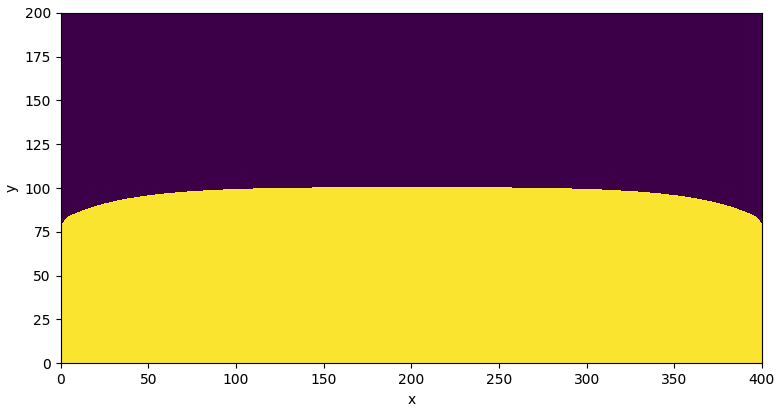
\includegraphics[width=\textwidth]{figures/chap4/waves/weak/init.png}
		\
		(a)
	\end{minipage}
	\vspace{0.5em}
	\begin{minipage}{0.4\textwidth}
		\centering
		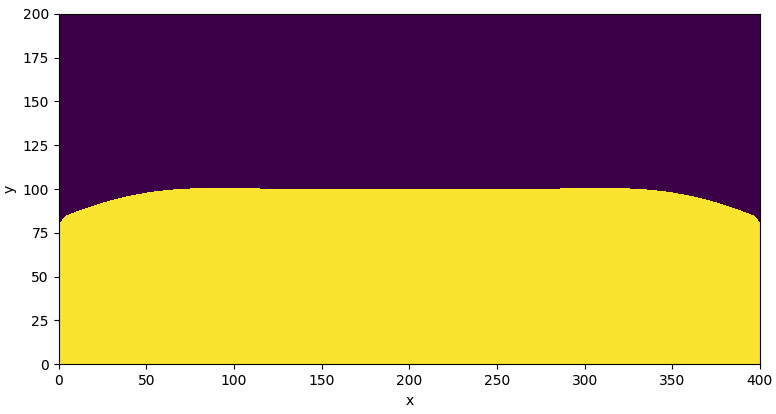
\includegraphics[width=\textwidth]{figures/chap4/waves/weak/127.png}
		\
		(б)
	\end{minipage}
	\vspace{0.5em}
	\begin{minipage}{0.4\textwidth}
		\centering
		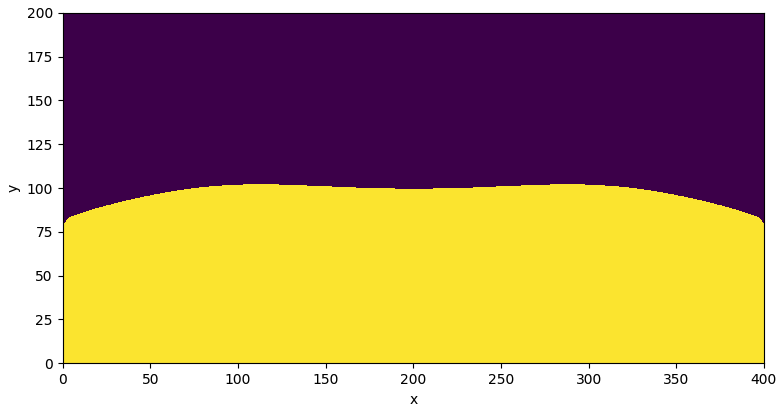
\includegraphics[width=\textwidth]{figures/chap4/waves/weak/129.png}
		\
		(в)
	\end{minipage}
	\vspace{0.5em}
	\begin{minipage}{0.4\textwidth}
		\centering
		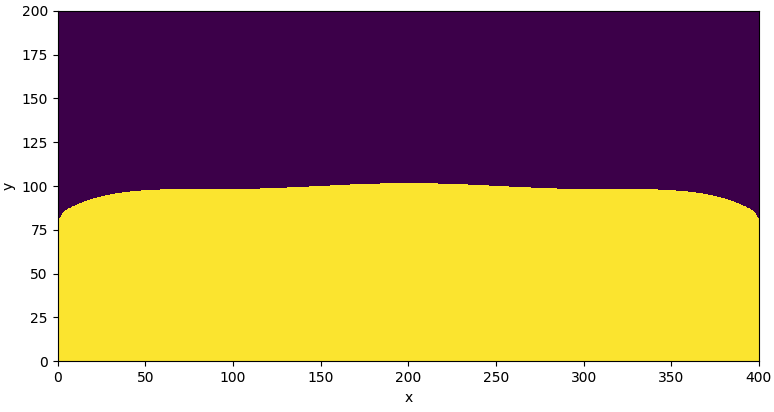
\includegraphics[width=\textwidth]{figures/chap4/waves/weak/133.png}
		\
		(г)
	\end{minipage}
	\caption{Гравитационно-капиллярные волны при $\mathrm{Bo}=160$,
		$\mathrm{We}\approx14$ на различных временных шагах:
		стационарное состояние в отсутствие вибрации (a),
		$t=127\cdot10^3$ (б), $t=129\cdot10^3$ (в),
		$t=133\cdot10^3$ (г).}
	\label{fig:gravity_waves1_LBM}
\end{figure*}

%Было проведено три численных эксперимента. Во всех расчетах начальное условие соответствовало плоской невозмущенной межфазной границе, расположенной при $y=N_y/2$.

Для определения равновесной формы межфазной границы в гравитационном поле моделировалась эволюция системы в отсутствие вибрационного воздействия. Межфазная граница несколько отклоняется от плоской недеформированной, как показано на рис.~\ref{fig:gravity_waves1_LBM}(a). Данная деформация обусловлена действием поверхностных сил, стремящихся придать более тяжелой жидкости форму, близкую к сферической.

\begin{figure}
	\centering
	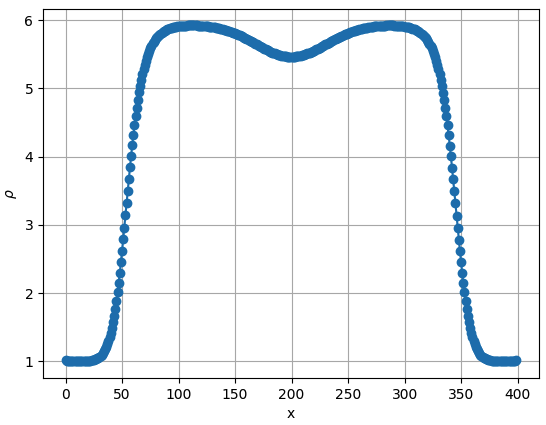
\includegraphics[width=0.65\textwidth]{figures/chap4/waves/weak/rho_98.png}
	\caption{Продольное сечение поля плотности при $t=129 \cdot 10^3$ для $y=98$ при слабых гравитационно-капиллярных волнах ($\mathrm{Bo}=160$, $\mathrm{We}\approx14$).}
	\label{fig:rho_98_LBM}
\end{figure}

Рассмотрим случай относительно слабого вибрационного воздействия при $\Omega \approx 75.6 \cdot 10^{-5}$ и $\mathrm{B}=25$ ($\mathrm{We}\approx14$). На рис.~\ref{fig:gravity_waves1_LBM}(b)--\ref{fig:gravity_waves1_LBM}(d) приведены мгновенные распределения поля плотности, полученные приблизительно за один период колебаний. Продольное сечение поля плотности при $t=129 \cdot 10^3$ для $y=98$ представлено на рис.~\ref{fig:rho_98_LBM}. 

Оценим характерную длину волны из дисперсионного соотношения для гравитационно-капиллярных волн \cite{Landau1986}:
\begin{equation}
	\Omega^2 = k g + \frac{\alpha}{\rho} k^3,
	\label{eq:Landau_LBM}
\end{equation}
где $\Omega$ это частота бегущей волны и собственная частота колебательной моды межфазной границы для волнового числа $k$.
Таким образом, можно сопоставить частоту вынужденных колебаний поверхности с частотой, получаемой из данного дисперсионного соотношения. Из уравнения~(\ref{eq:Landau_LBM}) получаем
\[
L = \frac{2\pi}{k} \approx 200,
\]
что находится в количественном соответствии с результатами численного эксперимента.

Удвоение амплитуды вибрационного воздействия и соответствующее увеличение числа Вебера до $\mathrm{We}\approx57.25$ приводит к режиму, при котором амплитуда волны уже не укладывается в расчетную область. Поэтому в данном случае говорить о распространяющейся вдоль межфазной границы бегущей волне некорректно. Вместо этого наблюдается эффект, который можно интерпретировать как эффективное <<всплытие>> тяжелой жидкости. Данный эффект будет рассмотрен в следующем разделе.

\begin{figure*}
	\centering
	\begin{minipage}{0.4\textwidth}
	
	\centering
	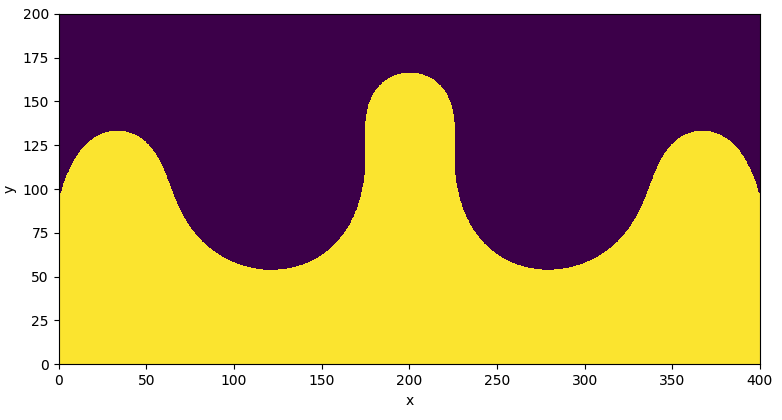
\includegraphics[width=\textwidth]{figures/chap4/waves/strong/181000.png}\
	(a)
	\end{minipage}
	\vspace{0.5em}
	\begin{minipage}{0.4\textwidth}
	\centering
	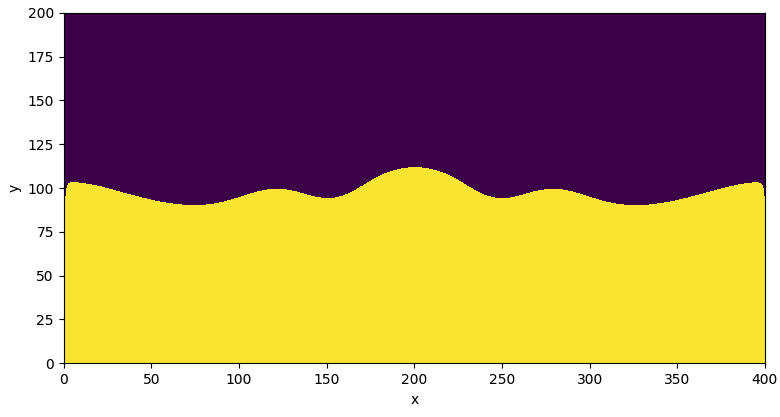
\includegraphics[width=\textwidth]{figures/chap4/waves/strong/183000.png}\
	(б)
	\end{minipage}
	\vspace{0.5em}
	\begin{minipage}{0.4\textwidth}
	\centering
	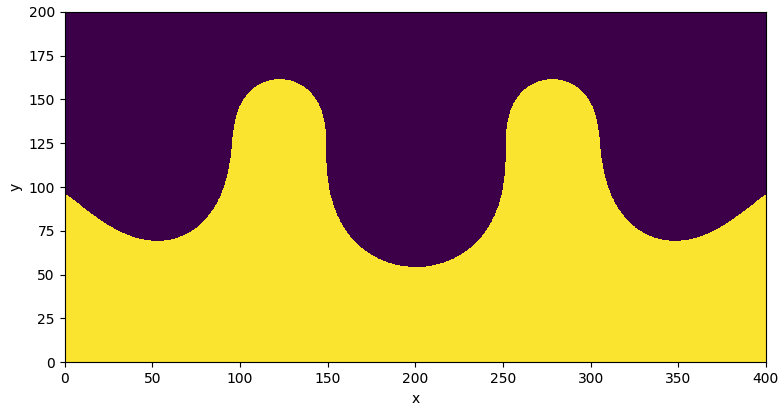
\includegraphics[width=\textwidth]{figures/chap4/waves/strong/185000.png}\
	(в)
	\end{minipage}
	\vspace{0.5em}
	\begin{minipage}{0.4\textwidth}
	\centering
	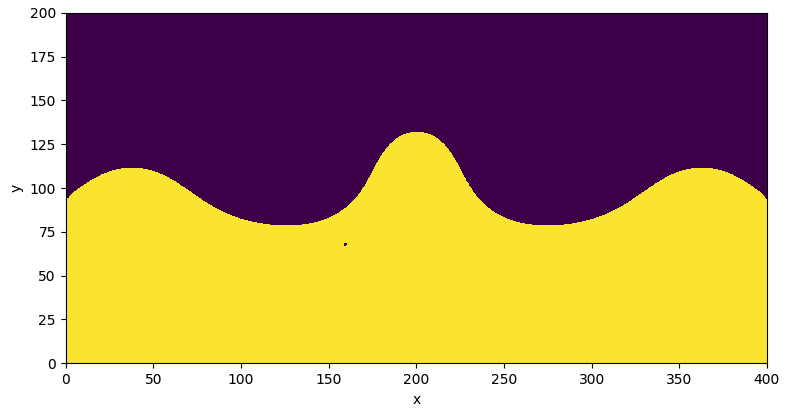
\includegraphics[width=\textwidth]{figures/chap4/waves/strong/188000.png}\
	(г)
	\end{minipage}
	\caption{Гравитационно-капиллярные волны при $\mathrm{Bo}=160$,
	$\mathrm{We}\approx57$ на различных временных шагах:
	$t=181\cdot10^3$ (a), $t=183\cdot10^3$ (б),
	$t=185\cdot10^3$ (в), $t=188\cdot10^3$ (г).}
	\label{fig:gravity_waves2_LBM}
\end{figure*}

\begin{figure}
	\centering
	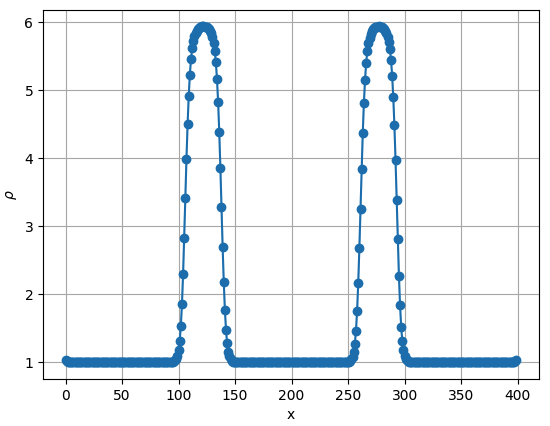
\includegraphics[width=0.65\textwidth]{figures/chap4/waves/strong/rho_157.png}
	\caption{Продольное сечение поля плотности при $t=185 \cdot 10^3$ для $y=155$ при гравитационно-капиллярных волнах с относительно большой амплитудой ($\mathrm{Bo}=160$, $\mathrm{We}\approx57$).}
	\label{fig:rho_157_LBM}
\end{figure}

Число Вебера $\mathrm{We}\approx57$ также может быть достигнуто путем удвоения частоты вибрации: $\Omega\approx15.1 \cdot 10^{-4}$. Результаты данного численного эксперимента представлены на рис.~\ref{fig:gravity_waves2_LBM}. Увеличение частоты вибрационного воздействия приводит к соответствующему уменьшению характерной длины волны гравитационно-капиллярной волны (см. рис.~\ref{fig:rho_157_LBM}).


\subsection{Движение слоя жидкости под действием вертикальных вибраций}

В данном разделе рассмотрено движение слоя под действием вертикальных вибраций. Сосуд с твердыми стенками заполнен двухфазной системой, состоящей из двух несмешивающихся жидкостей, причем более тяжелая фаза первоначально располагается в нижней части расчетной области. Результаты численного моделирования показывают, что под действием вертикальных вибраций можно индуцировать подъем тяжелой фазы к верхней границе расчетной области. В начальный момент тяжелая фаза занимает область $0 \le y \le N_y/5$, а поле скорости во всей расчетной области принимается равным нулю.

Удобно ввести параметр:
\begin{equation}
\Gamma = \frac{\mathrm{B} \Omega^2}{g},
\end{equation}
который характеризует отношение вибрационного ускорения к ускорению свободного падения.

Задачи решались на расчетной сетке $200 \times 500$ при следующих параметрах:
$$
\begin{aligned}
	\rho_r = 100, \qquad \nu_r \approx \frac{1}{3},\qquad \mathrm{Bo} \approx 80, \qquad \Omega \approx 3.17 \cdot 10^{-5}.
\end{aligned}
$$
При этом амплитуда вибраций, а следовательно, параметры $\Gamma$ и $\mathrm{We}$, варьировались.



Мгновенные распределения плотности при $\mathrm{We} \approx 6.3 \cdot 10^{5}$ и $\Gamma = 40$ представлены на рис.~\ref{fig:rise_series_LBM}. Как показано на рис.~\ref{fig:rise_series_LBM}a, под действием вибраций жидкость поднимается к верхней стенке сосуда и достигает ее на рис.~\ref{fig:rise_series_LBM}б--\ref{fig:rise_series_LBM}в. Затем жидкость начинает стекать обратно в нижнюю часть сосуда (рис.~\ref{fig:rise_series_LBM}г--\ref{fig:rise_series_LBM}д), после чего движение вверх возобновляется (рис.~\ref{fig:rise_series_LBM}е). Таким образом, движение носит периодический характер.



\begin{figure*}
	\centering
	% ---- первый ряд ----
	\begin{subfigure}{0.23\textwidth}
		\centering
		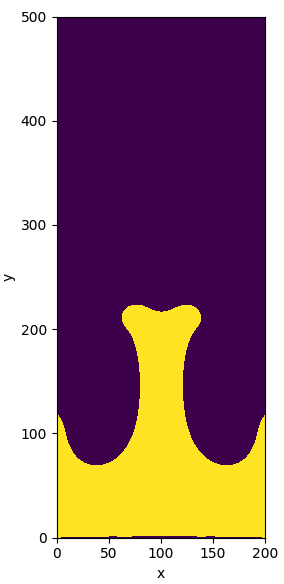
\includegraphics[width=\linewidth]{figures/chap4/rise/10.png}
		\caption{$t=10 \cdot 10^3$}
	\end{subfigure}
	\hfill
	\begin{subfigure}{0.23\textwidth}
		\centering
		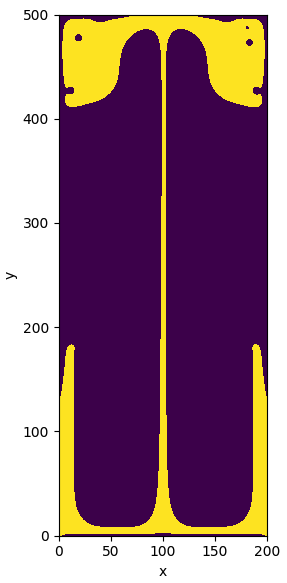
\includegraphics[width=\linewidth]{figures/chap4/rise/17.png}
		\caption{$t=17 \cdot 10^3$}
	\end{subfigure}
	\hfill
	\begin{subfigure}{0.23\textwidth}
		\centering
		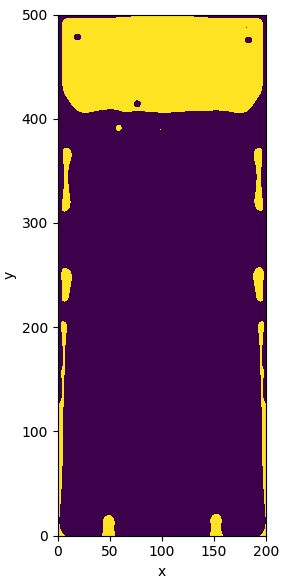
\includegraphics[width=\linewidth]{figures/chap4/rise/50.png}
		\caption{$t=50 \cdot 10^3$}
	\end{subfigure}
	\hfill
	\begin{subfigure}{0.23\textwidth}
		\centering
		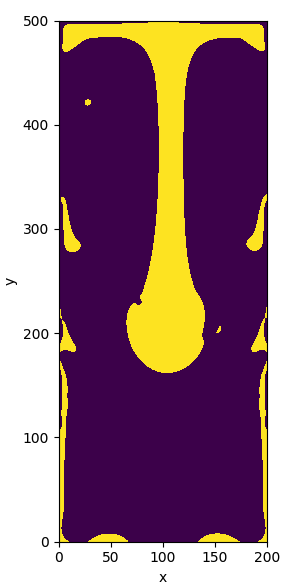
\includegraphics[width=\linewidth]{figures/chap4/rise/65.png}
		\caption{$t=65 \cdot 10^3$}
	\end{subfigure}
	
	\vspace{0.4cm}
	
	% ---- второй ряд ----
	\begin{subfigure}{0.23\textwidth}
		\centering
		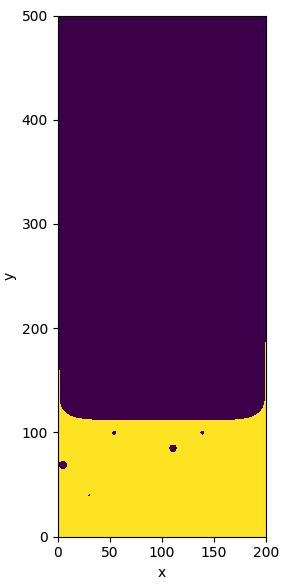
\includegraphics[width=\linewidth]{figures/chap4/rise/150.png}
		\caption{$t=150 \cdot 10^3$}
	\end{subfigure}
	\hfill
	\begin{subfigure}{0.23\textwidth}
		\centering
		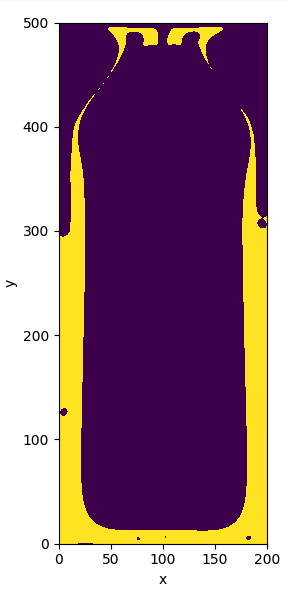
\includegraphics[width=\linewidth]{figures/chap4/rise/172.png}
		\caption{$t=172 \cdot 10^3$}
	\end{subfigure}
	\hfill
	\begin{subfigure}{0.23\textwidth}
		\centering
		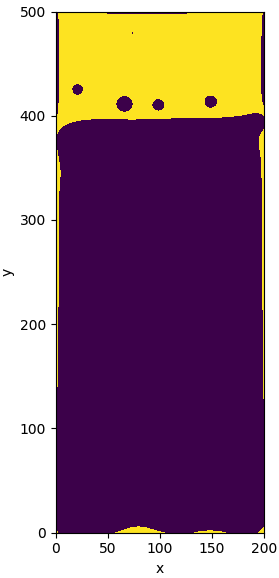
\includegraphics[width=\linewidth]{figures/chap4/rise/250.png}
		\caption{$t=250 \cdot 10^3$}
	\end{subfigure}
	\hfill
	\begin{subfigure}{0.23\textwidth}
		\centering
		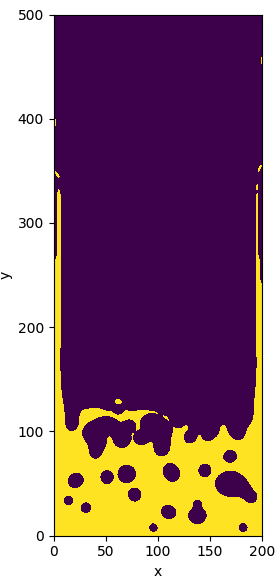
\includegraphics[width=\linewidth]{figures/chap4/rise/500.png}
		\caption{$t=500 \cdot 10^3$}
	\end{subfigure}
	
	\caption{Динамика подъема в различные моменты времени при $\mathrm{Bo}=80$, $\mathrm{We}\approx 6.3 \cdot 10^5$, $\Gamma=40$.}
	\label{fig:rise_series_LBM}	
\end{figure*}

\begin{figure*}
	\centering
	% ---- первый ряд ----
	\begin{subfigure}{0.23\textwidth}
		\centering
		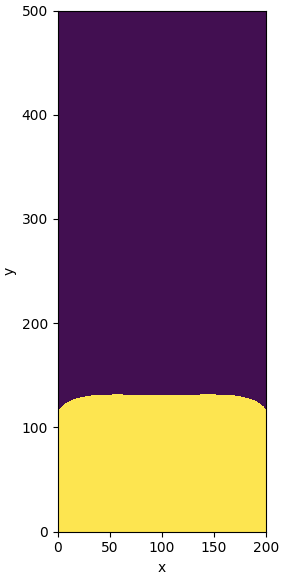
\includegraphics[width=\linewidth]{figures/chap4/rise/series2/500.png}
		\caption{$t=500 \cdot 10^3$}
	\end{subfigure}
	\hfill
	\begin{subfigure}{0.23\textwidth}
		\centering
		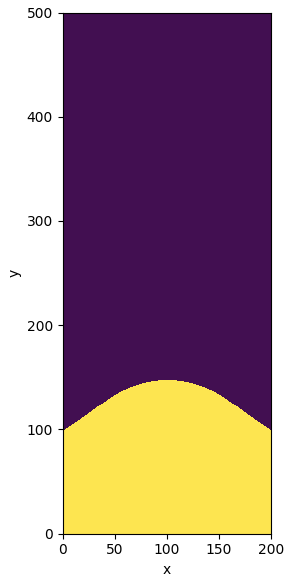
\includegraphics[width=\linewidth]{figures/chap4/rise/series2/580.png}
		\caption{$t=580 \cdot 10^3$}
	\end{subfigure}
	\hfill
	\begin{subfigure}{0.23\textwidth}
		\centering
		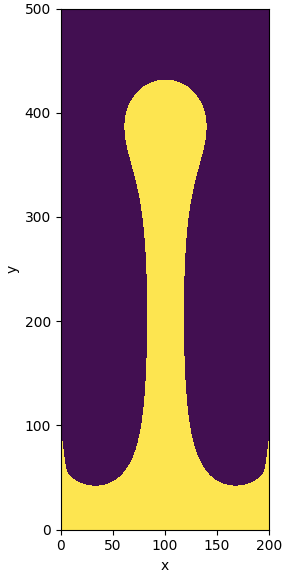
\includegraphics[width=\linewidth]{figures/chap4/rise/series2/625.png}
		\caption{$t=625 \cdot 10^3$}
	\end{subfigure}
	\hfill
	\begin{subfigure}{0.23\textwidth}
		\centering
		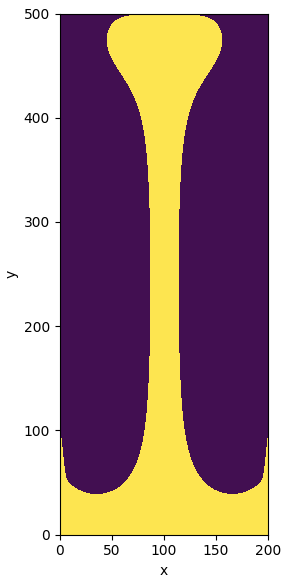
\includegraphics[width=\linewidth]{figures/chap4/rise/series2/635.png}
		\caption{$t=635 \cdot 10^3$}
	\end{subfigure}
	
	\vspace{0.4cm}
	
	% ---- второй ряд ----
	\begin{subfigure}{0.23\textwidth}
		\centering
		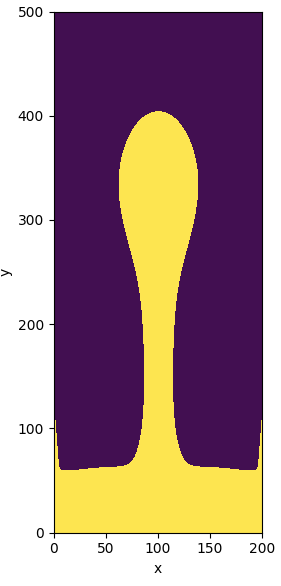
\includegraphics[width=\linewidth]{figures/chap4/rise/series2/660.png}
		\caption{$t=660 \cdot 10^3$}
	\end{subfigure}
	\hfill
	\begin{subfigure}{0.23\textwidth}
		\centering
		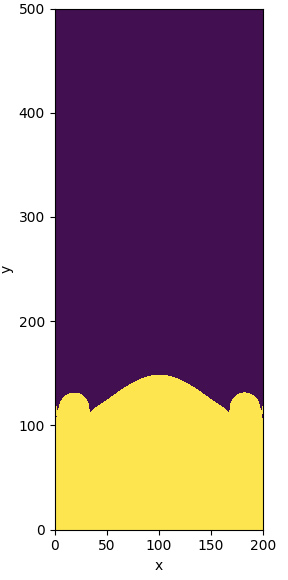
\includegraphics[width=\linewidth]{figures/chap4/rise/series2/670.png}
		\caption{$t=670 \cdot 10^3$}
	\end{subfigure}
	\hfill
	\begin{subfigure}{0.23\textwidth}
		\centering
		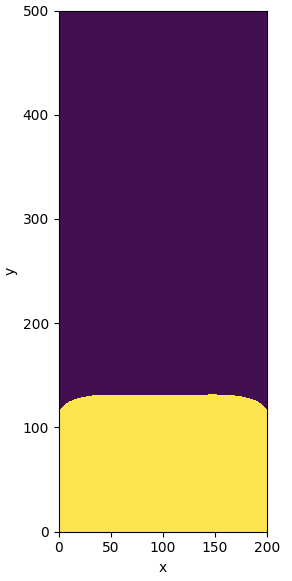
\includegraphics[width=\linewidth]{figures/chap4/rise/series2/700.png}
		\caption{$t=700 \cdot 10^3$}
	\end{subfigure}
	\hfill
	\begin{subfigure}{0.23\textwidth}
		\centering
		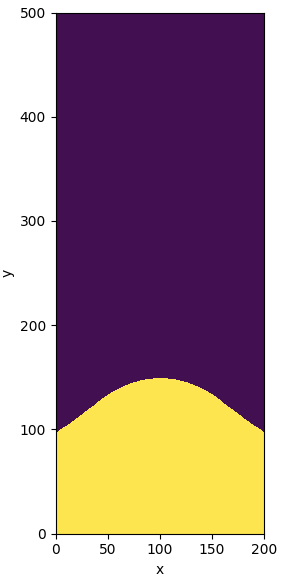
\includegraphics[width=\linewidth]{figures/chap4/rise/series2/780.png}
		\caption{$t=780 \cdot 10^3$}
	\end{subfigure}
	
	\caption{Динамика подъема в различные моменты времени при $\mathrm{Bo}=80$, $\mathrm{We}= 2475$, $\Gamma=2.5$.}
	\label{fig:rise_series_2_LBM}
\end{figure*}

Результаты моделирования показывают, что критическое значение параметра, соответствующее возникновению неустойчивости, то есть моменту, при котором тяжелая жидкость начинает отрываться от дна и терять целостность, находится в интервале $\Gamma \in [0.5, 5]$ и $\mathrm{We} \in [10^2, 10^4]$.

При $\Gamma = 5$ начинается движение тяжелой фазы вверх, однако оно происходит менее эффективно, чем при $\Gamma = 40$. Для промежуточного значения из данного диапазона, а именно при $\Gamma = 2.5$ ($\mathrm{We} = 2475$), наблюдается периодическая структура, однако вибрационного воздействия недостаточно для полного отрыва слоя от дна сосуда (см. рис.~\ref{fig:rise_series_2_LBM}).

При $\Gamma = 0.5$ наблюдаются только колебания межфазной границы без макроскопического перемещения жидкости в целом. Поперечное сечение поля плотности при $x = N_x/2$ для данного случая представлено на рис.~\ref{fig:We_05_LBM}. Оно демонстрирует периодическое движение межфазной границы при сохранении целостности тяжелой фазы.

\begin{figure}
	\centering
	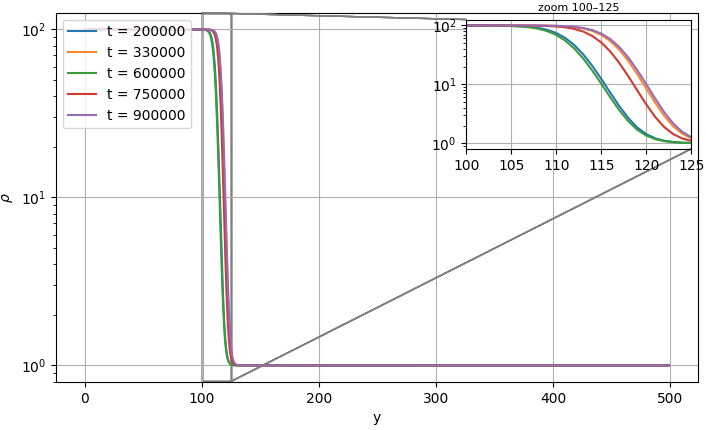
\includegraphics[width=0.85\textwidth]{figures/chap4/rise/We_05}
	\caption{Профиль плотности вдоль оси $y$ при $x=N_x/2$ в различные моменты времени при $\mathrm{Bo} \approx 80$, $\mathrm{We} \approx100$, $\Gamma=0.5$.}
	\label{fig:We_05_LBM}
\end{figure}


%Насколько нам известно, систематическое исследование данной конфигурации ранее не проводилось, хотя сама постановка задачи представляет значительный интерес. В частности, было бы полезно построить карту режимов течения в плоскости параметров $(A,\Omega)$, поскольку проведенные расчеты показывают, что даже при $\Gamma = 40$ различные сочетания амплитуды и частоты могут приводить к качественно различным структурам течения по сравнению с представленными на рис.~\ref{fig:rise_series_LBM}.

%Также представляет интерес исследование влияния отношения плотностей ($\rho_r$) и кинематических вязкостей ($\nu_r$), а также геометрических параметров задачи (размера расчетной области, относительной толщины тяжелого и легкого слоев и т.~д.).

%В настоящей работе мы ограничиваемся демонстрацией возможности моделирования подобных конфигураций и качественной иллюстрацией изменений характера течения, воспроизводимых с помощью разработанного численного алгоритма на основе фазово-полевого метода решеточного Больцмана при вертикальном вибрационном воздействии.

\subsection{Стабилизация тяжелого слоя жидкости в легкой фракции под действием вертикальных вибраций}

В работах \cite{Apffel2020, Apffel2022} была представлена серия изящных экспериментов, в которых вертикальные вибрации использовались для динамической стабилизации границы раздела жидкостей в условиях действия силы тяжести.

Отметим, что в работе \cite{Apffel2020} представлены эксперименты для сосудов различной продольной длины, а также теоретическая модель, связывающая вибрационную и критическую скорости (рассматриваемые ниже). Вместе с тем более ранние эксперименты по подобной стабилизации в небольшом жестком сосуде были представлены в работах \cite{Bezdenezhnykh1982, Bezdenezhnykh1983}, а также в \cite{Wolf1969, Wolf1970}.

В работе \cite{Apffel2020} в одном из экспериментов рассматривался первоначально неподвижный сосуд длиной $L$, заполненный двухслойной системой, состоящей из воздуха и силиконового масла. Затем сосуд подвергался вертикальным гармоническим колебаниям с частотой $f_v = \Omega/2\pi.$
После начала вибраций в нижнюю часть сосуда вводился воздух, в результате чего более тяжелая жидкость оказывалась заключенной между слоями воздуха. Эксперимент показал, что приложенное вибрационное воздействие способствует стабилизации слоя тяжелой жидкости в данной конфигурации.

В работе \cite{Apffel2020} сравниваются две характерные скорости: вибрационная скорость $v_{\mathrm{vibr}} = \mathrm{B} \Omega$ и критическая скорость $v_* = \sqrt{gL/\pi}.$
Показано, что при выполнении условия:
$$
v_{\mathrm{vibr}} > v_*
$$
слой жидкости может устойчиво <<левитировать>> под действием вибраций.

Физические параметры проведенных нами численных экспериментов были выбраны максимально близкими к экспериментальным значениям:
$$
\rho_r=1000, \qquad \nu_r=10, \qquad \mathrm{Bo} \approx 600.
$$
При этом рассматривались различные значения числа Вебера:
$$
\mathrm{We}=0, \qquad \mathrm{We} \approx 3.2 \cdot 10^4, \qquad \mathrm{We} \approx 6 \cdot 10^7.
$$

Для максимально близкого воспроизведения условий эксперимента в качестве начальной конфигурации использовалась трехслойная система, в которой тяжелый слой располагался в области от $y = N_y/4$ до $y = N_y/4 + N_y/5$ (см. рис.~\ref{fig:initial_nature}). Размер расчетной сетки составлял $200 \times 1000$. Такая конфигурация соответствует состоянию системы после введения воздуха, описанному в работе \cite{Apffel2020}.

Начальные скорости во всей расчетной области принимались равными нулю, а вибрационное воздействие прикладывалось начиная с первого шага по времени.

Следует отметить, что важной и перспективной задачей является разработка нового типа граничных условий, предназначенных для точного воспроизведения описанного выше экспериментального режима. Основная идея заключается в формулировке граничных условий для функции распределения параметра порядка таким образом, чтобы коэффициент поверхностного натяжения явно входил в их определение и мог принимать различные значения для легкой и тяжелой фаз. 

В данном исследовании для поля скорости задавались граничные условия свободного скольжения, а для параметра порядка --- условия отсутствия потока. Отметим, что такая постановка не обеспечивает точного воспроизведения рассматриваемого физического эксперимента.

\begin{figure*}
	\centering
	\begin{subfigure}{0.3\textwidth}
		\centering
		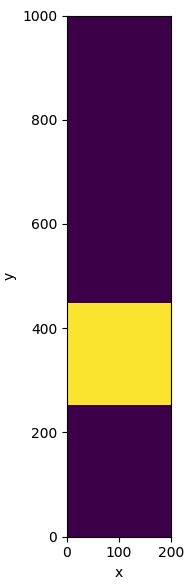
\includegraphics[width=\linewidth]{figures/chap4/nature/initial.png}
		\caption{Начальное распределение}
		\label{fig:initial_nature}
	\end{subfigure}
	\hfill
	\begin{subfigure}{0.3\textwidth}
		\centering
		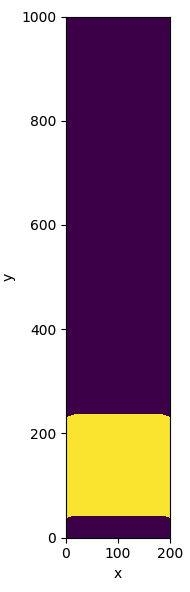
\includegraphics[width=\linewidth]{figures/chap4/nature/We_0/9k.png}
		\caption{$t=9 \cdot 10^3$}
		\label{fig:no_vibro_9k}
	\end{subfigure}
	\hfill
	\begin{subfigure}{0.3\textwidth}
		\centering
		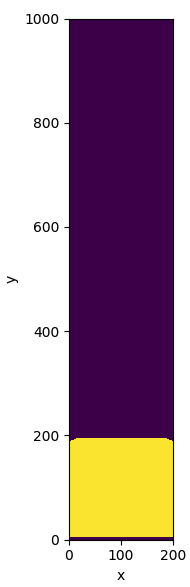
\includegraphics[width=\linewidth]{figures/chap4/nature/We_0/10k.png}
		\caption{$t=10^4$}
		\label{fig:no_vibro_10k}
	\end{subfigure}
	
	\caption{Эволюция процесса опускания тяжелой жидкости в различные моменты времени при $\mathrm{We}=0$, $\mathrm{Bo}\approx 600$.}
	\label{fig:no_vibro_combined_LBM}

\end{figure*}

\begin{figure}
	\centering
	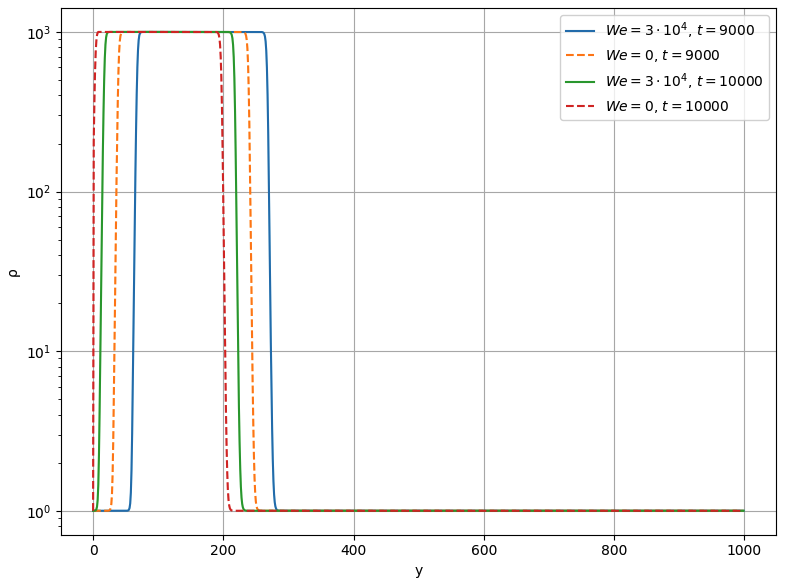
\includegraphics[width=0.75\textwidth]{figures/chap4/nature/log}
	\caption{Профиль плотности вдоль оси $y$ при $x = N_x/2$ для случаев $\mathrm{We} = 0$ и $\mathrm{We} \approx 3.2 \cdot 10^4$, при этом ось $y$ представлена в логарифмическом масштабе, $\mathrm{Bo} \approx 600$.}
	\label{fig:log_density_different_We_LBM}
\end{figure}

В отсутствие вибрационного воздействия ($\mathrm{We} = 0$), как и следовало ожидать, более тяжелая жидкость опускается на дно сосуда (см. рис.~\ref{fig:no_vibro_combined_LBM}). Критическая характерная скорость составляет $v_* = 4.3 \cdot 10^{-2}$. Поэтому при $\mathrm{B} = 100$ и $\Omega = 4 \cdot 10^{-4}$  соответствующее число Вебера остается малым, и динамическая стабилизация не достигается. В этом режиме более тяжелая жидкость продолжает опускаться на дно сосуда, качественно воспроизводя поведение, представленное на рис.~\ref{fig:no_vibro_combined_LBM}.

Тем не менее наличие вибрационного воздействия влияет на динамику системы. На рис.~\ref{fig:log_density_different_We_LBM} показан профиль плотности вдоль оси $y$ при $x = N_x/2$ для случаев $\mathrm{We} = 0$ и $\mathrm{We} \approx 3.2 \cdot 10^4$ в характерные моменты времени $t = 9 \cdot 10^3$ и $t = 10^4$. Полученные результаты показывают, что вибрационное воздействие уменьшает скорость опускания более тяжелой жидкости.

В следующем численном эксперименте амплитуда и частота вибраций были увеличены до $\mathrm{B}= 250$ и $\Omega = 8 \cdot 10^{-4}$ соответственно. Для обеспечения численной устойчивости, при увеличении амплитуды вибраций, характерная скорость была уменьшена до $v_* \approx 5 \cdot 10^{-3}$. Поскольку число Бонда оставалось неизменным, такое изменение не влияло на постановку задачи. При этом усиление вибрационного воздействия сопровождалось ростом числа Вебера от $\mathrm{We} \approx 3.2 \cdot 10^4$ до $\mathrm{We} \approx 6 \cdot 10^7$.

При $\Omega = 8 \cdot 10^{-4}$ период колебаний составляет приблизительно $8000$ безразмерных шагов. Расчет проводился на протяжении примерно 20 вибрационных периодов. На рис.~\ref{fig:We_huge_LBM} представлено поле плотности в течение одного периода в установившемся колебательном режиме. На рис.~\ref{fig:log2_LBM} показан профиль поля плотности вдоль оси $y$ при $x = N_x/2$, причем ось $y$ представлена в логарифмическом масштабе.

\begin{figure*}
	\centering
	\begin{subfigure}{0.23\textwidth}
		\centering
		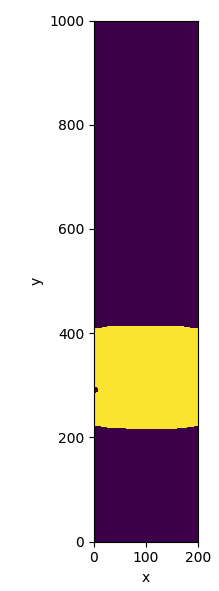
\includegraphics[width=\linewidth]{figures/chap4/nature/We_huge/82.png}
		\caption{$t=82 \cdot 10^3$}
		\label{fig:We_82}
	\end{subfigure}
	\hfill
	\begin{subfigure}{0.21\textwidth}
		\centering
		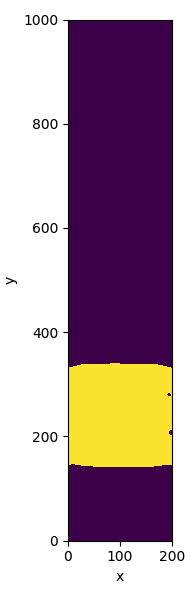
\includegraphics[width=\linewidth]{figures/chap4/nature/We_huge/85.png}
		\caption{$t=85 \cdot 10^3$}
		\label{fig:We_85}
	\end{subfigure}
	\hfill
	\begin{subfigure}{0.215\textwidth}
		\centering
		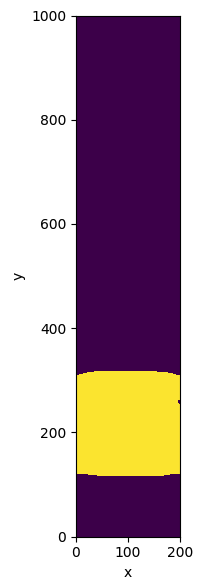
\includegraphics[width=\linewidth]{figures/chap4/nature/We_huge/87.png}
		\caption{$t=87 \cdot 10^3$}
		\label{fig:We_87}
	\end{subfigure}
	\hfill
	\begin{subfigure}{0.23\textwidth}
		\centering
		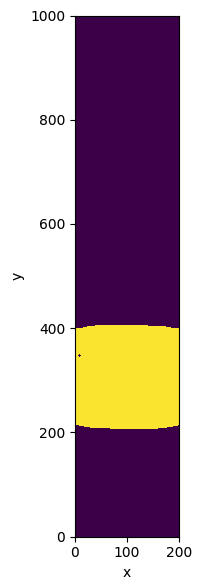
\includegraphics[width=\linewidth]{figures/chap4/nature/We_huge/90.png}
		\caption{$t=90 \cdot 10^3$}
		\label{fig:We_90}
	\end{subfigure}
	
	\caption{Левитация тяжелой жидкости в легкой фазе в течение одного периода вибрационного воздействия при $\mathrm{We} \approx 6 \cdot 10^7$, $\mathrm{Bo} \approx 600$.}
	\label{fig:We_huge_LBM}
\end{figure*}

\begin{figure}
	\centering
	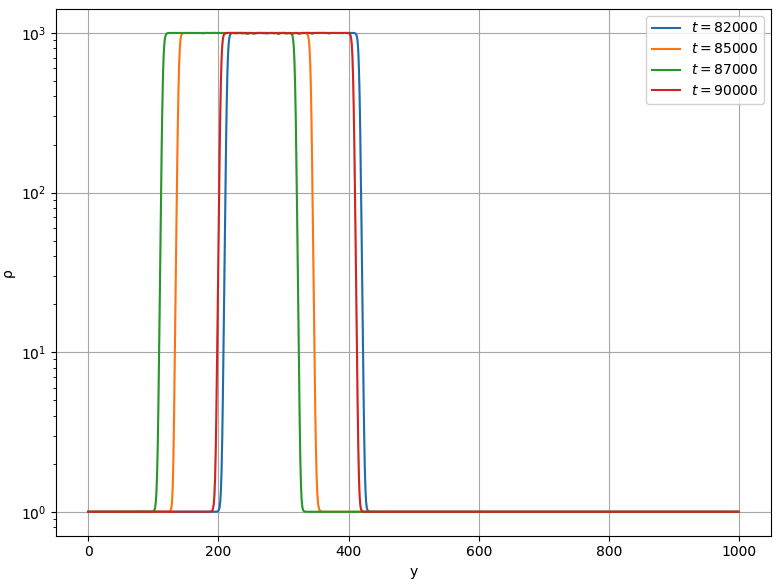
\includegraphics[width=0.75\textwidth]{figures/chap4/nature/We_huge/log}
	\caption{Профиль плотности вдоль оси $y$ при $x = N_x/2$ в различные моменты времени, при этом ось $y$ представлена в логарифмическом масштабе, при $\mathrm{We} \approx 6 \cdot 10^7$, $\mathrm{Bo} \approx 600$.}
	\label{fig:log2_LBM}
\end{figure}

Наконец, был проведен численный эксперимент с двумя слоями тяжелой жидкости при тех же параметрах ($\mathrm{We} \approx 6 \cdot 10^7$, $\mathrm{Bo} \approx 600$) на расчетной сетке $200 \times 2000$. Начальная конфигурация была выбрана таким образом, чтобы два слоя тяжелой жидкости находились на значительном расстоянии друг от друга: первый слой располагался в области от $y = N_y/4$ до $y = N_y/4 + N_y/5$, а второй --- от $y = N_y/4 + 1000$ до $y = N_y/4 + N_y/5 + 1000$.

В работе \cite{Apffel2020} отмечалось, что при выполнении условия
$$
\mathrm{B} \Omega > v_*
$$
несколько слоев тяжелой жидкости могут левитировать под действием вибраций. Данное поведение подтверждается результатами моделирования, представленными на рис.~\ref{fig:two_layers_LBM}, где показано поле плотности в течение одного периода колебаний.

\begin{figure*}
	\centering
	\begin{subfigure}{0.23\textwidth}
		\centering
		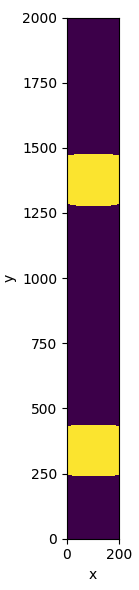
\includegraphics[width=\linewidth]{figures/chap4/nature/two_layers/82.png}
		\caption{$t=82 \cdot 10^3$}
	\end{subfigure}
	\hfill
	\begin{subfigure}{0.225\textwidth}
		\centering
		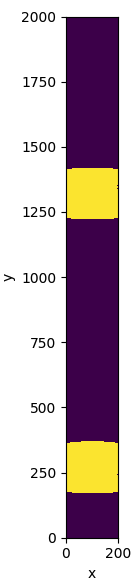
\includegraphics[width=\linewidth]{figures/chap4/nature/two_layers/85.png}
		\caption{$t=85 \cdot 10^3$}
	\end{subfigure}
	\hfill
	\begin{subfigure}{0.23\textwidth}
		\centering
		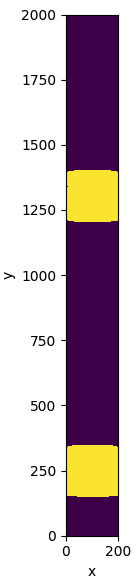
\includegraphics[width=\linewidth]{figures/chap4/nature/two_layers/87.png}
		\caption{$t=87 \cdot 10^3$}
	\end{subfigure}
	\hfill
	\begin{subfigure}{0.23\textwidth}
		\centering
		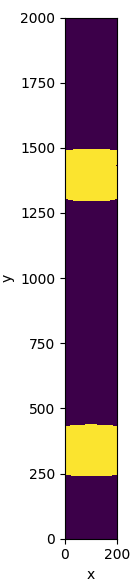
\includegraphics[width=\linewidth]{figures/chap4/nature/two_layers/90.png}
		\caption{$t=90 \cdot 10^3$}
	\end{subfigure}

	\caption{Левитация двухслойной системы в легкой фазе в течение одного периода вибрационного воздействия при $\mathrm{We} \approx 6 \cdot 10^7$, $\mathrm{Bo} \approx 600$.}
	\label{fig:two_layers_LBM}
\end{figure*}

\subsection{Выводы по главе}

В данной главе фазово-полевой метод решеточных уравнений Больцмана был применен для решения задач с протяженной деформируемой свободной границей при вертикальном вибрационном воздействии. Расчеты проведены в широком диапазоне отношений плотностей $\rho_r=3$\textdiv$1000$ и кинематических вязкостей $\nu_r=1/3 $ \textdiv$10$.

Рассмотрена неустойчивость Рэлея--Тейлора. При $\mathrm{Bo}=10$ развитие неустойчивости не наблюдается, поскольку соответствующая неустойчивая мода не укладывается в расчетную область. При $\mathrm{Bo}=200$ неустойчивость развивается, причем основной моде соответствует волновое число $k=2\pi/N_x$. Введение вертикального вибрационного воздействия при $\mathrm{We}=90$ приводит к подавлению основной моды неустойчивости и уменьшению критической длины волны возмущения в два раза.

Представлены результаты численного моделирования гравитационно-капиллярных волн, возбуждаемых вертикальными вибрациями, при $\mathrm{Bo}=160$ и $\mathrm{We}\approx14$ и $\mathrm{We}\approx57$. При меньшем числе Вебера формируются волны слабой интенсивности с небольшой амплитудой. При увеличении числа Вебера в четыре раза при неизменной частоте вибраций амплитуда гравитационно-капиллярных волн существенно возрастает. Аналитическая оценка, основанная на дисперсионном соотношении, показывает хорошее количественное согласие с пространственным периодом формирующейся волновой структуры.

Кроме того, исследована динамика двухфазной системы, состоящей из несмешивающихся жидкостей, находящихся в твердом сосуде при вертикальных вибрациях. Численные расчеты показывают, что достаточно интенсивные вибрации способны вызвать подъем первоначально более тяжелой жидкой фазы к верхней стенке контейнера, несмотря на действие силы тяжести. Наблюдаемое движение имеет нестационарный периодический характер: тяжелая жидкость поднимается, достигает верхней границы, затем частично стекает вниз и вновь поднимается. Показано, что при фиксированных значениях $\rho_r=100$, $\nu_r=1/3$ и $\mathrm{Bo}\approx80$ динамика системы в значительной степени определяется числом Вебера и параметром $\Gamma$. При больших значениях $\Gamma$ реализуется режим макроскопического перемещения тяжелой фазы, сопровождающийся значительной деформацией границы раздела и нарушением ее целостности.

Установлено существование критических параметров вибрационного воздействия, определяющих переход к вибрационно-индуцированному перераспределению жидких фаз. В частности, определен диапазон значений $\Gamma$, соответствующий переходу от режима преимущественно межфазных колебаний к режиму глобального движения жидкости. В интервале $\Gamma\approx0.5$--$5$ система теряет устойчивость: при $\Gamma\approx0.5$ наблюдаются преимущественно колебания межфазной границы без заметного подъема тяжелой фазы, тогда как при $\Gamma\approx5$ возникает подъем тяжелой жидкости. При этом интенсивность ее движения остается существенно ниже, чем в режиме сильного вибрационного воздействия.

Дополнительно выполнено численное исследование конфигурации, близкой к экспериментальным постановкам, посвященным вибрационной стабилизации жидких слоев и связанным с ней эффектам плавучести. Рассмотрена трехслойная система, параметры которой выбраны максимально близкими к физически реалистичным значениям: $\rho_r=1000$, $\nu_r=10$, при фиксированном $\mathrm{Bo}=600$ и различных значениях числа Вебера. В отсутствие вибрационного воздействия тяжелая жидкость оседает на дно контейнера, что соответствует ожидаемому гравитационному поведению системы. Однако даже слабые вибрации изменяют динамику процесса, приводя к уменьшению скорости оседания тяжелой фазы, что проявляется в изменении временной эволюции профилей плотности. С увеличением амплитуды вибраций и, соответственно, числа Вебера система переходит в режим устойчивых колебаний, при котором тяжелая фаза совершает стабильное периодическое движение. Полученные результаты качественно согласуются с экспериментальными наблюдениями, демонстрирующими возможность динамической стабилизации жидких слоев при соответствующем выборе параметров вибрационного воздействия.

Кроме того, промоделирована конфигурация с двумя тяжелыми слоями, разделенными значительным расстоянием. Полученные численные результаты подтверждают экспериментальные выводы о принципиальной возможности стабилизации многослойных структур с помощью вертикальных вибраций.

Дальнейшее совершенствование рассматриваемого численного алгоритма может быть связано с модификацией граничных условий для функции распределения параметра порядка. В частности, перспективным направлением является формулировка граничных условий, в которых коэффициент поверхностного натяжения входит в явном виде и может принимать различные значения для легкой и тяжелой фаз.

Дальнейшие исследования могут развиваться в нескольких направлениях.
Одним из наиболее перспективных представляется моделирование неустойчивости Фарадея, а также переход от двумерной постановки задачи к трехмерной. Отдельного внимания заслуживает применение операторов столкновений типа TRT или MRT. Их использование позволит уменьшить численную диссипацию и снизить величину паразитных течений вблизи межфазной границы при увеличении отношения плотностей и вязкостей фаз. Еще одним перспективным направлением развития метода является его обобщение на неизотермические задачи, что расширит область применимости подхода к моделированию многофазных течений с вертикальным вибрационным воздействием с учетом теплопереноса.


\newpage

\begin{center}
	\section*{Заключение}  
	\addcontentsline{toc}{section}{Заключение}  
\end{center}

Данная диссертация посвящена исследованию влияния вертикальных высокочастотных вибраций на устойчивость и нелинейную динамику межфазных границ в различных физических постановках -- от тонких пленок, описываемых в длинноволновом приближении, до произвольно деформируемых границ раздела несмешивающихся жидкостей, требующих прямого численного моделирования. Такое построение работы позволило исследовать воздействие вибраций с использованием различных подходов к рассмотрению систем: аналитического, применяемого в главах \ref{chap:thermo} и \ref{chap:ferro} и прямого численного, использованного в главе \ref{chap:LBM}. Это дало возможность выявить общие закономерности, характерные для изучаемых систем. 

В главах \ref{chap:thermo} и \ref{chap:ferro} задачи рассматривались в рамках длинноволнового приближения. Для анализа влияния вибрационного воздействия использовалось разложение переменных на быстрые пульсационные и медленно изменяющиеся осредненные компоненты с последующим разделением исходной системы уравнений на соответствующие пульсационную и осредненную части.

В главе \ref{chap:thermo} получены осредненные динамические уравнения жесткого типа для межфазной границы и температуры на границе. Исследована устойчивость границы раздела в линейной постановке, а также проведено численное моделирование нелинейных уравнений. Показано, что вертикальные вибрации способны подавлять неустойчивость тонкой пленки, подогреваемой снизу, конкурируя с дестабилизирующим действием вертикального градиента температуры и связанного с ним термокапиллярного эффекта. Построены карты устойчивости течений при разном значении градиента температуры и для разных гравитационных условий. Проведен слабонелинейный анализ, уточнена граница устойчивости вблизи порога развития неустойчивости.

В главе \ref{chap:ferro} аналогичный подход, основанный на разделении течения на пульсационную и осредненную составляющие в длинноволновом приближении, был использован для анализа динамики межфазной границы магнитной жидкости в стационарном вертикальном магнитном поле в изотермической постановке. Проведен анализ устойчивости течения в линейной постановке. Установлено, что вибрации подавляют как коротковолновую, так и длинноволновую неустойчивость, действуя в этом отношении однонаправленно с поверхностным натяжением.

Таким образом, главы \ref{chap:thermo} и \ref{chap:ferro} демонстрируют, что вибрационная стабилизация межфазной границы является достаточно универсальным эффектом, воспроизводимым при различных дестабилизирующих факторах -- термокапиллярном и магнитном.

В главе \ref{chap:LBM} с помощью фазово-полевого метода решеточных уравнений Больцмана исследована нелинейная динамика систем с деформациями и разрывами межфазной границы. Численно были смоделированы задачи с большим соотношением плотностей и кинематических вязкостей двух несмешивающихся жидкостей. Полученные результаты подтверждают, что вертикальные вибрации способны подавлять развивающиеся неустойчивости и способны стабилизировать конфигурации вплоть до полного изменения топологии равновесия (подъема тяжелой фазы к верхней границе, стабилизации многослойных структур). 

В совокупности полученные результаты формируют целостную картину действия вертикальных вибраций на устойчивость межфазных границ. Как при аналитическом линейном или осредненном описании динамики тонких пленок, так и при прямом численном моделировании показано, что вибрационное воздействие может служить эффективным инструментом управления устойчивостью и структурой многофазных систем для рассмотренных дестабилизирующих механизмов. Это может представлять интерес как для развития теории вибрационной гидромеханики, так и для приложений, связанных с управлением процессами тепло- и массопереноса в тонких пленках и многофазных средах (в том числе в условиях микрогравитации).



\newpage

\addcontentsline{toc}{section}{Список литературы} % Добавляет Список литературы в Содержание
\bibliographystyle{gost2008-1}
\bibliography{thesis_thin_films}

\end{document} 